\documentclass[12pt, letterpaper, twoside]{report}

%%%%%%%%%% RAINBOWFISH packages and commands %%%%%%%%%%%%%%%
\usepackage{microtype}%if unwanted, comment out or use option "draft"

%\graphicspath{{./graphics/}}%helpful if your graphic files are in another directory

\bibliographystyle{plainurl}% the recommended bibstyle

\usepackage{graphicx}
\usepackage{pgfplots}
\usepackage{pgfplotstable}

\usepgfplotslibrary{external}
\tikzexternalize[prefix=figs/]

\usepgfplotslibrary{groupplots}
\pgfplotsset{compat=newest}
\usepackage{caption}
\usepackage[skip=-3pt,belowskip=4pt]{subcaption}

\usepackage{xspace} % deals with the problem of when you want spaces
                    % after a macro
\usepackage{textcomp}
\usepackage{balance}  % for  \balance command ON LAST PAGE  (only there!)
\usepackage{xcolor}
\usepackage{amsmath}
\usepackage{algorithm}
\usepackage{algorithmicx}
\usepackage{cite}
\usepackage{float}
\usepackage{tablefootnote}
\usepackage{enumitem} % package for easily changing list parameters
\usepackage[noend]{algpseudocode}
%\usepackage{natbib}
\usepackage{url}
\usepackage{hyperref}
% \usepackage{fullpage}
%\usepackage[margin=1in]{geometry} % I think that geometry now improves
                                % upon fullpage. 

%\usepackage{our-comments}

\usepackage{siunitx}
\usepackage{amssymb}
\usepackage{color}
\usepackage{booktabs}
\usepackage[capitalise,nameinlink]{cleveref}

\usepackage{wrapfig}
\usepackage{times}

\usepackage{amsthm}
%TODO very important!! WTH is this
%\DeclareUnicodeCharacter{00A0}{ }

\usepackage{tabularx}
%\newcolumntype{L}{>{\raggedright\arraybackslash}X}

\usepackage[compact]{titlesec}
\titlespacing{\section}{0pt}{2ex}{1ex}
\titlespacing{\subsection}{0pt}{1ex}{0ex}
\titlespacing{\subsubsection}{0pt}{0.5ex}{0ex}


\newcommand{\defn}[1]{{\textit{\textbf{\boldmath #1}}}}
\newcommand{\cqf}{counting quotient filter\xspace}
\newcommand{\cqfs}{counting quotient filters\xspace}
\newcommand{\dbg}{de Bruijn graph\xspace}
\newcommand{\dbgs}{de Bruijn graphs\xspace}
\newcommand{\wdbg}{weighted de Bruijn graph\xspace}
\newcommand{\wdbgs}{weighted de Bruijn graphs\xspace}
\newcommand{\Wdbg}{Weighted de Bruijn Graph\xspace}
\newcommand{\Wdbgs}{Weighted de Bruijn Graphs\xspace}
\newcommand{\cdbg}{colored de Bruijn graph\xspace}
\newcommand{\cdbgs}{colored de Bruijn graphs\xspace}
\newcommand{\Cdbg}{Colored de Bruijn Graph\xspace}
\newcommand{\Cdbgs}{Colored de Bruijn Graphs\xspace}
\newcommand{\compdbg}{compacted de Bruijn graph\xspace}
\newcommand{\dBG}{de Bruijn graph\xspace}
\newcommand{\dBGs}{de Bruijn graphs\xspace}
\newcommand{\cf}{cuckoo filter\xspace}
\newcommand{\bloomf}{Bloom filter\xspace}
\newcommand{\cbf}{counting Bloom filter\xspace}
\newcommand{\vect}[1]{\left[#1\right]}
\newcommand{\set}[1]{\left\{#1\right\}}
\newcommand{\seq}[1]{\left(#1\right)}
\renewcommand{\epsilon}{\varepsilon}
\newcommand{\ceil}[1]{\left\lceil #1 \right\rceil}
\newcommand{\kmers}{$k$-mers\xspace}
\newcommand{\kmer}{$k$-mer\xspace}
\newcommand{\kmc}{KMC2\xspace}
\newcommand{\jelly}{Jellyfish2\xspace}
\newcommand{\squeakr}{Squeakr\xspace}
\newcommand{\squeakrs}{Squeakr}
\newcommand{\squeakre}{Squeakr (exact)\xspace}
\newcommand{\rainbowfish}{Rainbowfish\xspace}
\newcommand{\order}[1]{\ensuremath{O(#1)}}
\newcommand{\vari}{VARI\xspace}
\newcommand{\boss}{BOSS\xspace}
\newcommand{\ecoli}{\emph{E. coli}\xspace}
\newcommand{\plant}{Plant\xspace}
\newcommand{\beefsafety}{Beef safety\xspace}
\newcommand{\rank}{\mbox{\sc rank}}
\newcommand{\select}{\mbox{\sc select}}
\newcommand{\rrr}{RRR\xspace}
\newcommand{\bracken}{bracken\xspace}
\newcommand{\kraken}{kraken\xspace}
\newcommand{\karp}{karp\xspace}
\newcommand{\minimap}{minimap2\xspace}
\newcommand{\eq}{equivalence class\xspace}
\newcommand{\eqs}{equivalence classes\xspace}
\newcommand{\Reads}{\ensuremath{\mathcal{R}}\xspace}
\newcommand{\abpt}{\textit{PR}\xspace}
\newcommand{\fraglen}[1]{\ensuremath{d_{#1}}}

\newcommand\fnurl[2]{%
  \href{#2}{#1}\footnote{\url{#2}}%
}
\newcommand{\cfun}[1]{\ensuremath{\texttt{Col}(#1)}}
\newcommand\etal{et al.\xspace}
%\newcommand{\fatemeh}[1]{\textcolor{orange}{[#1]}}
\newcommand{\cortex}{\texttt{Cortex}\xspace}
\setlength{\belowcaptionskip}{-0pt}
\newtheorem{lemma}{Lemma}
\newtheorem{theorem}{Theorem}

%%%%%%%%%% RAINBOWFISH packages and commands %%%%%%%%%%%%%%%




%%%%%%%%%% PUFFERFISH packages and commands %%%%%%%%%%%%%%%
\usepackage{cmap}
\usepackage[T1]{fontenc}
%\usepackage[square,sort,comma,numbers]{natbib}
%\usepackage{graphicx}
\usepackage{bm}

%\usepackage{amsmath}
%\usepackage{algorithm}
%\usepackage[noend]{algpseudocode}
\usepackage{multirow}
%\usepackage[justification=centering]{caption}

\makeatletter
\def\BState{\State\hskip-\ALG@thistlm}
\makeatother

%Even though `american`, `english` and `USenglish` are synonyms for babel package (according to https://tex.stackexchange.com/questions/12775/babel-english-american-usenglish), the llncs document class is prepared to avoid the overriding of certain names (such as "Abstract." -> "Abstract" or "Fig." -> "Figure") when using `english`, but not when using the other 2.
%english has to go last to set it as default language
\usepackage[ngerman,english]{babel}
%Hint by http://tex.stackexchange.com/a/321066/9075 -> enable "= as dashes
\addto\extrasenglish{\languageshorthands{ngerman}\useshorthands{"}}

%better font, similar to the default springer font
%cfr-lm is preferred over lmodern. Reasoning at http://tex.stackexchange.com/a/247543/9075
\usepackage[%
rm={oldstyle=false,proportional=true},%
sf={oldstyle=false,proportional=true},%
tt={oldstyle=false,proportional=true,variable=true},%
qt=false%
]{cfr-lm}
%
%if more space is needed, exchange cfr-lm by mathptmx
%\usepackage{mathptmx}

%for demonstration purposes only
\usepackage[math]{blindtext}

%Sorts the citations in the brackets
%It also allows \cite{refa, refb}. Otherwise, the document does not compile.
%  Error message: "White space in argument"
%\usepackage{cite}


%% If you need packages for other papers,
%% START COPYING HERE
%% COPY ALSO cmap and fontenc from lines 10 to 12

%extended enumerate, such as \begin{compactenum}
% \usepackage{paralist}

%put figures inside a text
%\usepackage{picins}
%use
%\piccaptioninside
%\piccaption{...}
%\parpic[r]{\includegraphics ...}
%Text...

%for easy quotations: \enquote{text}
\usepackage{csquotes}

%enable margin kerning
%\usepackage{microtype}

%tweak \url{...}
%\usepackage{url}
%\urlstyle{same}
%improve wrapping of URLs - hint by http://tex.stackexchange.com/a/10419/9075
\makeatletter
\g@addto@macro{\UrlBreaks}{\UrlOrds}
\makeatother
%nicer // - solution by http://tex.stackexchange.com/a/98470/9075
%DO NOT ACTIVATE -> prevents line breaks
%\makeatletter
%\def\Url@twoslashes{\mathchar`\/\@ifnextchar/{\kern-.2em}{}}
%\g@addto@macro\UrlSpecials{\do\/{\Url@twoslashes}}
%\makeatother

%diagonal lines in a table - http://tex.stackexchange.com/questions/17745/diagonal-lines-in-table-cell
%slashbox is not available in texlive (due to licensing) and also gives bad results. This, we use diagbox
%\usepackage{diagbox}

%required for pdfcomment later
%\usepackage{xcolor}


%enable nice comments
%this also loads hyperref
\usepackage{pdfcomment}
%enable hyperref without colors and without bookmarks
\hypersetup{hidelinks,
   colorlinks=true,
   allcolors=black,
   pdfstartview=Fit,
   breaklinks=true}
%enables correct jumping to figures when referencing
\usepackage[all]{hypcap}

\newcommand{\commentontext}[2]{\colorbox{yellow!60}{#1}\pdfcomment[color={0.234 0.867 0.211},hoffset=-6pt,voffset=10pt,opacity=0.5]{#2}}
\newcommand{\commentatside}[1]{\pdfcomment[color={0.045 0.278 0.643},icon=Note]{#1}}

%compatibality with packages todo, easy-todo, todonotes
\newcommand{\todo}[1]{\commentatside{#1}}
%compatiblity with package fixmetodonotes
%\newcommand{\TODO}[1]{\commentatside{#1}}

%enable \cref{...} and \Cref{...} instead of \ref: Type of reference included in the link
%\usepackage[capitalise,nameinlink]{cleveref}
%Nice formats for \cref
\crefname{section}{Sect.}{Sect.}
\Crefname{section}{Section}{Sections}

\newtheorem{thm}{Theorem}
\newtheorem{observation}[thm]{\textbf{Observation}}
%\newcommand{\eg}{e.\,g.\xspace}
%\newcommand{\ie}{i.\,e.\xspace}
\newcommand{\eg}{e.\,g.,\ }
\newcommand{\ie}{i.\,e.,\ }
%\newtheorem{observation}[thm]{\textbf{Observation}}
\newcommand{\pufferfish}{pufferfish\xspace}
\newcommand{\bv}{\texttt{bv}\xspace}
\newcommand{\ctab}{\texttt{ctab}\xspace}
\newcommand{\cseq}{\texttt{cseq}\xspace}
\newcommand{\kallisto}{Kallisto\xspace}
\newcommand{\bwa}{BWA\xspace}
\newcommand{\twopaco}{TwoPaCo\xspace}
\newcommand{\ccdbg}{compacted de Bruijn graph\xspace}
\newcommand{\ccdbgs}{compacted de Bruijn graphs\xspace}

%introduce \powerset - hint by http://matheplanet.com/matheplanet/nuke/html/viewtopic.php?topic=136492&post_id=997377
\DeclareFontFamily{U}{MnSymbolC}{}
\DeclareSymbolFont{MnSyC}{U}{MnSymbolC}{m}{n}
\DeclareFontShape{U}{MnSymbolC}{m}{n}{
    <-6>  MnSymbolC5
   <6-7>  MnSymbolC6
   <7-8>  MnSymbolC7
   <8-9>  MnSymbolC8
   <9-10> MnSymbolC9
  <10-12> MnSymbolC10
  <12->   MnSymbolC12%
}{}
\DeclareMathSymbol{\powerset}{\mathord}{MnSyC}{180}

% correct bad hyphenation here
\hyphenation{op-tical net-works semi-conduc-tor}

%% END COPYING HERE

%%%%%%%%%% PUFFERFISH packages and commands %%%%%%%%%%%%%%%



\usepackage[margin=1in]{geometry}
\usepackage[utf8]{inputenc}
\usepackage{etex}
%\usepackage{amsmath}
%\usepackage{graphicx}
%\usepackage{hyperref}
%\usepackage{url}
%\usepackage{todonotes}
%\usepackage{bm}
%\usepackage{xspace}
%\usepackage{booktabs}
\usepackage{adjustbox}
%\usepackage[font=footnotesize]{subcaption}
%\usepackage[font=footnotesize]{caption}
\captionsetup{belowskip=4pt,aboveskip=4pt}
%\usepackage{float}

\usepackage{etoolbox}

%%%%%%%%%% MANTIS packages and commands %%%%%%%%%%%%%%%
%\usepackage{pgfplots}
%\usepackage{pgfplotstable}
\usepgfplotslibrary{groupplots}
\pgfplotsset{compat=newest}
%\usepackage{textcomp}
%\usepackage{xcolor}
%\usepackage{amsmath}
\usepackage{mathtools}
%\usepackage{algorithm}
%\usepackage{algorithmicx}
%\usepackage{cite}
%\usepackage{float}
%\usepackage{tablefootnote}
%\usepackage{enumitem}
%\usepackage[noend]{algpseudocode}
%\usepackage{url}
%\usepackage{hyperref}
%\usepackage[margin=1in]{geometry}
%\usepackage{siunitx}
%\usepackage{amssymb}
%\usepackage{color}
%\usepackage{booktabs}
%\usepackage{wrapfig}
%\usepackage{multirow}

\usepackage[numbers]{natbib}
%\usepackage{bibalias}
%\usepackage{cleveref}
\usepackage{pbox}
\usepackage{fancyhdr}


% HERE'S HOW WE SWITCH COMMENTS ON AND OFF
\newif\ifcomments        % here's how we switch comments on and off
\commentstrue
%\commentsfalse

\usepackage{our-comments} % here's where we define how we write

\theoremstyle{definition}
\newtheorem{definition}{Definition}[section]

\DeclareRobustCommand{\bigO}{%
\text{\usefont{OMS}{cmsy}{m}{n}O}%
}

\newcommand\ourparagraph[1]{\paragraph*{\bf{#1}}}

\renewcommand{\defn}[1]       {{\textit{#1}}}


\newcommand{\contains}{\textsc{contains}\xspace}
\newcommand{\mantis}{Mantis\xspace}
\newcommand{\sbt}{SBT\xspace}
\newcommand{\sbtallsome}{SBT-AllSome\xspace}
\newcommand{\ssbt}{SSBT\xspace}
\newcommand{\allsomesbt}{AllSomeSBT\xspace}
\newcommand{\longcdbg}{colored de Bruijn graph\xspace}
\newcommand{\longcdbgs}{colored de Bruijn graphs\xspace}
\newcommand{\longCdbgs}{Colored de Bruijn graphs\xspace}
\newcommand{\blf}{Bloom filter\xspace}
\newcommand{\blfs}{Bloom filters\xspace}

\newcommand{\vesca}{\textit{F. vesca}\xspace}
\newcommand{\gallus}{\textit{G. gallus}\xspace}
\newcommand{\balbisiana}{\textit{M. balbisiana}\xspace}
\newcommand{\sapiens}[1]{\textit{H. sapiens #1}\xspace}

\newcommand{\mst}{MST\xspace}
\newcommand{\mstfull}{Minimum Spanning Tree\xspace}
\newcommand{\cbv}{color bit-vector\xspace}
\newcommand{\cbvs}{color bit-vectors\xspace}
\newcommand{\cc}{color class\xspace}
\newcommand{\ccs}{color classes\xspace}
\newcommand{\bbb}{BBB\xspace}
\newcommand{\kruskal}{Kruskal\xspace}
\newcommand{\seqothello}{SeqOthello\xspace}
\newcommand{\tp}{True Positive\xspace}
\newcommand{\tps}{True Positives\xspace}
\newcommand{\fp}{False Positive\xspace}
\newcommand{\fps}{False Positives\xspace}
\newcommand{\fn}{False Negative\xspace}
\newcommand{\fns}{False Negatives\xspace}
\newcommand{\bbv}{boundary bit-vector\xspace}
\newcommand{\dbv}{delta vector\xspace}
\newcommand{\pbv}{parent vector\xspace}
\newcommand{\ccid}{\text{ccID}\xspace}
\newcommand{\idcc}{\text{cc}\xspace}
\newcommand{\colorid}{color-class ID\xspace}
\newcommand{\colorids}{color-class IDs\xspace}
\newcommand\calC{\ensuremath{\mathcal{C}}}
\newcommand\calD{\ensuremath{\mathcal{D}}}
\setlength{\belowcaptionskip}{-5pt}
\captionsetup[subfigure]{skip=7pt}

%%%%%%%%%% MANTIS packages and commands End %%%%%%%%%%%%%%%

\newcommand{\abs}[1]{\left|#1\right|}



\newcommand{\thatis}{i.e.\xspace}
\newcommand{\forexample}{e.g.\xspace}
\newcommand{\andothers}{et al.\xspace}
% Enter dates of publication


\title{Algorithms and Data Structures for Indexing, Querying and Analyzing Large Collections of Sequencing Data in the Presence or Absence of a Reference}

\author{\\ \\ \textbf{Fatemeh Almodaresi} \\ \\ \\ \textbf{Committee Members:} \\ Professors \\ Rob Patro (advisor) \\ Hector Corrada \\ Mihai Pop \\ David Mount \\ \\ \\ \textbf{Department of Computer Science} \\ \textbf{University of Maryland at College Park} \\ \\ \\ Thesis Proposal \\ \\ }

\date{ December 2019}

 
\begin{document}

\begin{titlepage}
\maketitle
\end{titlepage}
 
\begin{abstract}
    \normalsize
RNA sequencing is a popular asset for measuring transcriptomes and
is useful for sequence alignment, expression quantification, and sequence assembly of genes and transcripts.
The vast amount of available raw RNA sequences, and its growth rate over the past decade
brings us with an important
computational challenge prior to any higher level analytical tasks
which is a memory-efficient data structure for indexing the underlying set of sequences
that provides a time-efficient query.

This challenge is not limited to only raw RNA sequences.
By the continuing assembly of novel genomes and transcriptomes,
specifically in metagenomics, having an efficient index over the list of assembled sequences is
still an ongoing challenge. To be specific,
there is still a high demand for an index providing a balance between memory and query time.

We have developed new data structures to substantially reduce the memory used by these indices
and still achieve similar query speed.
These are highly promising data structures for sequence search, sequence alignment, or sequence assembly
and are useful for transcriptomic, genomic, metagenomic, and microbiome analysis.

We can divide these data structures into two categories of reference-based and reference-free indices.
We propose three separate indices,
one over the set of reference sequences used for alignment and mapping applications called Pufferfish,
one over a set of raw sequences designed to be accessed for assembly, variant detection and bubble calling
called Rainbowfish,
and a third one also being over a big set of sequences, but used in sequence search applications called Mantis.
All these data structures are based on de Bruijn graph and different variations of it
such as colored de Bruijn graph or compacted de Bruijn graph.

Specifically we designed a new, succinct representation for the color information
of colored de Bruijn graphs in “Rainbowfish”.
This representation can be used in de novo assembly and variant detection
to keep information about the sample of origin of each k-mer when combining many samples.
For example, our data structure allows build a colored de Bruijn graph
on a metagenomic data set in just a few gigabytes
while the space state-of-the-art data structures take is hundreds of gigabytes,
showing an order-of-magnitude improvement.
Moreover, the query time for searching a k-mer and fetching the color information
in our representation is almost the same as the existing data structures.

Using a similar representation as Rainbowfish to store the list of samples each k-mer appears in
, combined with Counting Quotient Filter to find the index associated to each k-mer we've developed Mantis,
a space-frugal index over thousands of samples with a fast query time up to 106 percent faster than
the sequence search tools at the time.
Mantis is also a colored de Bruijn graph representation,
so it supports fast graph traversal and other topological analyses
in addition to large-scale sequence-level searches.

Later, we update the color information representation
by adopting a hierarchical encoding that exploits correlations among color vectors.
We apply this encoding in the context of two different applications;
the implicit cdbg used for a large-scale sequence search index,
Mantis, as well as the encoding of color information used in
population-level variation detection tool, Rainbowfish.
Our results show significant improvements in the overall size and
scalability of representation of the color information.

In Pufferfish, however, we've developed a new data structure for indexing large-scale reference sequences,
or large collections of reference sequences rather than raw sequence samples by building an index
for the compacted, colored de Bruijn graph over the reference sequences.
We have developed both a sparse and dense indexing scheme which allows one
to trade off index space for query speed
(though queries always remain asymptotically optimal).
In addition to indexing the k-mers, we store informations such as
position and orientation of each k-mer in the reference set.
This space-efficient data structure is built on top of
the compacted representation of de Bruijn graph and hence will work well as an index
for purposes such as alignment and quantification.

In designing all the above methods, we make use of techniques
from succinct data structure design — building more complex operations atop bit vectors
and the rank and select operations and also minimum perfect hashing to help substantially reduce the memory
required for compacted de Bruijn graph indexing.

For my thesis, I propose advancing the ideas explained earlier in two specific, but separate direction.
For the reference-base index scheme, I focus on one of the applications of Pufferfish as the alignment tool
used in estimating abundance of known genomes
    in metagenomic analysis. This work is along the tools such as Bracken and Karp and slightly different from
    metagenomic classification methods such as Kraken. In addition to that, I will continue working on
    the scalability limits of Mantis as a large-sequence-search index by investigating the potentials of
    merging two manti without the need to construct the color information in bit vector format and convert it
    to the hierarchical structure and by controlling the construction memory in a limited range
with respect to the size of the input data.


% de Bruijn graphs are nowadays an inseparable part of Next Generation Sequence analyses. With the fast growth in the amount of sequencing reads and variety of different genomes and transcriptomes the community is shifting toward using graphs to represent collections of references and map reads. 
% In this document, we present two succinct representations for two different variations of a de Bruijn graph, namely colored de Bruijn graph and compacted de Bruijn graph. For the former, we designed and developed rainbowfish, a succinct data structure to represent colors for an efficient \dbg representation and also theoretically proved why we call it succinct. This structure is useful in genome variant detection and genotyping. For the later, we developed a tool named pufferfish for indexing a compacted de Bruijn graph in two different schemes of dense and sparse. While being close to linear indexing methodologies regarding memory, pufferfish shows to have a similar \kmer lookup speed as other memory-consuming de Bruijn graph indexing schemes. The balance that pufferfish offers between memory and speed makes it suitable for large-scale indexing such as for collections of RNA-seq data or in metagenomic analysis.
\end{abstract} 

\newpage

\tableofcontents

\newpage

%\usepackage{natbib}

\chapter{Introduction}

\paragraph*{Why was this topic important to investigate?}

Deep next generation sequencing, producing millions of short RNA reads per sample,
has become a great asset for tasks such as transcriptome abundance estimation, and
assembly as well as providing a rich database of information over hundreds of thousands of individuals
with associated meta-data and extensive variation. The low-cost and simple protocol for
producing short reads has provided the community with massive collections of raw sequence samples.
In addition to the large collections of raw sequence samples,
there exist large databases of assembled genomes and transcriptomes
due to computational advancements in sequence assembly
using RNA reads specifically in the domain of metagenomics.
There has been a lot of effort and research in organizing and indexing these databases
and extracting information from them efficiently~\cite{paten2017genome}.
Such indices have been used in various computational
and biological applications such as alignment and mapping,
genome and transcriptome abundance estimation and differential expression,
and genome and transcriptome assembly and variation/isoform detection.
In addition to all these applications, these databases themselves are a great resource
of information to find out sequence-based novelties, differences, disparities and abnormalities
across different species, individuals, tissues, or even single cells.
To extract and analyze this information, the role of a dynamic and efficient search index
over such big databases of (short raw and long assembled) sequences
with the ability of quick queries is essential.
The amount of research done in the past decade on building indices over
the genomic and transcriptomic sequences and the tremendous use of those tools by biologists
in their analyses adds to the importance of this matter and its usefulness.

%\paragraph*{What did we know about this topic before I did this study?}
\paragraph*{}
While there have been a wide variety of tools developed
for indexing and querying large collections of sequences in the past
~\citep{li2008mapping,langmead2009ultrafast,li2009fast,hach2010mrsfast,langmead2012fast,li2013aligning,liao2013subread,dobin2013star,kim2015hisat},
we can divide them into two main categories of linear- and graph-based indices.
In the linear-based approaches, the series of sequences are put together and treated as one large text
and then indexed based on well-known data structures for indexing large-text sequences
such as FM-index or suffix arrays
~\citep{langmead2009ultrafast,li2009fast,langmead2012fast,li2013aligning,dobin2013star,kim2015hisat}.
These indices (also called full-text indices) are usually very small, compared to the size of the
raw data they index but can be slow to query.
On the other hand, the graph-based indices make use of factoring out the repeats in the sequences
to reduce the size of the index and provide faster queries.
In these approaches, a sequence is
splitted into sub-sequences of size k (called a \kmer) where each \kmer is presented only once
in the whole index.
Yet, although much faster than the full-text approaches, they are often orders of magnitude larger.
Therefore, having an index with a balance between the memory and query time
is still a continuing challenge that requires solving computational problems by applying
existing algorithms in other areas of computer science or developing new ones.

One of the mostly used types of graph in graph-based indexing is the \dbg
and its variants, the \longcdbg (cdbg), the \compdbg, and the compacted \longcdbg.
I’ve worked on two particular problems. The first is succinct representation of membership information
in a \longcdbg, and the second is efficient indexing for \kmers
in a compacted \longcdbg.
Below I provide a brief overview of previous works on graph-based representation,
along with common use cases of the various algorithms and methods developed.

\section{De Bruijn Graph}
\label{subsec:dbg}
A \dbg (dbg) is a directed graph representing a set of sequences.
This type of graph has two variants, node-centric and edge-centric.
In the edge-centric \dbg, each directed edge is a unique substring of length $k$ in the sequence set,
which we call a \kmer. Each edge has a prefix overlap of $k-1$ bases with the source node
and a suffix overlap of length $k-1$ with the destination node~\cite{paten2017genome}.
Figure~\ref{fig:dbg-a} shows a simple \dbg for a sample with one string.
This type of graph is designed so that by having a walk through edges and
putting all edges next to each other with overlaps of $k-1$,
we are able to build the reference sequence, such as a gene or transcript,
as shown in~\ref{fig:dbg-b}. Ofcourse it is worth noting that such ``perfect assembly''
is not always possible due to sequencing errors, repeats, and other complexities that come in the way.
In the node-centric variant of a \dbg, each node represents a \kmer,
connected by overlapping strings in the same way.

\begin{figure}
    \centering
    \begin{subfigure}{.5\textwidth}
        \centering
        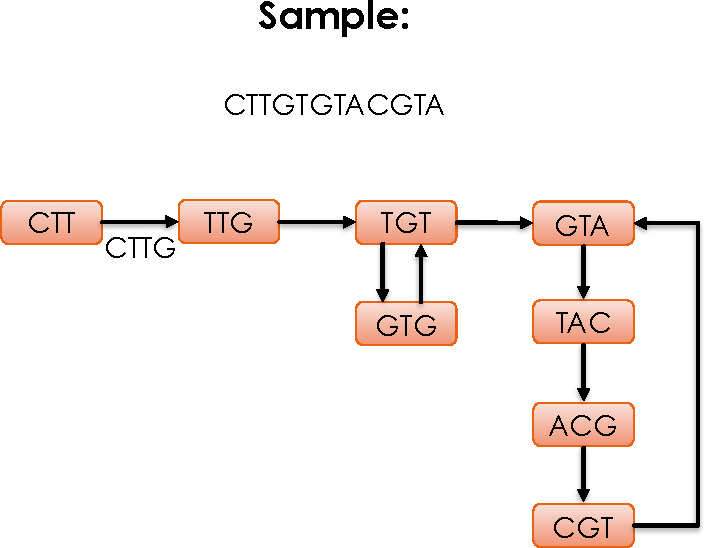
\includegraphics[width=\linewidth]{figs/dbg1-cropped.pdf}
        \caption{de Bruijn graph for a sample with one sequence.}
        \label{fig:dbg-a}
    \end{subfigure}%
    \begin{subfigure}{.5\textwidth}
        \centering
        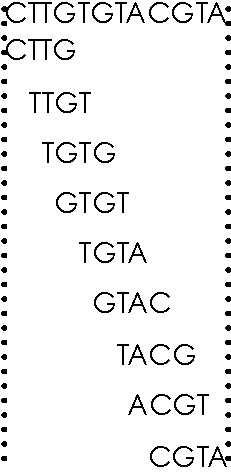
\includegraphics[width=.4\linewidth]{figs/dbg2-cropped.pdf}
        \caption{This example shows how one can reconstruct the reference sequence
        having a walk through nodes and edges in a de Bruijn graph and taking care of overlaps.}
        \label{fig:dbg-b}
    \end{subfigure}
    \caption{Building a de Bruijn graph and reconstructing the reference sequence from it}
    \label{fig:dbg}
\end{figure}

The \dbg is a useful structure for indexing a reference or set of sequencing reads
because it enables fast querys.
One drawback is that for the $k-1$ overlaps between consequent edges,
the original data structure is very space-inefficient. For example,
ABYSS~\cite{simpson2009abyss} represents the \dbg as a hash table with each \kmer
as the key and a byte keeping all the connections to other nodes as its value.
It needs $1$ bit to show the existence of each of the edges in forward or reverse-complement case
(as we have four characters in our alphabet, we can expand the current node
to reach to the next one in at most four different ways in forward direction).
The space such a data structure takes is $\abs{E_s}(\frac{k}{4}+1)\frac{1}{\gamma}$ bits
where $\gamma \leq 1$, is the hash table loading factor.
This storage is considerably large for even one genome data set,
such as the human genome (starting from 40GB while depending on the loading factor can grow to 100GB or more).
Yet, a few different data structures and algorithms have been proposed to reduce the size of a \dbg
and represent it efficiently. One category of these data structures use the Bloom Filter~\cite{}
to represent a \dbg~\cite{pell2012scaling,salikhov2013using,chikhi2012space,chikhi2013space,holley2016bloom}.
Other than these, there are a few proposed representations
that rely on succinct data structures~\cite{gbmp2014sea}
and rank and select operations including the original work by Conway and Bromage~\cite{conway2011succinct}
and later the work in~\cite{BoweOn12} that is called the BOSS representation of \dbg from the authors’ initials.
BOSS is an efficient, edge-centric representation of \dbg that takes around 3 bits per \kmer,
which is considerably smaller than the hash table representation.
This representation provides a mechanism for navigation through the \dbg
and also an interface to interact and get access to the ID of each \kmer.
In section~\ref{chap:rainbowfish}, I explain in more detail, our work on the color representation
for a \dbg built on top of the BOSS structure, using the interface it provides.


\subsection{Compacted \dbg}
\label{subsubsec:cdbg}
The main advantage of a \ccdbg is being more space-efficient compared to the
classic representation of the \dbg due to the nodes representing
paths with no branches rather than \kmers.
The process of compacting the \dbg is meant to merge all \kmers in a non-branching path
in the \dbg with outgoing and incoming degrees of
one into a single node which is called a \emph{unitig}.
The output of this step is called a \compdbg,
that connects these unitigs and is a variant of the original \dbg
with unitigs as nodes rather than the \kmers.
This can be used in the same way as a \dbg for different downstream applications,
such as mapping, alignment, variant detection, etc.
This method reduces memory by eliminating the great amount of overlaps of $k-1$ bases
repeated in consequent \kmers.
For instance, the output node after merging two consequent nodes in a node-centric \dbg
with overlap of $k-1$ would be a unitig of length $k+1$ where the node starts with the first base in the source node,
continues with the $k-1$ overlapping bases and ends in
the last base of the destination.
This compaction step can have a great impact on reducing the memory
and is very useful in cases that we are dealing with repeat-heavy sequences~\cite{liu2016debga}.
Recently, researchers have designed and implemented algorithms for building
a \ccdbg directly from raw data instead of building the memory-inefficient \dbg first
and then compacting it~\cite{minkin2016twopaco,chikhi2016compacting}.
However, indexing a \ccdbg is still a challenge that needs further investigation.

%\paragraph*{How will this study advance new knowledge or new ways of understanding?}
\paragraph*{}
%\fatemeh{Is this still true?}
So far, we know of two other tools, kallisto~\cite{Bray2016Kallisto}
, deBGA~\cite{liu2016debga} and deSALT~\cite{} that are used for indexing \ccdbgs.
Although these tools are very efficient in searching for a \kmer, the memory they need is large,
so that in the case of very large datasets their memory exceeds the limits of a moderate server.
In section~\ref{chap:pufferfish}, we propose a memory-efficient indexing data structure
for a \ccdbg that has an asymptotically constant \kmer lookup time.
We first use one of the existing tools that we discussed earlier to build the \ccdbg~\cite{minkin2016twopaco}.
Later in the same section, we explain our novel data structure to index such \ccdbgs
while keeping a balance between space and query time.
One great advantage of a specific variant of our indexing structure (sparse indexing)
is the flexibility that it provides by giving the option of trading time for space
by means of a tunable parameter.

\subsection{Colored \dbg}
A \cdbg is a generalized form of a \dbg that allows representing multiple samples
in one unified graph while keeping the identity of (and information specific to) each sample~\cite{Iqbal2012Novo}.
The samples may be the result of different experiments for the same species, known variants of the same sequence,
or different sequencing samples. By counting all of the samples together as one
and building a \dbg from them we will lose the variations happening across samples.
Colored de Bruijn graphs were originally proposed by Iqbal et. al~\cite{Iqbal2012Novo}
in a tool named \emph{cortex}, useful for variant discovery and genotyping.
Each sample is represented with a unique color in a \cdbg and
hence all the \kmers coming from that sample will carry that color with them.
To be exact, each \kmer or edge in a \cdbg has a color set showing all the samples
that this \kmer has appeared in.
Maintaining each color separately, we can differentiate between bubbles that are induced by \emph{repeats}
when we see the coverage evenly distributed along different paths from \emph{errors}
where one side of the branch has a low coverage~\cite{Iqbal2012Novo}.
There are other data structures implemented in tools such as BFT~\cite{holley2016bloom}
and VARI~\cite{MuggliBoNo17} for representing and processing \cdbgs.
However, in most of the cases the color representation is the dominant part in the total space
the \cdbg takes compared to the small portion that is taken by the \dbg representation itself.

%\paragraph*{How will this study advance new knowledge or new ways of understanding?}
\paragraph*{}
In chapter~\ref{chap:rainbowfish} we propose a succinct data structure to represent colors in a \cdbg
paired with any \dbg representation that provides a unique index for each \kmer.
We theoretically prove the succinctness of our data structure and compare our space and query time results
with VARI which uses a similar API to construct the index and find bubbles in the \cdbg.

\section{Sequence Search}
\label{subsec:seqsearch}
The ability to issue sequence-level searches over publicly available databases
of assembled genomes and known proteins has played an instrumental role in many
studies in the field of genomics, and has made BLAST~\citep{Altschul1990BLAST}
and its variants some of the most widely-used tools in all of science.
However, these indices are defined over a database of reference sequences.
Yet, the vast majority of
publicly-available sequencing data (e.g., the data deposited in the
SRA~\citep{Kodama2011sequence}) exists in the form of raw, unassembled
sequencing reads for which the reference-based indices are not
a suitable choice. First, because they do not
scale well as the amount of data grows to the size of the  SRA (which today is
$\approx 4$ petabases of sequence information) and second, because relatively long queries (e.g.,
genes) are unlikely to be present in their entirety as an approximate substring
of the input in the raw sequence reads (which are usually less than 200 bases long).

This problem was first introduced and tackled by~\citet{Solomon2016Fast}.
They introduced an algorithm that enables an
efficient type of search over thousands of sequencing experiments.
Specifically, they re-phrase the query and each separate experiment of reads
in terms of \kmer set membership in a way
that is robust to the fact that the target sequences have not been assembled.
The resulting problem is coined as the \emph{experiment discovery} problem,
where the goal is to return all experiments that contain at least some
user-defined fraction $\theta$ of the \kmers present in the query string.
The space and query time of the SBT structure has been further improved
by~\cite{Solomon2017Improved} and~\cite{Sun2017Allsome}.
However, scaling this representation is still an issue
which leads us to the next tool that we've worked on called \mantis.

%\paragraph*{How will this study advance new knowledge or new ways of understanding?}
\paragraph*{}
In chapter~\ref{chap:mantis}, we introduce \mantis,
a space- and time-efficient index for searching sequences in large
collections of experiments which is based on \cdbgs.
The ``color'' associated with each \kmer
in a \cdbg is the set of experiments in which that \kmer occurs. We
use an exact \cqf~\cite{PandeyBeJo17a}, an AMQ structure~\cite{}
to store a table mapping each \kmer to a color ID,
and another table mapping color IDs to the actual set of experiments
containing that \kmer and achieve 20$\%$ times smaller memory,
and up to $108X$ improvement in query time compared to the previous representations.

\section{Reference-based and Reference-free Indexing}
\label{subsec:indexing}
Aligning and mapping sequence reads to a reference genome or transcriptome
is an important and unavoidable step
of many pipelines in genome and transcriptome analysis.
For almost all types of quantification and gene and RNA sequence expression analyses,
we first need to align short reads to the reference gene and transcript. However,
in most of the analyses, this step is the time-consuming bottleneck.
To speed up the alignment process, researchers have developed a seed-and-extend methodology
to first find an exact match to a seed from read and continue aligning from that point.
Most of the popular indices are to be used for the seed-and-extend approach including both
\kmer-based indices such as~\cite{liao2013subread}
%\fatemeh{change this to two other kmerbased ones}
and linear self indexing ones such as Bowtie2~\cite{langmead2012fast}
and BWA-MEM~\cite{li2013aligning} that make use of Borrows Wheelers Transform,
or suffix array based indices such as STAR~\cite{dobin2013star}.
As mentioned earlier, there have been recent efforts to extend both approaches to the context
of indexing different types of sequence graphs~\cite{paten2017genome},
with tradeoffs between space and time efficiency.
On the succinct self-index side, one notable example is gramtools, the tool in which the graph itself
is represented as a modified BWT~\cite{maciuca2016natural}.
For the recently developed \kmer lookup based approaches, however,
it is more prevalent to use graphs as the underlying data structure.
The examples are tools like deBGA~\cite{liu2016debga},
genomeMapper~\cite{schneeberger2009simultaneous}, and BGREAT~\cite{limasset2016read}.

%\paragraph*{How will this study advance new knowledge or new ways of understanding?}
%These efforts are interesting, in part, for the specific representation of \emph{unitigs}
%in \ccdbgs explained in section~\ref{subsubsec:cdbg}.
%The absence of duplicate \kmers in the unitig set allows efficient indexing of these \kmers
%with a minimum perfect hash function (MPHF)~\cite{limasset2017fast}.
%In chapter~\ref{chap:pufferfish}, we present pufferfish, an efficient indexing representation of the \ccdbg
%annotated with information like color, position, orientation, and frequency of each \emph{unitig}.
%We present two variants of the pufferfish data structure, dense and sparse.
%The first is optimized for fast queries
%and the second provides the user with the ability to trade off space for speed in a fine-grained manner.

\section{Ongoing and Proposed Work}
My future thesis plan lies in two different but related directions
as the continuation of my previous projects that I will work on in parallel.
One of the main usecases of Pufferfish as an index with moderate memory
and efficient factorization of repeats of sequences is in indexing thousands of genomes
in the metagenomic analyses. In chapter~\ref{chap:pufferfish}, we even investigate
the idea by building an index over thousands of E. coli genomes.
One can now use it for metagenomic abundance estimation which is one of the projects
I propose to work on as a showcase for Pufferfish and its usefulness.
One of the main challenges in metagenomic abundance estimation is the large number of false positives
in reporting the abundance for species because of the high similarity of sequences
and absence of references from the database.
I propose Cedar, a metagenomic abundance estimation tool on top of the Pufferfish index.
Having worked with different types of sequences in the past four years,
I have a good perspective about different types of gene and transcript sequences.
Therefore, I intend to use algorithms and methodological approaches successful there to
improve the expression accuracies in metagenomics analyses.

In parallel to that, I want to expand Mantis, the sequence search scheme we developed,
to larger collection of datasets as well as making it dynamically updatable.
In our previous manuscript, we show how we can build Mantis over 10,000 raw sequence samples.
However, only the total publicly available human sequence samples is an order of magnitude larger
than this number. Therefore, I, along with other members of the Mantis team,
intend to work on improving the scalability of Mantis
by exploring ideas for a better representation for \kmer mapping, skipping the
large intermediate color bitvectors by directly merging two smaller mantis MSTs into a larger one,
and finally giving up the exactness of the index in a non-biased and controllable fashion.


\paragraph*{Overview of this document}
In the next chapter, chapter ~\ref{chap:rainbowfish}, I will explain in details the new color representation we
introduced for the \kmers' color information in a \ccdbg in our tool, Rainbowfish.
After that, in ~\ref{chap:mantis}, I go over the data structure we present in Mantis paper
for indexing a \ccdbg combining the previously introduced representation of colors in Rainbowfish and
the \cqf filter for mapping the \kmers to their corresponding color ID.
In the third chapter, chapter ~\ref{chap:pufferfish},
I switch from the world of reference-free sequence indices
to structures for indexing and querying reference-based schemes and their specific challenges.
I talk about the index structure we propose in our tool Pufferfish for indexing a set of
assembled genomes or transcriptomes and the alignment methodology implemented on top of that.
The alignment part is a new and still ongoing project which improves the reference
alignment accuracy of short read sequences.
In the end, I propose my future plan for extending Mantis, the sequence search scheme to
larger data sets in addition to the project of using Pufferfish index in the metagenomics
and improving the abundance estimation accuracy by using new heuristics in a tool called Cedar.
Finally, I give a short summary of my PhD journey, its past and future, in the Conclusion section.

%\documentclass[a4paper,UKenglish]{lipics-v2016}
%This is a template for producing LIPIcs articles. 
%See lipics-manual.pdf for further information.
%for A4 paper format use option "a4paper", for US-letter use option "letterpaper"
%for british hyphenation rules use option "UKenglish", for american hyphenation rules use option "USenglish"
% for section-numbered lemmas etc., use "numberwithinsect"
 

% Author macros::begin %%%%%%%%%%%%%%%%%%%%%%%%%%%%%%%%%%%%%%%%%%%%%%%%
%\title{\system: A Succinct Colored de Bruijn Graph Representation}
%\titlerunning{\system} %optional, in case that the title is too long; the running title should fit into the top page column

%% Please provide for each author the \author and \affil macro, even when authors have the same affiliation, i.e. for each author there needs to be the  \author and \affil macros
%\author{Fatemeh Almodaresi}
%\author{Prashant Pandey}
%\author{Michael A. Bender}
%\author{Rob Johnson}
%\author{Rob Patro}
%\affil{Stony Brook University, Stony Brook, NY USA\\
%  \texttt{\{falmodaresit,ppandey,rob.patro\}@cs.stonybrook.edu}}
%\authorrunning{Almodaresi et al.} %mandatory. First: Use abbreviated first/middle names. Second (only in severe cases): Use first author plus 'et. al.'

%\Copyright{Fatemeh Almodaresi,Prashant Pandey, Rob Patro}%mandatory, please use full first names. LIPIcs license is "CC-BY";  http://creativecommons.org/licenses/by/3.0/

%\subjclass{``E.1 DATA STRUCTURES'', ``E.2 DATA STORAGE REPRESENTATIONS'', ``E.4 CODING AND INFORMATION THEORY''}% mandatory: Please choose ACM 1998 classifications from http://www.acm.org/about/class/ccs98-html . E.g., cite as "F.1.1 Models of Computation". 
%\keywords{de Bruijn graph, succinct data structures, rank and select operation, colored de Bruijn graph}% mandatory: Please provide 1-5 keywords
% Author macros::end %%%%%%%%%%%%%%%%%%%%%%%%%%%%%%%%%%%%%%%%%%%%%%%%%

%Editor-only macros:: begin (do not touch as author)%%%%%%%%%%%%%%%%%%%%%%%%%%%%%%%%%%
%\EventEditors{}
%\EventNoEds{2}
%\EventLongTitle{}
%\EventShortTitle{}
%\EventAcronym{}
%\EventYear{2017}
%\EventDate{}
%\EventLocation{}
%\EventLogo{}
%\SeriesVolume{}
%\ArticleNo{}
% Editor-only macros::end %%%%%%%%%%%%%%%%%%%%%%%%%%%%%%%%%%%%%%%%%%%%%%%

%\begin{document}
\chapter{\system: A Succinct Colored de Bruijn Graph Representation\protect\footnote{A joint work with Prashant Pandey accepted in WABI2017}}
\label{sec:rainbowfish}
%\maketitle

\section{Abstract}
%
  The \cdbg --- a variant of the \dbg which associates each edge (i.e., \kmer)
  with some set of colors --- is an increasingly important combinatorial
  structure in computational biology. Iqbal \etal demonstrated the utility of
  this structure for representing and assembling a collection (population) of
  genomes, and showed how it can be used to accurately detect genetic variants.
  Muggli et al. introduced \vari, a representation of the \cdbg that adopts the
  \boss representation for the \dbg topology and achieves considerable savings
  in space over \texttt{Cortex}, albeit with some sacrifice in speed.  The
  memory-efficient representation of \vari allows the \cdbg to be constructed and
  analyzed for large datasets, beyond what is possible with \texttt{Cortex}.

In this paper, we introduce \system, a succinct representation of the color
information of the \cdbg that reduces the space usage even further. Our
representation also uses \boss to represent the \dbg, but decomposes the color
sets based on an equivalence relation and exploits the inherent skewness in the
distribution of these color sets. The \system representation is compressed based
on the $0$th-order entropy of the color sets, which can lead to a significant
reduction in the space required to store the relevant information for each edge. In practice,
\system achieves up to a $20\times$ improvement in space over \vari. \system is
written in \texttt{C++11} and is available at
\url{https://github.com/COMBINE-lab/rainbowfish}.
%


\section{~Introduction and Related Work}

This paper proposes a new representation of the \cdbg. The \cdbg is a variant of
the \dbg where each edge (i.e., \kmer) is associated with some set of colors.
Here, each color is used to encode the source of the corresponding \kmers (e.g.,
different source genomes, transcriptomes, sequenced samples, etc.). From this
perspective, it is a flexible and powerful combinatorial structure for
representing a collection of sequences while maintaining the identity of each.
This structure gained popularity in the work of Iqbal
\etal~\cite{Iqbal2012Novo}, which demonstrated the utility of the \cdbg for
representing and assembling a collection (population) of genomes, and for
detecting both simple and complex genetic variants with high accuracy. Analysis
of the \cdbg exhibits particular promise for analyzing complex population-level
variation, since topological structures (e.g., bubbles) can be associated with
variation in the underlying sub-populations. The representation adopted by
Iqbal, as implemented in the tool \texttt{Cortex}, is optimized for speed, and
so requires a considerable amount of memory to represent both the topology of
the \dbg and the colors associated with each edge.

The memory usage of the \cdbg representation adopted in \texttt{Cortex}
precludes this approach from being adopted when the underlying genomes and color
sets become too large. In order to overcome such limitations, Muggli et
al.~\cite{MuggliBoNo17} introduced the \vari representation of the \cdbg. This
approach sacrifices some of the speed of the \cortex representation for a
considerable reduction in the required space. \vari achieves this space savings
in two ways.  First, rather than using a hash-table-based representation of the
\dbg topology, it adopts the highly-efficient \boss representation. The
\boss~\cite{BoweOn12} representation (named based on the initials of the
authors) makes use of the FM index~\cite{FerraginaMa00} to encode the topology
of the \dbg. \boss uses $4N + o(N)$ bits to represent a \dbg with $N$ edges
(empirically, this often works out to be as few as 4-6 bits per edge).

\vari couples the \boss representation of the \dbg topology with a compressed
representation of the color information. By its nature, \boss assigns to every
\dbg edge a distinct rank in the range $[0,N)$. So, \vari represents the color
  information as a $N \times C$ bit matrix where $C$ is the number of input colors.
  Conceptually, each of the $N$ rows of this matrix is simply a bit vector that
  encodes which of the $C$ colors label the corresponding edge. To reduce the
  space required to store this color information, \vari concatenates these rows
  into a single vector over $N \times C$ coordinates and stores them in an
  Elias-Fano~\cite{Elias74, Fano71} encoded bit vector, allowing for a
  (sometimes substantial) reduction in the size while still enabling efficient
  point queries (i.e., is a particular edge labeled with a given color?).
  Muggli et al.~\cite{MuggliBoNo17} demonstrate that the \vari representation
  can be built on data sets consisting of large numbers of \kmers, large input
  color sets, or both.  Specifically, the space efficiency of \vari makes it
  possible to build and query the \cdbg on datasets that are orders of magnitude
  larger than what is possible with \cortex.  This is an exciting development
  that opens up this methodology for increasingly large-scale analysis.

  Though \vari achieves a substantial improvement in space over \cortex, there
  is still a considerable amount of redundancy present in its representation.
  Both of these systems represent the color set corresponding to each \kmer
  independently of other \kmers. Hence a considerable amount of redundant
  information can be present when the color set for each \kmer is represented
  independently. In fact, some existing colored de Bruijn Graph representations,
  like the Bloom Filter Trie~\cite{holley2016bloom} exploit this redundancy to
  compress shared color information, and share certain ideas and motivation with
  the representation proposed in this paper. However, many of the possible
  subsets of colors do not occur in practice, and there is an inherent (often
  extreme) skewness in the distribution of the color sets that do appear. It
  becomes even more important to exploit this skewness for large metagenomic
  datasets because the space usage of \vari for these datasets can become
  impractical.

  In this paper, we introduce a succinct representation, called \system, of the
  color sets associated to each edge in the \dbg. We also adopt the \boss
  representation of the \dbg topology, and focus, specifically, on how to
  concisely represent the color information. \system's \cdbg representation is
  entropy compressed and exploits the high skewness present in the distribution
  of color sets. By exploiting a more efficient decomposition of the set of
  present colors (i.e., in terms of equivalence classes), we achieve a
  considerable reduction over the space required by \vari (up to $20\times$
  depending on the dataset), while still retaining efficient (i.e., constant
  time) queries.

%In \system, we construct the color class representation from a color list from
%\vari~\cite{MuggliBoNo17} which in turn uses an efficient representation of
%the \dbg that they call it \boss~\cite{BoweOn12} based on the initials of the
%authors. This representation of \dbg is a generalization of FM indexes that
%can theoretically store a \dbg with m edges in $4m + o(m)$ bits and
%empirically stores \fatemeh{less than 6 bits per \kmer?}. In \boss
%representation we have a CD-lexicographical ordering of \kmers and the support
%for two operations of rank(k) and select(i) over this ordered set. rank(k)
%returns the number of elements before $\kmer_k$ and select(i) returns the
%exact value of \kmer that has $rank=i$. Both \vari and \system consider \kmers
%to be in the same order as returned by rank operation on \boss representation
%of \dbg. \system uses rank-and-select operation to map a \kmer to its color
%class. In the following section we briefly describe the rank and select
%operations. 

\section{~Background and definitions}

\system is a succinct representation of the color information, and uses rank and
select operations to lookup the color class corresponding to \kmers in the \dbg.
Here, we briefly recapitulate the definition of a succinct data structure and the
rank and select operations.

A \defn{succinct data structure} consumes an amount of space that is close to
the information-theoretic optimum. More precisely, if $Z$ denotes the
information-theoretic optimal space usage for a given data structure, then a succinct
data structure uses $Z + o(Z)$ space~\cite{Jacobson89}.

%\rp{this sub-sections seems redundant with the description above}
%\subsection{~\vari 's representation} In \vari the color information is
%stored, conceptually, a an subset from a set of $C$ colors for each of $N$
%\kmers are represented in a color matrix of size $N*C$ bits. If a bit in cell
%$(i, j)$ is set it means \kmer with rank $i$ has color $j$ (i.e. appears in
%$j^{th}$ sample). \vari compresses this uncompressed color matrix using either
%\rrr\cite{} or Elias-Fano\cite{} representation and achieves practical
%compression, but still in worse case scenario the color matrix storage is
%order of $N*C$.

\defn{rank} and \defn{select}~\cite{Jacobson89} are operations that are commonly
used for navigating within succinct data structures. For a bit vector
$B[0,\ldots,n-1]$, \rank$(j)$ returns the number of $1$s in the prefix
$B[0,\ldots,j]$ of $B$. \select$(r)$ returns the position of the $r$th $1$, that
is, the smallest index $j$ such that \rank$(j)=r$. For example, for the 12-bit
vector $B[0,\ldots,11]=$\texttt{100101001010}, \rank$(5)=3$, because there are
three bits set to one in the 6-bit prefix $B[0,\ldots,5]$ of $B$, and
\select$(4)=8$, because $B[8]$ is the fourth $1$ in the bit vector.

\section{~Method}
\label{method}

\begin{figure}[t]
  \centering
  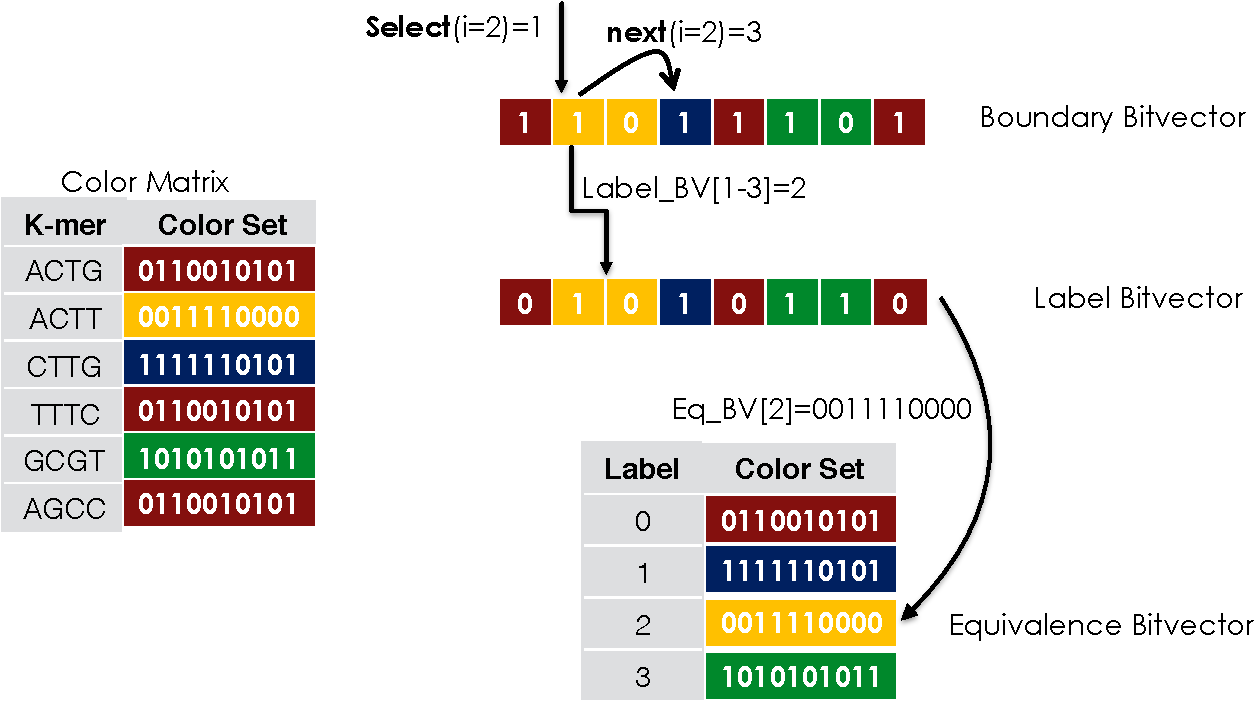
\includegraphics[width=\textwidth]{figs/cdbg-cropped}
  % \resizebox{0.80\linewidth}{!}{
  %   \ifpdf
  %     \input{cdbg-rep.pdf_tex}
  %   \else
  %     \input{cdbg-rep.eps_tex}
  %   \fi
  %   }
  \caption{
    The representation of color information in \system. The ``Color Matrix'' at
    the top represents $6$ distinct $4$-mers, each assigned a color set. $3$ of
    these $4$-mers (ACTG, TTTC, AGCC) have the same color class, labeled $0$,
    and the other $3$ (CTTG, ACTT, and GCGT) each have color classes labeled
    $1$, $10$, and $11$ respectively. To retrieve the color set for a \kmer, we
    first perform select on the boundary bit vector (BBV) using rank $r$ of the
    corresponding edge (\kmer). This returns the label's starting position, $i$.
    We then look for the next set bit BBV to find the label's ending position,
    $j$. Then, we fetch the label at indices $i$ to $j$ in label bit vector
    (LBV). Finally, we lookup the label $l$ in the equivalence class table (ECT)
    and return the color class corresponding to the label. A detailed
    explanation of the data structure and its construction is given in
    \Cref{design}.
  }
    \label{fig:cdbg-rep}
\end{figure}

In this section we first describe the design of \system. We then analyze the
space usage and provide a lower bound for the representation of sets of colors given
a ranking of \dbg edges. Finally, we discuss the \system implementation.

\subsection{~Design}
\label{design}

\system's compact representation of color information is based on two particular
observations. First, it is often the case that many of the \kmers in a \cdbg
share the same set of colors. More formally, we define an equivalence relation
$\sim$ over the set of \kmers in the \dbg. Let $\cfun{\cdot}$ denote the
function that maps each \kmer to its corresponding set of colors. We say that
two \kmers are color-equivalent (i.e., $k_1 \sim k_2$) if and only if
$\cfun{k_1} = \cfun{k_2}$. We will refer to the set of colors shared by the
\kmers related by $\sim$ as a \defn{color class}. If $C$, the number of input
colors, is large, it is often the case that the number of distinct color classes
is far less than the number of possible color classes (which is bounded above by
$\min(N,2^C)$).

Second, it is often the case that the frequency distribution of color classes
is far from uniform.  Hence, it will often be useful to record a frequently
occurring color class using a short description (i.e., a small number of bits)
while reserving larger descriptions for less frequent color classes.

%Put another way, both of these observations can be summarized in
%that we expect $H(X_c)$---the entropy of the color class---to be low (i.e., the
%expected value of the information available in each color class is low or
%order-$0$ entropy).

The design of \system is motivated by the above observations. Instead of storing
the color set for each \kmer separately, \system stores each distinct color
class only once and assigns to each distinct class a label (which, practically,
is much smaller than the unary encoding of the color class itself).
%
%\fatemeh{Furthermore, by replacing the fixed-length label with a variable-length
%one \system leverages the skewness property of distribution of \kmers across
%distinct color sets to save even more space.}
%
%starting from label 0 with 1 bit length. 
%
It then stores, for each \kmer, the label of the color class to which it
belongs. 
%
%Considering the skewed distribution of color class frequencies, this data
%structure can practically be much more efficient compared to the unary encoding
%of the color sets for each \kmer.

The approach we use to assign variable-length labels to color classes is similar
in spirit to the construction of a Huffman code, where the message is a string
of color class symbols. However, we do not build a prefix code, and instead opt
to store an additional bit vector to allow the efficient selection of an
arbitrary label from the list. We generate the labels according to the following
procedure. We first sort, in descending order, all the color classes based on
their frequency (i.e., the number of \kmers in this color equivalence class). We
then assign labels to each color class starting from the class with the largest
cardinality, so that the color class represented by the most frequent label will
have the shortest label length etc.

%The approach we use to assign variable-length labels to color classes is
%similar in spirit to the construction of a Huffman code, where the message is a
%string of distinct color sets (each representing symbol of a color class) and
%frequency of each symbol is frequency of each color class or in other words
%number of distinct \kmers observed with that color set. However, we do not
%build a prefix code, and instead opt to store an additional bit vector to allow
%the efficient selection of an arbitrary label from the list. We generate the
%labels according to the following procedure. We first sort, in descending
%order, all the color classes based on their frequency (i.e., the number of
%\kmers that display this color class). We then assign consecutive numbers as
%labels to each color class starting from the color class displayed by the most
%\kmers, so that the color class appearing as the most frequent label will have
%the shortest label length (which is 1 bit) etc.

The color class representation in \system has three components. \system stores
the mappings between labels and color classes in an \defn{equivalence class
  table (ECT)}. As labels are assigned sequentially, this is simply an array of
bit vectors encoding the corresponding color sets. Apart from the equivalence
class table, \system maintains two bit vectors, a \defn{boundary bit vector
  (BBV)} and a \defn{label bit vector(LBV)}.

All color classes are stored in the equivalence class table (with their
corresponding labels implicitly being their position). However, we now need to
store a mapping from \kmers to the variable-length labels. \system stores
variable-length labels corresponding to each \kmer in the label bit vector. The
labels are stored in the order in which \kmers are stored in the \dbg
representation. Specifically, the \kmers are stored in the rank order induced by
\boss. However, since these labels are variable-length, we can not directly read
the label corresponding to the \kmer of a specific rank, since we do not know
where such a label begins or how long it is.

To address this, \system maintains another bit vector --- the boundary bit
vector (BBV) --- to mark the boundary of each variable-length label in LBV. The
BBV is the same size as the LBV and has a bit set
to 1 at each index where a new label starts in the LBV. Thus, the starting
position for the label corresponding to the $r$th \kmer can be obtained by
issuing a \select{(r)} query on BBV, and the length of this label can be
obtained by simply scanning BBV until we encounter the next set bit.

\Cref{fig:cdbg-rep} shows how the color classes are represented in \system. To
perform a query for the color class corresponding to a \kmer in the \cdbg, we
first get the rank $r$ of the \kmer in the \dbg. We then perform a select
operation using $r$ on BBV. The result of the select operation $i$ is the start
index of the label of the color class in LBV to which the \kmer belongs.
%
To find the length of the label we determine the index $i'$ of the next bit set
in BBV using the \textsc{tzcnt} instruction.
%
\textsc{tzcnt} returns the number of trailing zeros in its argument. If $B$ is a
12-bit vector such that $B[0,11]=$\texttt{110010100000} then
$\textsc{tzcnt}(B)=5$.
%
%another select operation \fatemeh{we don't do that anymore} using $r+1$ to find
%the start of the next label. The difference between the start of the next label
%$i'$ and $i$ is the length of the label in the label bit vector. 
%
Using $i$ and $i'$ we retrieve the label from LBV, and using
the label we lookup the corresponding color class in ECT.
%
We also note that, as we never have $> 2^{64}$ distinct \kmers in practice, and
number of distinct labels is at max equal to the number of distinct \kmers (when
each \kmer has a unique label), then we never have $> 2^{64}$ labels. Hence, we can
always represent a label using a single machine word. Consequently, we will
always reach the next set bit in the LBV after scanning at most a single machine
word when starting from current label. This ensures we need only issue a single
\textsc{tzcnt} instruction per label decoding call.


\subsection{~Space analysis}
\label{system-space-bound}

The color class representation in \system is entropy compressed, i.e.,
the space is bounded by the entropy ($H(X_c)$) of the color class distribution. 
For a dataset in which number of \kmers belonging to each distinct color class are
similar, the entropy of the color class distribution will be high. On the other
hand, if most of the \kmers in a dataset belong to a small number of distinct
color classes, the entropy of the color class distribution will be low.

\begin{lemma}
  The size of each color class label is bounded by $\log_2{M}$ bits, where
  $M$ is the total number of distinct color classes. For a dataset with $N$
  distinct \kmers coming from $C$ input samples (i.e., colors), we have that $M
  \leq \min(N,2^C)$.
  \label{label-size-bound}
\end{lemma}

%\prashant{I have changed the wording in theorem 1. I don't know if it's better or worse.}

\begin{theorem}
Given an ordering of edges (or \kmers) in a \dbg, the space needed by \system to
represent a set of colors attached to each edge is $\order{MC+N H(X_c)}$ bits,
where $M$ is the number of distinct color classes, $C$ is the number of colors,
$N$ is the number of distinct \kmers, and $H(X_c) = -\sum_{i=1}^{M} P(x_i)\log
P(x_i)$ is the entropy (i.e., order-$0$ or Shannon's entropy) over random
variable $X_c$, which distributed according to the frequency distribution of the
color classes.
%$H(X_c)$ is the entropy of the color class distribution. 
\label{space-bound} \end{theorem}

\begin{proof}
%
The space needed by \system can be analyzed as follows. There are three bit
vectors in \system, the equivalence class table, label bit vector, and boundary bit
vector. To store an equivalence class table containing $M$ distinct color
classes each having $C$ colors we need $MC$ bits. To store a label bit vector
(as stated in \Cref{label-size-bound}), for $N$ \kmers, where each label
corresponds to one of the $M$ distinct color classes, takes $N\log_2{M}$ bits.
However, as explained in \Cref{design}, in \system we assign (optimal) variable-length
labels based on the frequency of color classes. Therefore, the space needed to
store the label bit vector is dependent on the $0$th-order entropy of the color
class variable, $H(X_c)$, and the size of the label bit vector is upper bounded
by $N\log_2{M}$.  The boundary bit vector has the same number of bits as the
label bit vector. 
%
\end{proof}

%%
% This seems redundant
%%
%As explained in \Cref{space-bound}, the space required to represent the label
%bit vector in \system depends on the entropy of the color class distribution.
%For a uniformly-random distribution the space would be high compared to a skewed
%distribution. The boundary bit vector contains the same number of bits as the
%label bit vector.


\subsection{~Lower bound for color representation}

%\fatemeh{I think we need a few sentences here to say we divide the space bound
  %to equivalence table space and label/boundary bit vectors and explain we are
  %already succinct regarding storing the equivalence table with space bound of
  %$\order{MC}$. Then say we now prove why we are also succinct regarding
  %label/boundary bit vectors with practical space of $\order{NH(X_c)}$}

We now provide a lower bound to store a color class representation for a set of
edges in a \cdbg. In the color class representation, the equivalence class table
takes $MC$ bits to store $M$ bit vectors each having $C$ bits, which is
optimal. The other two bit vectors, the boundary and label bit vector, map \kmers
given an ordering in the \dbg to their corresponding color classes. The theorem
below gives the lower bound to store such a mapping.
 
\begin{theorem}
%
  The lower bound to represent a mapping from an ordered list of \kmers in a
  \dbg to a set of color classes is $\log_2{(M^{N-M} \cdot M!)}$ bits, where
  $M$ is the number of distinct color classes, $N$ is the number of edges, and
  for a dataset with $N$ distinct \kmers coming from $C$ input samples (i.e.,
  colors), we have that $M \leq \min(N,2^C)$.
%
\end{theorem}

\begin{proof}

We can analyze the lower bound using a counting argument. We count the number
of ways to map a set of $M$ distinct color classes to a set of $N$ edges. The
space required to store the color class representation should be less than or
equal to the space required to store these mappings.

Edges can be mapped to color classes using a surjective (onto) function. Thus,
we wish to count the total number of surjections from $M$ color classes to $N$
edges. Rather than counting this number exactly, we instead provide a lower bound.
First, we must ensure that each of the $M$ color classes maps to at least one
edge --- so, we select a set of $M$ edges and label each with a distinct color
class. There are $M!$ ways to assign $M$ color classes to a set of $M$ edges. We
will then allow the remaining $N-M$ edges to be colored in any possible manner.
We can assign $M$ colors to $N-M$ edges (the remaining number) in $M^{N-M}$
ways. Therefore, the total number of different mappings is bounded below by $M^{N-M}
\cdot M!$. To be able to represent each such mapping, and distinguish it from
the others, we need at least $\log_2{(M^{N-M} \cdot M!)}$ bits.
\end{proof}

The lower bound can be expanded using Sterling's approximation as
\[
(N-M)\log_2{M} + M\log_2{M} - 0.44M + O(\log_2{M}),
\]
which, ignoring the
additive term $\order{\log_2{M}}$, is greater or equal to $N\log_2{M} - 0.44M$. Given the range of
$M$ (i.e., $1 \leq M \leq N$), $N\log_2{M}$ always dominates the lower bound.

Now, we show that the space needed by \system to store the variable-length
labels assigned to color classes is equal to the lower bound. As explained in
\Cref{label-size-bound}, the upper bound to store any label is $\log_2{M}$ bits,
and for $N$ edges, it is given by $N\log_2{M}$ bits.  \system also stores a
boundary bit vector which has the same number of bits as the label bit vector.
Therefore, the space required to store the label mappings is strictly $\leq
2N\log_2{M}$. Note that the extra overhead to store the metadata to perform a
select operation in constant time on the boundary bit vector is bounded by
$o(N)$, where $N$ is the numbers of bits in the bit
vector~\cite{GonzalezGrMa05}.

However, \system's representation of color classes is entropy compressed (see
\Cref{design}) and the space required depends on the entropy of the color class
distribution. For a highly skewed distribution, the entropy is low and the space
required to store labels is much smaller than $N\log_2{M}$ bits. On the other
hand, when the distribution is near-uniform, i.e., the entropy is high, \system
makes all labels to be $\log_2{M}$ bits and dispenses with BBV. Therefore, the
space required by \system is always smaller than or equal to the lower bound.

%\fatemeh{Here we are proving ds <= O(Z) while for succinct we should prove ds
%= Z + o(Z). The first is the proof for compact. So one idea we discussed with
%Robp is to remove $\order{}$ from $\order{N\log_2{M} -/+ blabla}$ and consider
%it as $Z'$ which is itself a lower bound on Z ($Z' = Z + o(Z)$). Then we prove
%ds = $Z' + o(Z') = Z + o(Z) + o(Z + o(Z)) = Z + o(Z)$}


\subsection{~Implementation}

\tikzsetnextfilename{plant-eq-class-dist}
\begin{figure}[h]
\centering
\begin{tikzpicture}[scale=0.8]
  \begin{axis}[
    ybar,
    %x=2pt,
    %height=6cm,
    bar width=3pt,
    xtick=data,
    scaled ticks=false,
    ymode=log,
    ymin=0,
    ylabel={\#\kmers in each equivalence class},
    xlabel={Equivalence class labels},
    legend style={at={(1.05,0.63)}, anchor=north west},
    nodes near coords align={vertical},
  ]
    \pgfplotstableread{data/plant-eqDist-1pass}\loadedtable;

      \addplot[color=teal, fill=teal] table[x=x_0, y=y_0] {\loadedtable};
      \addplot[color=olive, fill=olive] table[x=x_0, y=y_1] {\loadedtable};
      %\addplot[color=teal, fill=teal] table[x=x_0, y=y_2] {\loadedtable};
      \legend{Color class dist. in $1$-pass,Color class dist. in $2$-pass}
    \end{axis}
\end{tikzpicture}
    \caption{
    Distribution of \kmer frequencies across equivalence class labels in \system
    after $1$-pass and $2$-pass algorithm on plant dataset
    \Cref{tab:datasets-info}. The $2$-pass algorithm assigns the smallest label
    to color class with maximum number of \kmers. The distribution in $2$-pass
    algorithm is monotonically decreasing. 
  }
      \label{fig:plant-eq-class-dist}
\end{figure}

\subparagraph{Considerations due to the underlying \dbg representation} We recall here that we make use of the BOSS representation of the underlying \dbg topology. To build the BOSS representation, \kmer counting is first performed using KMC2~\cite{Deorowicz15KMC}, canonicalizing \kmers during counting. Though the BOSS representation inserts both forward and reverse complement \kmers into the graph, it associates only a single color vector with this pair.  Moreover, BOSS creates ``dummy'' edges (real \kmers prepended or appended with \$) to allow encoding \kmers that appear near terminal nodes in the \dbg. In the \cdbg these dummy edges are assigned the empty color set. All of this information is encoded by both \vari and \system. However, as we discuss in more detail in~\Cref{sec:conclusion}, the \system representation can work with any \dbg representation that can assign distinct ranks to each \kmer in the \dbg. Thus, we would expect this encoding scheme to work well with, e.g., a \dbg representation based on minimum perfect hashing of the
\kmers~\cite{drezen2014gatb}.
%\fatemeh{We should note that as BOSS counts a \kmer and its reverse complement as two distinct \kmers, we also count them as two different \kmers.}

\subparagraph{Storing bit vectors.} In \system, we use bit vector implementations
from the SDSL library~\cite{sdsl} to store the three bit vectors from
\Cref{fig:cdbg-rep}. We use the $rrr\_vector$ implementation from SDSL to store
the equivalence class table and boundary bit vector, and the $bit\_vector$ implementation
from SDSL to store the label bit vector.

The $rrr\_vector$ of SDSL is an implementation of \rrr encoding~\cite{RamanRaRa02}. \rrr
encoding is an entropy compressed encoding and also supports constant time rank
and select operations on the compressed bit vector.  The space reduction depends
on the entropy of the bit vector. For high entropy bit vectors, the compression
is not noticeable and in fact ``negative'' in some cases because of the extra
metadata overhead to support rank and select operations.

The equivalence class table and boundary bit vector often have fairly low
entropy, and can be compressed efficiently using RRR encoding. However, the
label bit vector often has high entropy, and compressing it using \rrr encoding
is not effective. In our representation, the average order-$0$ entropy of the
label bit vector for four different datasets is $0.94$. This is a quite high,
and hence we did not see any reduction in the space using \rrr encoding.
However, for the other two bit vectors, the order-$0$ entropy is lower (e.g.,
for boundary bit vector the average entropy over same four datasets is $0.56$)
and, in practice, we achieve a considerable space reduction using RRR encoding.

\subparagraph{Construction.} We use a $2$-pass algorithm to construct the three bit vectors. In the first pass, we read the color matrix, compute the distinct color classes, and count the frequency of each class. Once we have the frequency information, we sort color
classes in descending order based on their frequency. We then assign labels to
color classes starting from zero. In the second pass, we read the uncompressed
color matrix again, and add the label of each \kmer to the label bit vector.
While building the label bit vector, we also build the boundary bit vector by
storing a $1$ at every index where a new label starts in the label bit vector.
The labels are stored in the same order as the \kmers in the \boss
representation.

To reduce the space required for the labeling even further, we implemented our label
encoding in the following way. Every time that the label size increases from $x$
bits to $x+1$ bits, we restart the counter of that label in label bit vector to
$0$. For example, we store $0$ and $1$ for labels $0$ and $1$ respectively,
then we store $00$, $01$, $10$ and $11$ for labels $2$, $3$, $4$ and $5$
respectively. For label value $6$ we again restart the counter to $0$ and store
$000$ to represent $6$ in the label bit vector, etc. Later, when we want to retrieve
the actual value of a label, we first recover the stored label $l'$ from the label
bit vector and then calculate the actual label $l$ using the equation $l = l'
+ 2^{d}-2$ where d is length of label $l$ in bits.

As explained in \Cref{system-space-bound}, the $2$-pass algorithm minimizes the
space used to represent color class labels by sorting the classes based on their
frequencies and assigning labels to color classes to minimize the length of the
resulting code path, similar to Huffman coding. However, one could also imagine
assigning labels to color classes as we see them in the order \kmers appear in
the \boss representation. This way, we can construct all three tables in a single
pass (i.e., a $1$-pass algorithm).

However, as shown in \Cref{fig:plant-eq-class-dist}, this $1$-pass algorithm can
end up assigning long labels to frequent \kmers, and hence produce poor (i.e.,
large) encodings. However, the $2$-pass algorithm always assigns labels
according to the corresponding frequency distribution of the color classes.
Sometimes, the $1$-pass algorithm does well, but we chose to adopt the $2$-pass algorithm
in \system. 

\section{~Evaluation}

\begin{table}
  \begin{center}
    \begin{tabular} {| l | c c c|}
    \hline
      Datasets & \# of edges & \# of colors (samples) & \# of distinct color classes \\
      \hline
      \ecoli 10 & 28,273,951 & 10 & 479\\
      \ecoli 1000 & 157,737,064 & 1000 & 2,669,157 \\
      \ecoli 5598 & 435,705,390 & 5598 & 7,000,715\\
      \ecoli 1000 (k=63) & 258,893,268 & 1000 & 2,530,253\\
      Plant & 2,520,140,426 & 4 & 16 \\
      Beef safety & 97,096,576,010* & 87 & 623,022,532\\
      Human transcriptome & 159,441,804* & 95,146 & 340,762\\
      \hline
      % &  e-coli 10 & e-coli 1000 & e-coli 5598 & Plant & Beef Safety \\
      %Num. of Edges &  & 157,737,064 & 435,705,390 & 2,279,614,458 & \\
      %Num. of Colors & 10 & 1000 & 5598 & 4 & 87 \\
    \end{tabular}
  \caption{
    The number of edges (include \kmers and dummy edges in the BOSS
    representation), samples and color classes for different datasets used in
    the experiments. $k = 32$ unless otherwise specified. \small
    *\# of edges excluding dummies.
}
\vspace{-2.5em}
  \label{tab:datasets-info}
\end{center}
\end{table}

\begin{table}
\begin{center}
\begin{tabular} {| l | c c| c c|}
\hline
Datasets & \multicolumn{2}{c|}{Construction Time (secs)} & \multicolumn{2}{c|}{Bubble Calling Time (secs)} \\
\cline{2-5}
& \vari & \system & \vari & \system \\
\hline
\ecoli 10 & 44 & 31 & 344 & 366\\
\ecoli 1000 & 340 & 270 & 2,610 & 2,356\\
\ecoli 5598 & 3,141 & 4,021 & 8,796 & 8,201\\
%\ecoli 1000 (k=63) & 323 & 257 & 3,971 & 7,546\\
\plant & 108 & 339 & 47,040 & 48,537\\
\beefsafety & 15,378 &  30,478 & NA & NA\\
Human transcriptome & 13,961 & 30,804 & NA & NA\\
\hline
\end{tabular}
\caption{
  Construction and bubble calling time for \system and \vari for different
  datasets. 
}
\vspace{-2.5em}
\label{tab:time}
\end{center}
\end{table}

In this section we evaluate \system, and compare it to \vari~\cite{Muggli17}, a
state-of-the-art \cdbg representation. We evaluate both systems in terms of
space and running time. We address the following questions about the performance
of \system: How does \system compare to \vari in terms of the space required to
represent color information?; How does \system compare to \vari in terms of the
construction time?; How does \system compare to \vari in terms of typical
queries (e.g., in bubble calling)? We are particularly concerned with ensuring
that \system produces small encodings of the color information and remains
practically efficient to query.

\subsection{~Experimental setup}

To answer the above questions, we perform two different benchmarks. First, we
evaluate the time taken to construct the color class representation. The
construction time is the time taken to construct the color class representation
from a list of color classes stored in the order of the edges in the \dbg (this
is the same input used by \vari). During construction, we adopt a two-pass
algorithm. In the first pass, we use a sparse hash-table to determine the distinct
color classes and the cardinality of each such class.

We note that the space taken in this first pass is within a small constant
factor of the final space required by the final ECT table itself, since we need
only store each color class once in the hash table (as a key), and store the
associated count (a machine word) as the value.  Thus, the memory required by
this first pass is almost always a small fraction of the total memory usage 
of the construction algorithm.

Given this information, we know exactly the number of bits that will be required
to store the label and boundary vectors. In the second pass, we fill in both the
label and boundary vectors and then save all three structures to file. As with
most succinct representations, the space required for our data structure in
memory and on disk is almost the same (as the two-pass algorithm allows us to
allocate only the space we need for our final representation). The construction
time recorded here does not include (for either \system or \vari) the time taken
to build the \dbg and color list corresponding to edges in the \dbg (since this
is the same for both methods).

We also report the space needed by both \system and \vari to store the color class
representation on disk. We do not include the space needed to represent the
actual \dbg in our space comparisons because both \system and \vari use \boss
to store the actual \dbg, and the \boss representation itself tends to take less
space than the color information.

Second, we evaluate the time taken to perform the bubble calling benchmark as
described in~\cite{MuggliBoNo17}, using both the \vari and \system
representations. Finding bubbles in a \cdbg enables one to detect regions in the
\dbg where different samples (i.e., colors) diverge from each other. As
originally suggested by Iqbal et al.~\cite{Iqbal2012Novo}, such algorithms can
form the basis for analyzing certain types of genetic variants in populations of
genomes. We note that we adopt the exact bubble calling algorithm implemented in
\vari, and the only variable being altered in our bubble-calling benchmark is
the data structure being used to determine the set of colors present for each
\kmer. Since \vari and \system are both built upon the \boss representation,
which is based on the edge-centric view of \dbg, they consider \kmers as edges
in the \dbg, meaning that each edge is associated with a \kmer, and its
corresponding rank and color set. Briefly, the bubble calling algorithm takes as
input a pair $c_1,c_2$ of colors and traverses edges in the \dbg to find bubbles
in which the edges in one sub-path are colored with $c_1$ and the edges in the
other sub-path are colored with $c_2$ (see~\cite{MuggliBoNo17} for further
details).

For all experiments in this paper, unless otherwise noted, we consider the \kmer
size to be $32$ to match the parameters adopted by Muggli et
al.~\cite{MuggliBoNo17}. We carry out these benchmarks on a number of datasets
as described in \cref{subsec:data}. The time reported for construction and
bubble calling are averaged over two runs, and the time is measured as the
wall-clock time using the \texttt{/usr/bin/time} executable. All experiments
were performed on an Intel(R) Xeon(R) CPU (E5-2699 v4 @2.20GHz with 44 cores and
56MB L3 cache) with 512GB RAM and a 4TB TOSHIBA MG03ACA4 ATA HDD running ubuntu
16.10, and were carried out using a single thread. We note that, while the
construction of the color set representation in \system (and \vari) are serial
operations, queries are trivially parallelizable, as each label can be queried
and decoded independently.

\subsection{~Data}
\label{subsec:data}

We run our benchmarks on the datasets mentioned in \Cref{tab:datasets-info}.
The first three datasets, 
%All three datasets 
\ecoli, \plant, and \beefsafety are slight variants of those used for
evaluation in \vari~\cite{MuggliBoNo17}. Each of these data sets exhibits
different characteristics in terms of the number of \kmers, the number of input
samples (i.e., colors) and the homogeneity of the underlying samples (i.e., how
different are the \dbg for each of the individual samples).
%
The first dataset consists of the assemblies of 5,598 different strains of
\ecoli obtained from GenBank~\cite{o2015reference}. Here, each ``color''
represents a specific \ecoli assembly. Since these assemblies are from
different strains of the same species, they exhibit a small degree of
heterogeneity. In other words, a large fraction of the union \dbg is expected
to occur in all samples.

To evaluate the scalability of \system when primarily changing the underlying
number of input colors, we have evaluated three variants of the \ecoli dataset.
These consist of a dataset containing only 10 different strains, another
containing 1,000 different strains and the final containing all 5,598 strains.
We also performed experiments with \kmer size to be $63$ for \ecoli 1000
dataset to evaluate the space usage for higher \kmer sizes.


%All these experiments are conducted on set of \kmers derived from
%the data with $k=32$. In addition to that, to evaluate the effect of k in for
%\kmers in the space required by \system we ran it \kmers with $k=63$ from
%\ecoli 1000.

%Using all \ecoli assembly samples we will have \kmers from 5,598 different
%colors. To evaluate the effect of varying number of colors on storage and
%performance of \system, we design three different experiments on \ecoli data
%running all steps of the process on the first 10, 1000, and then all 5,589
%\ecoli samples. 
The second dataset (i.e., \plant) consists of the genome assemblies of four
different plant species. Hence, this dataset contains only four colors, but has
more than $\approx2$ billion distinct \kmers. The plant species considered are,
\fnurl{\textit{A}. \textit{thaliana}
}{ftp://ftp.ensemblgenomes.org/pub/plants/release-34/fasta/arabidopsis_thaliana/dna/Arabidopsis_thaliana.TAIR10.dna.toplevel.fa.gz}~\cite{swarbreck2008arabidopsis},
\fnurl{Corn}{ftp://ftp.ncbi.nlm.nih.gov/genomes/all/GCF/000/005/005/GCF_000005005.1_B73_RefGen_v3/GCF_000005005.1_B73_RefGen_v3_genomic.fna.gz}~\cite{schnable2009b73},
\fnurl{Rice}{http://rice.plantbiology.msu.edu/pub/data/Eukaryotic_Projects/o_sativa/annotation_dbs/pseudomolecules/version_7.0/all.dir/all.con}~\cite{tanaka2008rice},
and
\fnurl{Tomato}{ftp://ftp.solgenomics.net/tomato_genome/assembly/build_2.50/SL2.50ch00.fa.tar.gz}~\cite{causse2013whole}.
%
These genomes exhibit considerable diversity and heterogeneity. Given the
diverse regions in the \cdbg, this dataset is a good candidate for the bubble
calling benchmark. Further, Muggli et al.~\cite{MuggliBoNo17} found that this
was the only of the three original datasets on which they were able to construct
the original \texttt{Cortex} representation of the \cdbg. They validated
\texttt{Cortex} produces the same bubble calls as \vari ~\cite{MuggliBoNo17}
(which, of course, produces the same bubble calls as \system).
%
For more detailed analysis of \texttt{Cortex}'s construction and processing time
and space on this dataset, please refer to~\cite{MuggliBoNo17}.
%
%among different samples that later will be critical for time evaluation in
%bubble finding process as there will be a lot of branching in \dBG and hence a
%lot of access queries for pair of \kmer and color on each branch. 
%

The third dataset, \beefsafety, is considerably different from the prior data.
Instead of the input samples consisting of assembled genomes, they consist of
87 metagenomic samples sequenced from cattle in the commercial process of beef
production~\cite{noyes2016resistome}. Hence, this dataset yields a considerably
larger and more complex \dbg since it is built upon many un-assembled (and
non-error-corrected) reads. Thus, the \dbg will encode portions of the relevant
metagenomes as well as the effects of sequencing errors. This dataset also has
many more \kmers than the others, $\approx97$ billion. It exhibits a large
degree of heterogeneity and an intermediate number of input colors (87).
%
%is a doubly huge dataset with total amount of 97,096,576,010 \kmers and
%considerable number of colors (87) and heterogeneity which provides a good
%practical example to evaluate time and space of \system compared to
%state-of-the-art colored \dBGs, \vari. 
%

In addition to the three datasets used in the \vari paper, we also consider
building the \cdbg on the \fnurl{human
transcriptome}{ftp://ftp.sanger.ac.uk/pub/gencode/Gencode_human/release_26/gencode.v26.pc_transcripts.fa.gz}
(Gencode v26 protein coding transcripts)~\cite{Harrow2012}. Here, we consider
each transcript as an individual sample (i.e., a distinct input color). This
data consists of $\approx95,000$ colors, but only $\approx159$ million \kmers.
Hence, this dataset will give an idea about how the representations
will perform when the number of colors becomes very large (though the number of
distinct color classes remains orders of magnitude smaller than the number of
\kmers). Further, we note that this dataset highlights some of the similarities
between the color class encoding adopted by \system and the \kmer-based
equivalence class decomposition adopted by certain transcript quantification
methods (e.g.~\cite{PatroSailfish:2014}).

%The fourth dataset illustrates another use case for \cdbg tools other than
%metagenomic analysis. This dataset is human transcriptome in which we consider
%each transcript as an individual sample, so that the \cdbg built upon this
%dataset has as many colors as transcripts.

%\footnote{ftp://ftp.ensemblgenomes.org/pub/plants/release-34/fasta/arabidopsis_thaliana/dna/Arabidopsis_thaliana.TAIR10.dna.toplevel.fa.gz}
%,
%\fnurl{Corn}{ftp://ftp.ncbi.nlm.nih.gov/genomes/all/GCF/000/005/005/GCF_000005005.1_B73_RefGen_v3/GCF_000005005.1_B73_RefGen_v3_genomic.fna.gz},
%Rice
%\footnote{http://rice.plantbiology.msu.edu/pub/data/Eukaryotic_Projects/o_sativa/annotation_dbs/pseudomolecules/version_7.0/all.dir/all.con}
%and Tomato \footnote{
%ftp://ftp.solgenomics.net/tomato_genome/assembly/build_2.50/SL2.50ch00.fa.tar.gz}

\subsection{~Performance}

\Cref{tab:time} shows the time taken by \system and \vari to construct the color
class representation for different datasets. \system uses a $2$-pass algorithm
to construct the color class representation, and hence the construction time is
dominated by the steps to read the color list file twice. For small datasets
like \ecoli $10$ and \ecoli $1,000$, the input file size is small and does not affect
the overall construction time compared to \vari. However, for large datasets
like \plant and \beefsafety, the time to read the color file twice dominates the
construction time and \system is $1.9\times$---$3\times$ slower. We note that
this time can be considerably reduced by avoiding the uncompressed color matrix
representation currently used upstream of \system and \vari, and integrating
determination and encoding of the color classes into the \dbg construction
directly. However, this is outside the scope of the current paper.

\paragraph*{~Space}\Cref{tab:space} shows the space usage of \system and \vari
for the different datasets we consider. Among these data, there are a range of
characteristics in terms of the number of \kmers, the number of colors, and the
complexity and heterogeneity of the \dbg. We find that, for all datasets,
\system requires less space to store the color information than \vari.  The
magnitude of the improvement depends on the number of distinct equivalence
classes and their distribution, but is as large as $\sim 20\times$.  We see the
same trend with higher values of \kmer sizes.

%\fatemeh{Even changing $k$ to higher value doesn't change the trend.}

In particular, \system's space usage is particularly impressive for datasets
with a large number of input colors but a relatively small number of distinct
\kmers. In this case, we usually find that the number of distinct color classes
is very small compared to the universe of possibilities, and so each label can
be encoded in much fewer than $C$ bits. However, the space \vari consumes
depends greatly on the sparsity of the color matrix. The color matrix itself
grows rapidly as the number of \kmers and colors increases, but \vari's
compression mechanism (Elias-Fano encoding) is very effective if the color
matrix is sparse (e.g., each \kmer is labeled with only a small subset of
colors). This is exactly the case for the Human transcriptome, where the color
matrix has an entropy of $\sim 0.0004$ (compared to \ecoli 5,598 and \ecoli
1,000 with entropies of $\sim 0.16$ and $\sim 0.34$ respectively). Thus, in the
\ecoli dataset, \vari can save space up to a factor of $\sim 5$ compared with
the uncompressed representation, while in the Human transcriptome it can save a
factor of $\sim 2,150$ because of the low entropy of the color matrix. \system
does well in all experiments, even when the number of input colors is small
(e.g., in the \plant dataset). \system achieves the most impressive compression
when the color class distribution has low entropy and the number of color classes
is small relative to the upper bound.
In such cases, the entropy compressed representation of \system is able to
represent a large fraction of all labels using a very small number of bits.
%\fatemeh{
%while because of high entropy in color matrix, \vari's space increases as a result of negative compression. 
% --> This low entropy in color class distribution and high entropy in color matrix might be a little bit confusing but really interesting to talk about.} 


\begin{table}
\begin{center}
\begin{tabular} {| l | c c c|}
\hline
Datasets & 
uncompressed color matrix & \vari & \system \\
\hline
\ecoli 10 & 34 & 58 & 20 \\
\ecoli 1000 & 18,804 & 8,848 & 475 \\
\ecoli 5598 & 290,761 & 58,718 & 2,938 \\
\ecoli 1000 (k=63) & 185,669 & 8,872 & 637\\
\plant & 1,202 & 1,603 & 497 \\
\beefsafety & 1,007,009 & 210,998 & 144,564 \\
Human transcriptome & 1,808,435 & 841 & 817 \\
\hline
\end{tabular}
\caption{
  The space required by \system and \vari to store the color class
  representation for different datasets. The first column shows space required for the uncompressed color matrix ($N \times C$ bits).
  All space is reported in MB. $k = 32$ unless otherwise specified.
}
\vspace{-3.5em}
\label{tab:space}
\end{center}
\end{table}

%Based on the design of our data structure we would expect to see an order of
%magnitude improvement in storage as number of colors increase. We expect to do
%as well as \vari in case of 10 samples of \ecoli as a small dataset with few
%colors and do much better regarding space in case of considering all 5,598
%samples. table \ref{tb:space} shows changes of storage while changing number
%of colors. As shown in table \cref{tb:space} \system improves space when
%number of colors increase from taking 16 times less space in \ecoli with 1000
%samples to 26 times in full \ecoli dataset compared to \vari. 

%Another interesting result is the huge amount of space improvement we see in
%\plant dataset although it has just four colors which implies that \system not
%only works better in terms of increasing number of colors but also when we have
%a huge amount of \kmers. While in \vari, they keep four bits per each \kmer in
%\plant dataset (one bit for each color and hence four bits for four colors),
%but still replacing that with two bits for the first two most frequent color
%sets in \system can still save a lot of space when we have a considerable
%amount of \kmers even with the overload of saving equivalence table.

\paragraph*{~Bubble calling} \Cref{tab:time} shows the time taken by \system and \vari to perform the bubble
calling benchmark on different datasets. We run the bubble calling benchmark on
the \ecoli and \plant datasets (as in the \vari paper). We note that the current
bubble calling algorithm is too slow to run on the Beef safety data set (the
time in~\cite{MuggliBoNo17} was estimated at $>3,000$ hours). It is possible,
however, that optimizations to the underlying algorithm might lift this
restriction. We also did not perform bubble calling on the human transcriptome
dataset as here, we were unable, given the resources on our server, to even run
the \dbg construction to completion. Specifically, due to the large amount of
external memory that \vari uses to build the uncompressed color matrix and the
\dbg on these larger (either in terms of the number of \kmers, the number of
colors, or both) datasets (on order of Terabytes), we exhausted the available
disk space. For these datasets, to approximate the relevant sizes and
construction times, we produced a uncompressed color matrix that lists the
colors for each \kmer and its reverse complement, and we use this to build both
the \vari and \system color representations. While very similar to the full color
matrix that \vari would produce, this file is slightly different in that it does
not include entries for dummy edges (a detail of the \boss representation), and
the order of the color matrix rows can be different from what will appear in the
\boss representation. However, we still believe these numbers, provided in
\Cref{tab:datasets-info}, give a reasonable approximation of how the respective
methods would perform were we able to construct the \dbg completely.

For bubble calling, both representations require a very similar amount of time.
This is likely due, in part, to the fact that navigating the \boss
representation of the \dbg may be the performance bottleneck in the bubble
calling algorithm. Thus, both \vari and \system provide sufficiently fast access
to the color sets for each edge that they do not represent bottlenecks in this
regard.

\section{~Conclusion and Future Work}
\label{sec:conclusion}

In this paper, we propose an entropy-compressed, succinct data structure to
store the color information of a \cdbg. To represent the topology of the \dbg
itself, we adopt the \boss~\cite{BoweOn12} representation. However, we note
that, for our representation of the color sets, we only require that the
underlying \dbg representation is able to associate a unique rank between $0$
and $N-1$ with each edge. Hence, it is possible to use the \system
representation with other representations of the \dbg topology (e.g., those
based on minimal perfect hashing).

We demonstrate that the inherent skewness in the distribution of color classes
can be exploited to reduce the size of the color information. This allows
\system to represent the \cdbg, even for large datasets with many colors, in a
reasonably small space. In fact, for representing the color information itself,
we show that \system is succinct, and hence requires only $Z + o(z)$ bits where
$Z$ is the number of bits required by an information-theoretically optimal
representation.
%
Moreover, it may be possible for the color information stored in the equivalence
class table to be further compressed to reduce the space. For example, one could
imagine an encoding of color sets that takes advantage of their shared subsets,
e.g., storing the shared prefixes of membership vectors only once.
%
%It's also likely that reordering \kmers would reduce the entropy of the label
%vector and result in higher compression ratio. For example, \kmers appearing
%nearby in the \dbg have a higher probability of having the same color class.
%Reordering \kmers based on the \dbg traversal order can bring \kmers with same
%equivalence classes together and thereby increasing the skewness in the color
%information.

%\fatemeh{We keep each color once in ECT and later refer to that with its
%corresponding label for each \kmer and we prove that this representation is
%indeed succinct. However, we can still push compacting color representation in
%ECT even one step further to improve $o(z)$. For example we can exploit the
%color class similarity and instead of storing each set of colors for each color
%class, store shared prefixes of color classes only once. For current
%representation since we are dependent on \boss we cannot re-order \kmers, but if
%we switch to another representation of \dbg we might be able to save more space
%by re-ordering the \kmers to somehow have similar labels next to each other to
%enable more compression.}

While we have described here a system for efficiently representing the color
information in a \cdbg, our encoding scheme can be generalized to store any type
of attribute attached to the edges. For example, one could use the same (or a
related) scheme to encode information like the \kmer count or set of positions
associated with a given edge. Moreover, it will be interesting to explore how
multiple attributes could be efficiently stored simultaneously, and how
potential correlations between these attributes might be exploited. For example,
there may be natural extensions of similar coding schemes to the
\emph{compacted} \dbg, where one might also be able to take advantage of the
coherence in annotation (i.e., color or count information) shared among the
constiuent \kmers of a contig, allowing one to store only the information where
these annotations change during traversal.

Finally, in our current implementation, the input to the system is a color
matrix file generated by \vari. This implementation requires first building the
uncompressed color matrix, and then permuting the rows of this matrix along with
the edges of the \dbg during the \boss construction procedure. 
%
%
%\fatemeh{Since
%\system is dependent on color matrix as input, the building process } 
%
This process can require a large amount of space, as the uncompressed color
matrix can become extremely large (on the order of Terabytes for some of the
datasets we considered here). Consequently, in most cases, the construction
algorithm must resort to making extensive use of external memory (i.e., disk),
which increases building time and consumes a large amount of disk space.
However, we note that the \system representation can be built without direct
access to the uncompressed color matrix.

Specifically, the current \vari algorithm uses a mergesort-like approach to
construct the uncompressed color matrix, where the \kmers in each sample are
sorted lexicographically (independently), and the rows of the color matrix are
constructed one by one by asking for each \kmer, in lexicographic order, which
samples contain it. The working memory of this approach is very small compared
to the size of the full color matrix itself. One could imagine using the same
merge-based scheme to construct the \system representation directly. In the
first pass, the distinct color classes and a counter for each would be stored,
resulting in a small, sparse hash table rather than a large, uncompressed color
matrix. In the second pass, one would simply associate the relevant
labels, rather than uncompressed color vectors, with each edge. This would
vastly reduce the time and space required to construct the \cdbg.

%\fatemeh{In this
%way, we don't need the whole color matrix as an input to the construction
%process. Yet, we can build all the data structures in \system by just going over
%\kmer count files. In the first pass, we go over all \kmer files and build ECT
%with keeping the count of \kmers in each color equivalence class. In second
%pass, having total number of bits required to build LBT and BBV, we go over
%\kmer files another time and read off the \kmers and fill up the other two
%bitvectors. Hence, we save a large amound of space on disk by not keeping the
%color matrix and also the construction time won't be affected significantly as
%we are going over the same number of \kmers as the rows of color matrix in each
%pass.} 

Thus, in the future, we are interested in both incorporating the \system
representation more tightly inside the existing \vari codebase, as well as
pairing the \system representation with other compatible representations of the
\dbg topology.  

%\fatemeh{One of these representations is compacted \dbg in which
  %a \kmer and its reverse complement are represented with one id. This can help
  %improve the space \system takes by decreasing number of \kmers we have to
  %provide colorset for almost to half of number of unique \kmers calculated by
%\boss.}

\subparagraph*{Acknowledgments.}
We gratefully acknowledge support from NSF grant BBSRC-NSF/BIO-1564917. We also
thank Michael Bender and Robert Johnson for fruitful conversations and important
insight when performing this research. We would also like to thank Rayan
Chikhi for suggesting using auxiliary, rank/index-based storage for maintaining and
accessing annotations for each edge in a \dbg, and for useful feedback on an early
version of this manuscript.  Finally, we would like to thank the anonymous reviewers
for constructive feedback.
%\appendix 

%%
%% Bibliography
%%

%% Either use bibtex (recommended), 

%\bibliography{merged.bib}

%% .. or use the thebibliography environment explicitly



%\end{document}


\chapter{An Efficient, Scalable and Exact Representation of High-Dimensional Color Information Enabled via de Bruijn Graph Search}
\label{chap:mantis}


\section{Introduction}\label{sec:intro}

The \longcdbg (\cdbg)~\cite{IqbalCaTu12}, an extension of the classical
\dbg~\citep{pevzner2001eulerian,pevzner2001fragment,chikhi2014representation},
is a key component of a growing number of genomics tools. Augmenting the traditional
\dbg with ``color'' information provides a mechanism to associate meta-data,
such as the raw sample or reference of origin, with each \kmer. Coloring the \dbg
enables it to be used in a wide range of applications, such as large-scale sequence
search~\citep{mantis, Solomon2016Fast, Solomon2017Improved,
Sun2017Allsome, bradley2017real} (though some~\citep{Solomon2016Fast, Solomon2017Improved,Sun2017Allsome}
do not explicitly couch their representations in
the language of the \cdbg), population-level variation
detection~\cite{MuggliBoNo17, holley2016bloom, rainbowfish}, traversal and search
in a pan-genome~\cite{holley2016bloom}, and sequence
alignment~\cite{liu2016debga}. The popularity and applicability of the
\cdbg has spurred research into developing space-efficient and high-performance
data-structure implementations.

An efficient and fast representation of \cdbg requires optimizing both the \dbg and the
color information.  While there exist efficient and scalable methods
for representing the topology of the
\dbg~\cite{chikhi2012space,salikhov2014using,bowe2012succinct,chikhi2014representation,crawford2018practical,PandeyBeJo2017d}
with fast query time, a scalable and exact representation of the color
information has remained a challenge. Recently, ~\citet{doi:10.1093/bioinformatics/bty632}
has tackled this challenge by relaxing the exactness
constraints --- allowing the returned color set for a \kmer to contain extra
samples with some controlled probability --- but it is not immediately clear how
this method can be made exact.

Specifically,  existing exact color representations suffer from large
sizes and a fast growth rate that leads them to dominate the total
representation size of the \cdbg with even a moderate number of input
samples (see~\Cref{fig:asymptotics}).  As a result, the color information grows to
dominate the space used by all these indexes and limits their ability to scale
to large input data sets.

Iqbal et al.\ introduced \cdbgs~\cite{IqbalCaTu12}
and proposed a hash-based representation of the \dbg in which each \kmer is
additionally tagged with the list of reference genomes in which it is contained.

Muggli et al. reduced the size of the \cdbg in VARI~\citep{MuggliBoNo17} by
replacing the hash map with BOSS~\cite{bowe2012succinct} (a BWT-based~\citep{bwt}
encoding of the \dbg that assigns a unique ID to each \kmer) and using a boolean
matrix indexed by the unique \kmer ID and genome reference ID to indicate
occurrence.  They reduced the size of the occurrence matrix by applying
off-the-shelf compression techniques RRR~\cite{RamanRaRa02} and
Elias-Fano~\citep{elias1974efficient} encoding.  Rainbowfish~\cite{rainbowfish}
shrank the color table further by ensuring that rows of the color matrix are
unique, mapping all \kmers with the same color information to a single row, and
assigning row indices based on the frequency of each occurrence pattern.

However, despite these improvements, the scalability of the resulting structure
remains limited because even after eliminating redundant colors, the space for
the color table grows quickly to dominate the total space used by these data
structures.

We observe that, in real biological data, even when the number of distinct color
classes is large, many of them will be near each other in terms of the set of
samples or references they encode. That is, the \ccs tend to be highly
correlated rather than uniformly spread across the space of possible colors.
There are intuitive reasons for such characteristics. For example, we observe
that adjacent \kmers in the \dbg are extremely likely to have either identical
or similar color classes, enabling storage of small deltas instead of the
complete color classes.  This is because \kmers adjacent in the \dbg are likely
to be adjacent (and hence present) in a similar set of input samples. In the
context of sequence-search, because genomes and transcriptomes are largely
preserved across organs, individuals, and even across related species, we expect
two \kmers that occur together in one sample to be highly correlated in their
occurrence across many samples. Thus, we can take advantage of
this correlation when devising an efficient encoding scheme for the \cdbg's
associated color information.


In this paper, we develop a general scheme for efficient and scalable encoding
of the color information in the \cdbg by encoding \ccs (i.e., the patterns of
occurrence of a \kmer in samples) in terms of their differences (which are
small) with respect to some ``neighboring'' \cc.  The key technical
challenge, solved by our work, is efficiently searching for the neighbors of
\ccs in the high-dimensional space of colors by leveraging the observation that
similar color classes tend to be topologically close in the underlying \dbg.  We
construct a weighted graph on the color classes in the \cdbg, where the weight
of each edge corresponds to the space required to store the delta between its
endpoints.  Finding the minimum spanning tree (MST) of this graph gives a
minimal delta-based representation.
Although reconstructing a color class on this representation requires
a walk to the MST root node, abundant temporal locality on the lookups
allows us to use a small cache to mitigate the performance impact,
yielding query throughput that is essentially the same as when all
color classes are represented explicitly.

An alternative would have been to try to limit the depth (or diameter)
of the MST.  This problem is heavily studied in two forms: the
unrooted bounded-diameter MST problem~\cite{Raidl08} and the rooted
hop-constrained MST problem~\cite{AlthausFuHa05}.  Neither is in APX,
i.e., it is not possible to approximate them to within any constant
factor~\cite{ManyemStMa96}.  Althaus et al. gave an $O(\log n)$
approximation assuming the edge weights form a
metric~\cite{AlthausFuHa05}.  Khuller et al. show that, if the edge
\textit{lengths} are the same as the edge \textit{weights}, then there
is an efficient algorithm for finding a spanning tree that is within a
constant of optimal in terms of both diameter and
weight~\cite{KhullerBaNe02}.  Marathe et al. show that in general we
can find trees within $O(\log n)$ of the minimum diameter and
weight~\cite{MaratheRaSu98}.  We can't use Khuller's approach (because our edge
lengths are not equal to our edge weights), and even a $O(\log n)$
approximation would give up a potentially substantial amount of space.


We showcase the generality and applicability of our color class table
compression technique by demonstrating it in two computational biology
applications: sequence search and variation detection.
%
We compare our novel color class table representation with the representation
used in Mantis~\cite{mantis}, a state-of-the-art large-scale sequence-search
tool that uses a \cdbg to index a set of sequencing samples, and the representation used in
Rainbowfish~\citep{rainbowfish}, a state-of-the-art index to
facilitate variation detection over a set of genomes.

We show that our approach maintains the same query
performance while achieving over $11\times$ and $2.5\times$ storage savings
relative to the representation previously used by these tools.

%%%%%%%%%%%%%%%%%%%%%%%%%%%%%%%%%%%%%%%%%%%%%%%%%%%%%%%%%%%%%%%%
%%
%% Methods
%%
%%%%%%%%%%%%%%%%%%%%%%%%%%%%%%%%%%%%%%%%%%%%%%%%%%%%%%%%%%%%%%%%
\section{Methods}
\label{methods}

This section describes our compact \cdbg representation.  We first define \cdbgs
and briefly describe existing compact \cdbg representations.  We then outline
the high-level idea behind our compact representation and explain how we use the
\dbg to efficiently build our compact representation.  Finally, we describe
implementation details and optimizations to our query algorithm.

\subsection{\longCdbgs}
\label{subsec:cdbg}
\dBGs are widely used to represent the topological structure of a set of
\kmers~\cite{pevzner2001eulerian,Simpson09Abyss,SchulzZeVi12,zerbino08velvet,GrabherrHqYa11,ChangLi15,LiuLi16,PandeyBeJo2017d}.
The \dbg induced by a set of \kmers is defined below.

\begin{definition}
    %
    Given a set $E$ of \kmers, the \defn{\dbg induced by $E$} has edge set $E$,
    where each \kmer (or edge) connects its two $(k-1)$-length substrings (or
    vertices).
    %
\end{definition}

\Cdbgs extend the \dbg by assigning a \defn{color class} $C(x)$ to each edge (or
node) $x$ of the \dbg.  The color class $C(x)$ is a set drawn from some universe
$U$.  Examples of $U$ and $C(x)$ are

\begin{itemize}
    \item Sometimes, $U$ is a set of
    reference genomes, and $C(x)$ is the subset of reference genomes
    containing \kmer $x$~\cite{pufferfish,liu2016debga,rainbowfish,MuggliBoNo17}.
    \item Sometimes, $U$ is a set of \defn{reads},
    and $C(x)$ is the subset of reads containing $x$~\citep{mccortex,alipanahi2018resistome,alipanahi2018recoloring}.
    \item Sometimes, $U$ is a set
    of sequencing experiments, and $C(x)$ is the subset of sequencing experiments containing $x$~\cite{mantis, Solomon2016Fast, Solomon2017Improved, Sun2017Allsome}.
\end{itemize}
The goal of a \cdbg representation is to store $E$ and $C$ as
compactly as possible\footnote{The nodes of the \dbg are typical
stored implicitly, because the node set is simply a function of $E$.},
while supporting the following operations efficiently:
\begin{itemize}
    \item \defn{Point query.}  Given a \kmer $x$, determine whether $x$
    is in $E$.
    \item \defn{Color query.} Given a \kmer $x\in E$, return $C(x)$.
\end{itemize}

Given that we can perform point queries, we can traverse the \dbg by
simply querying for the 8 possible predecessor/successor edges of an edge. This enables us
to implement more advanced algorithms, such as bubble calling~\cite{IqbalCaTu12}.

Many \cdbg representations typically decompose, at least logically,
into two structures: one structure storing a \dbg and associating an
ID with each \kmer, and one structure mapping these IDs
to the actual \cc~\cite{MuggliBoNo17,rainbowfish,PandeyBeJo17a}. The individual
color classes can be represented as bit-vectors, lists, or via a hybrid scheme~\citep{seqothello}.
This information is typically compressed~\cite{RamanRaRa02,Ottaviano2014Partitioned,ziv1977universal}.

Our paper follows this standard approach, and focuses exclusively on reducing
the space required for the structure storing the color information. We
propose a compact representation that, given a color ID, can return the
corresponding color efficiently. Although we pair our color table representation
with the \dbg structure representation of the \cqf~\cite{PandeyBeJo17a} as used
in \prevsys~\cite{mantis}, our proposed color table
representation can be paired with other \dbg representations.

\subsection{A similarity-based \cdbg representation}

The key observation behind our compressed color-class representation
is that the color classes of \kmers that are adjacent in the \dbg are
likely to be very similar.  Thus, rather than storing each color class
explicitly, we can store only a few color classes explicitly and, for
all the remaining color classes, we store only their differences from
other color classes.  Because the differences are small, the total space
used by the representation will be small.

Motivated by the observation above, we propose to find an encoding of the \ccs
that takes advantage of the fact that most \ccs can be represented in terms of
only a small number of edits (i.e., flipping the parity of only a few bits) with
respect to some neighbor in the high-dimensional space of the \ccs.
%
This idea was first explored by~\citet{Bookstein1991Compression} in the context
of information retrieval. Bookstein and Klein showed how to exploit the implicit
clustering among bitmaps in IR to achieve excellent reduction in storage space to
represent those bitmaps using an MST as the underlying representation.
Unfortunately, the approach taken by Bookstein and Klein cannot be directly used
in our problem, since it requires computing and optimizing upon the full Hamming
distance graph of the bitvectors being represented, which is not tractable for
the scale of data we are analyzing.  Hence, what we need is a method to efficiently
discover an incomplete and highly-sparse Hamming distance graph that, nonetheless,
supports a low-weight spanning tree.
%
We describe below how we apply and modify this approach in the context of the
set of correlated bit vectors (i.e., \ccs) that we wish to encode.

We construct our compressed color class representation as follows
(see \Cref{fig:mstConstruction}).
For each edge $x$ of the \dbg, let $C(x)$ be the color class of $x$.
Let $\calC$ be the set of all \ccs that occur in the \dbg.  We first
construct an undirected graph with vertex set $\calC$ and edge set reflecting the
adjacency relationship implied by the \dbg.  In other words, there is
an edge between color classes $c_1$ and $c_2$ if there exist adjacent
edges (i.e., incident on the same node) $x$ and $y$ in the \dbg such
that $c_1=C(x)$ and $c_2=C(y)$.  These edges indicate color classes
that are likely to be similar, based on the structure of the \dbg.  We
then add a special node $\emptyset$ to the color class graph, which is
connected to every node.  We set the weight of every edge in the color
class graph to be the Hamming distance between its two endpoints
(where we view color classes as bit vectors and $\emptyset$ is the
all-zeros bit vector).

We then compute a minimum spanning tree of the color class graph and
root the tree at the special $\emptyset$ node.  Note that, because the $\emptyset$
node is connected to every other node in the graph, the graph is
connected and hence an MST is guaranteed to exist.  By using a minimum
spanning tree, we minimize the total size of the differences that
we need to store in our compressed representation.

We then store the MST as a table mapping each color class ID to the ID
of its parent in the MST, along with a list of the differences between
the color class and its parent.  For convenience we can view the list
of differences between color class $c_1$ and color class $c_2$ as a
bit vector $c_1 \oplus c_2$, where $\oplus$ is the bit-wise
exclusive-or operation.  To reconstruct a color class given its ID $i$,
we simply xor all the difference vectors we encounter while walking
from $i$ to the root of the MST.

\begin{figure*}[t!]
    \captionsetup[subfigure]{justification=justified}
    \centering
    \begin{subfigure}[t]{0.49\textwidth}
        \captionsetup{width=0.7\columnwidth}
        \centering
        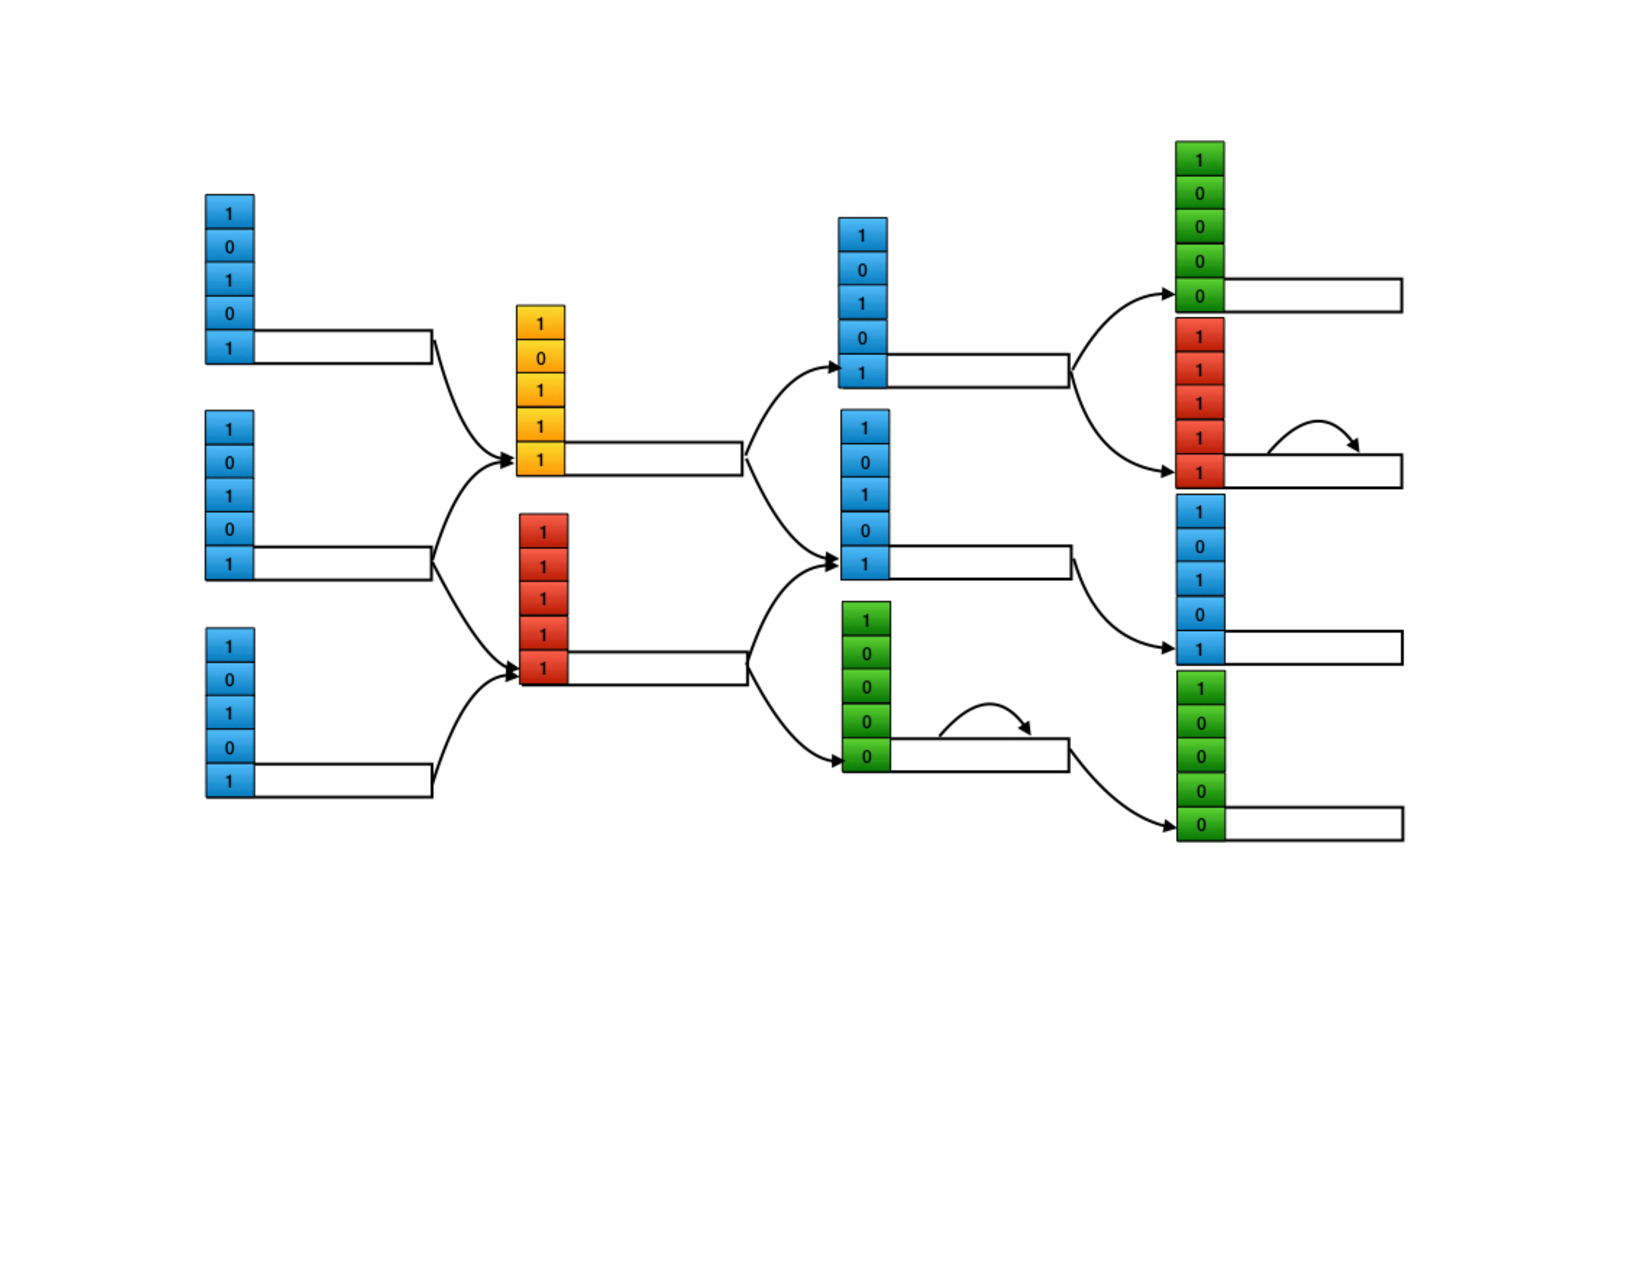
\includegraphics[width=0.7\columnwidth, trim={1in 2.5in 1.5in 1in},clip]{figs/mantis/cdbg}
        \caption{A colored de Bruijn graph.  Each rectangle node represents a \kmer.
        Each vector represents a color class (equal color classes have the same color).}
        \label{subfig-cdbg}
    \end{subfigure}%
    ~
    \begin{subfigure}[t]{0.49\textwidth}
        \captionsetup{width=0.7\columnwidth}
        \centering
        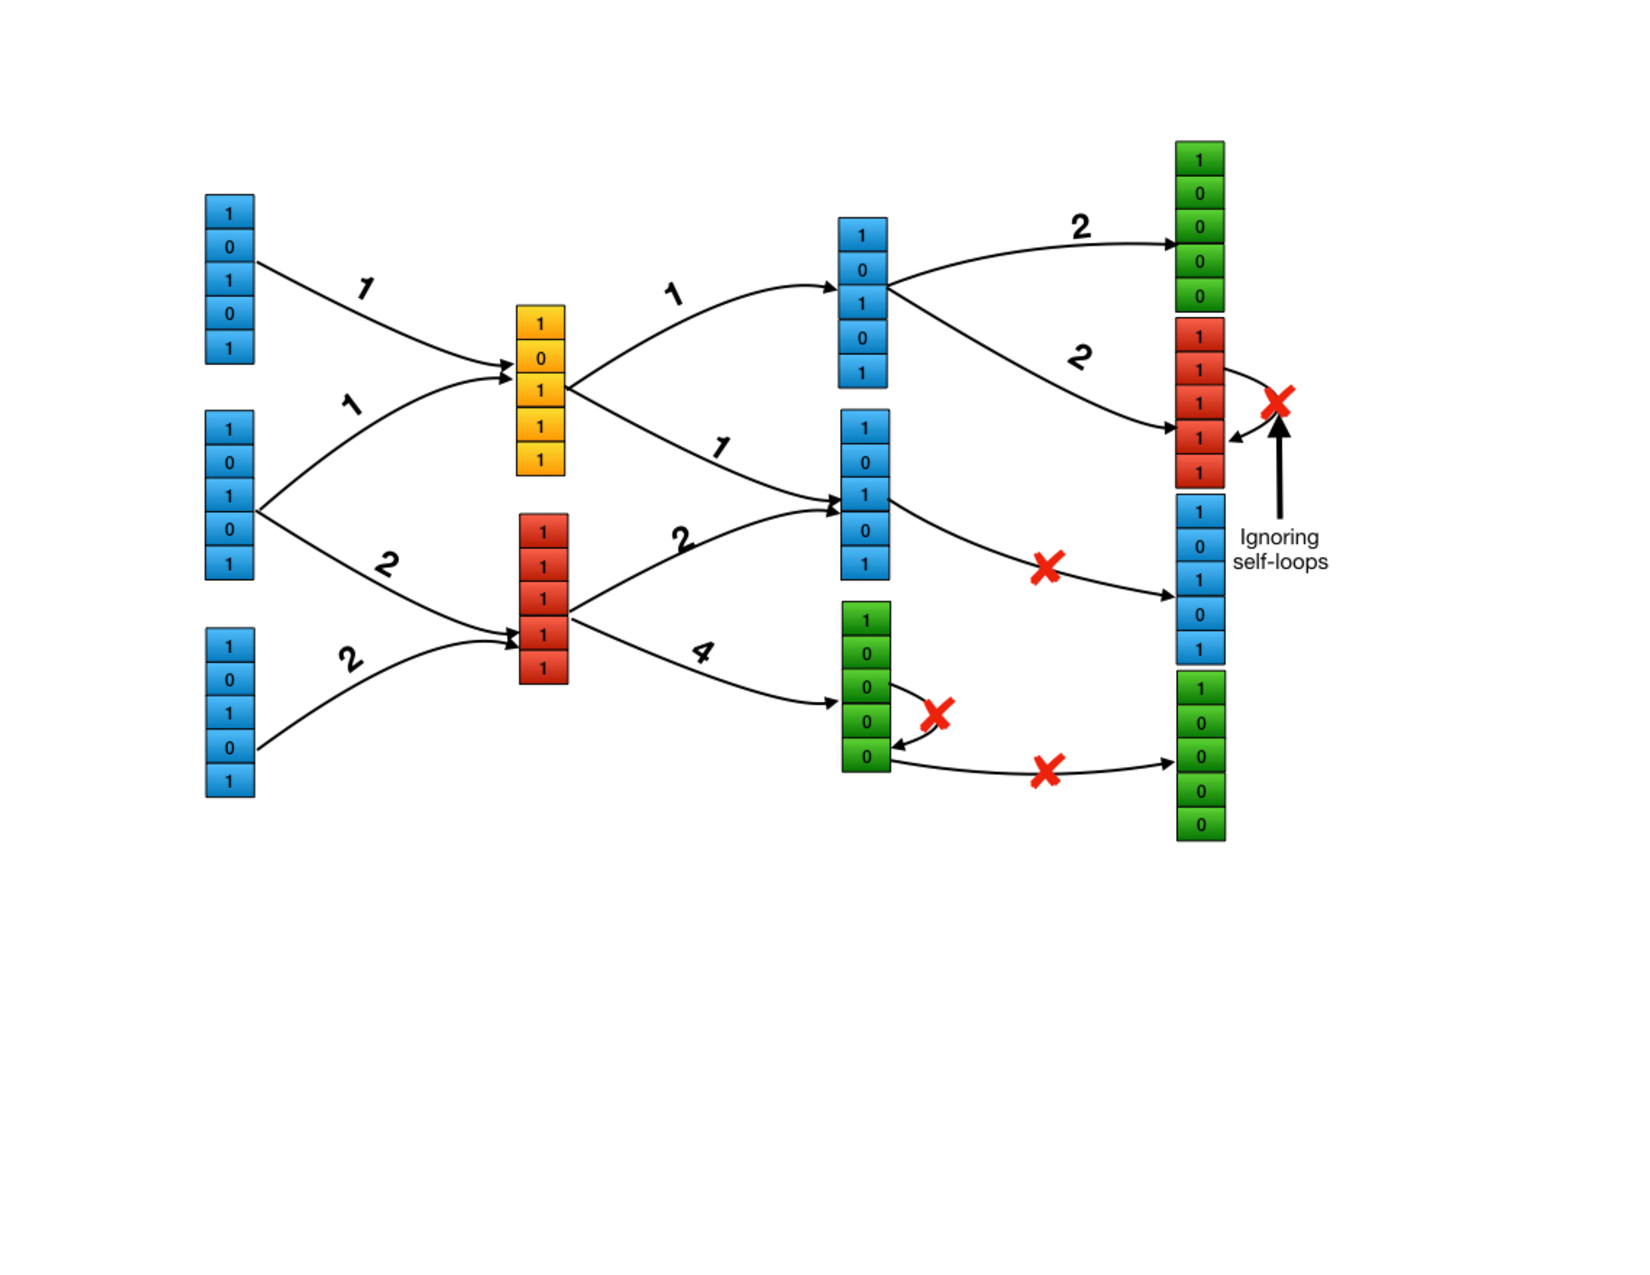
\includegraphics[width=0.7\columnwidth, trim={1in 2.5in 1.5in 1in},clip]{figs/mantis/cc}
        \caption{The \cc graph from the \cdbg. There is an edge between each pair of color classes
        that correspond to adjacent \kmers in \cdbg.
        Weights on the edges represent the Hamming distances of the \cc vectors.}
        \label{subfig-cc}
        \vspace{0.2in}
    \end{subfigure}
    ~

    \begin{subfigure}[t]{0.5\textwidth}
        \captionsetup{width=0.7\columnwidth}
        \centering
        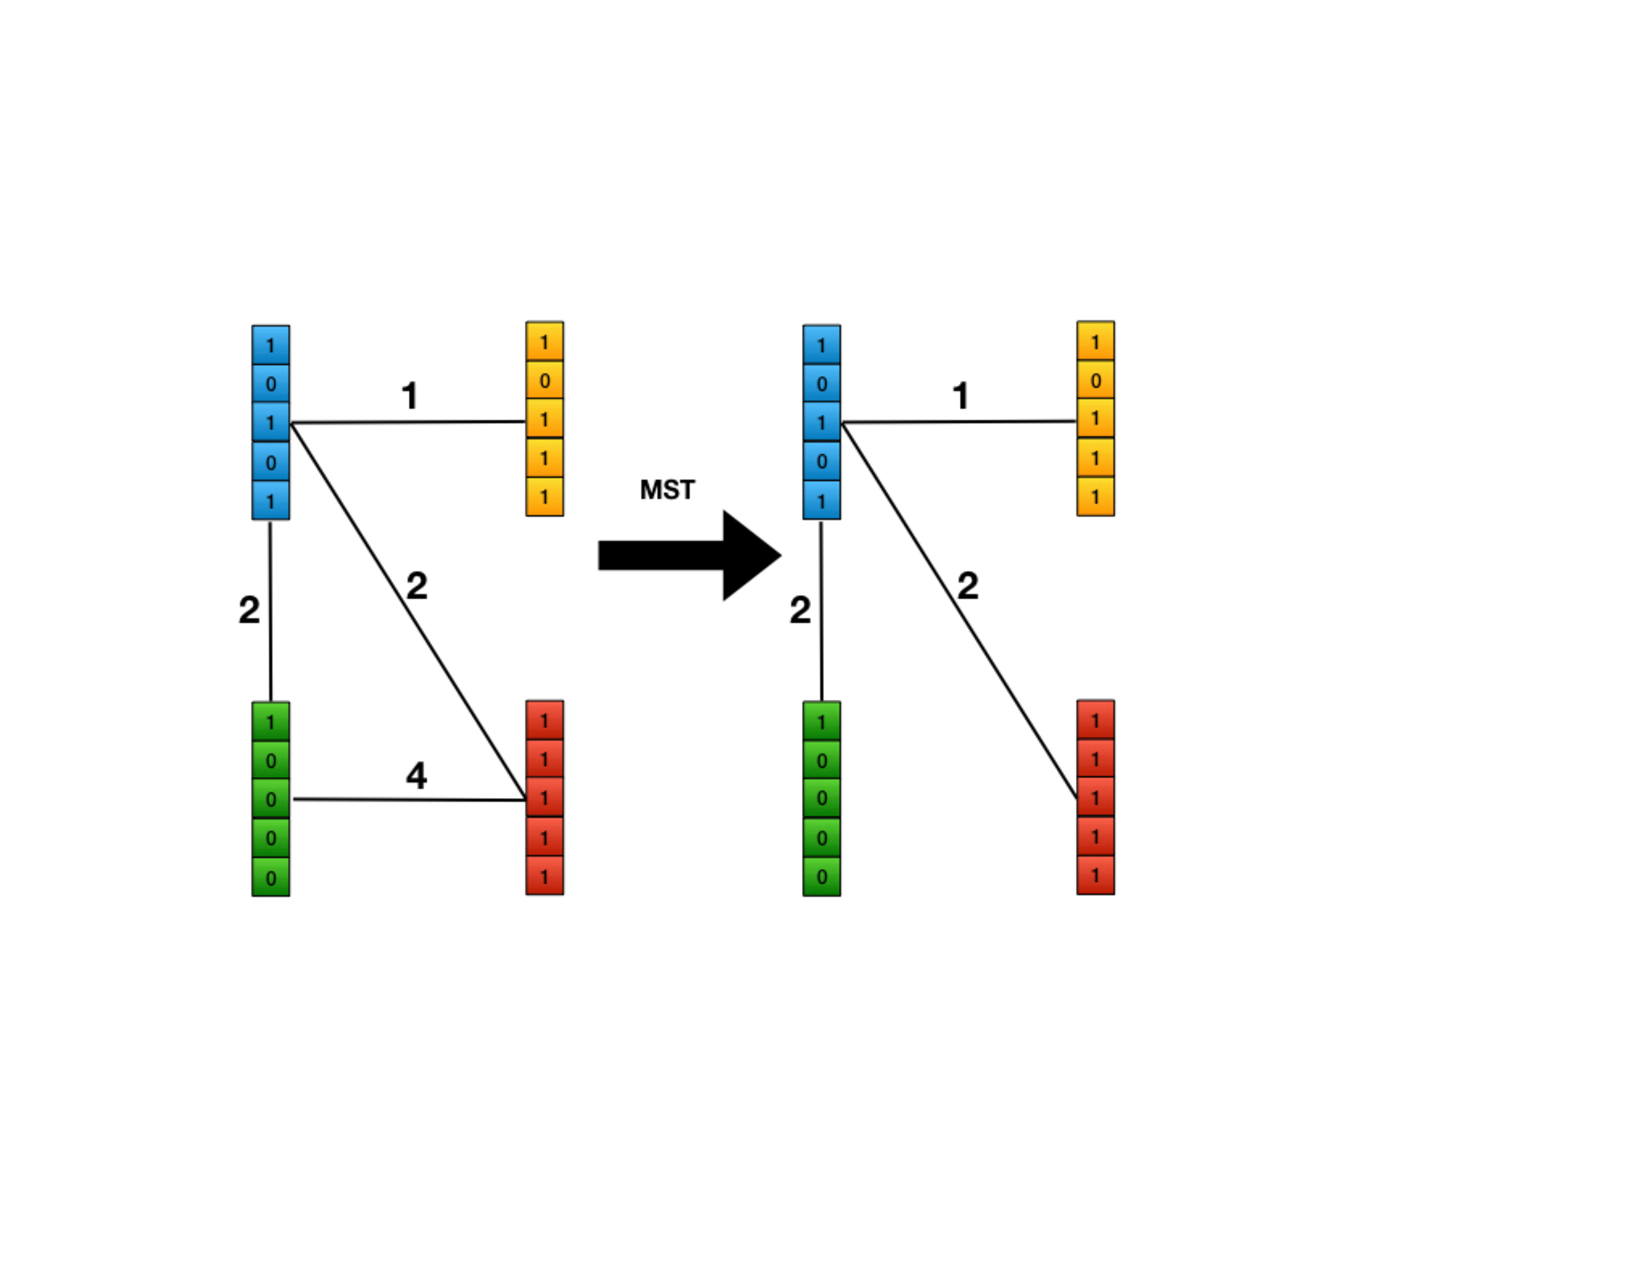
\includegraphics[width=0.7 \columnwidth, height=3.5cm, trim={1in 2in 2.5in 2in},clip]{figs/mantis/ourCg}
        \caption{The \cc graph we achieve from \ref{subfig-cc} by removing duplicate edges
        and its corresponding \mst.}
        \label{subfig-ourmst}
    \end{subfigure}%
    ~
    \begin{subfigure}[t]{0.5\textwidth}
        \captionsetup{width=0.7\columnwidth}
        \centering
        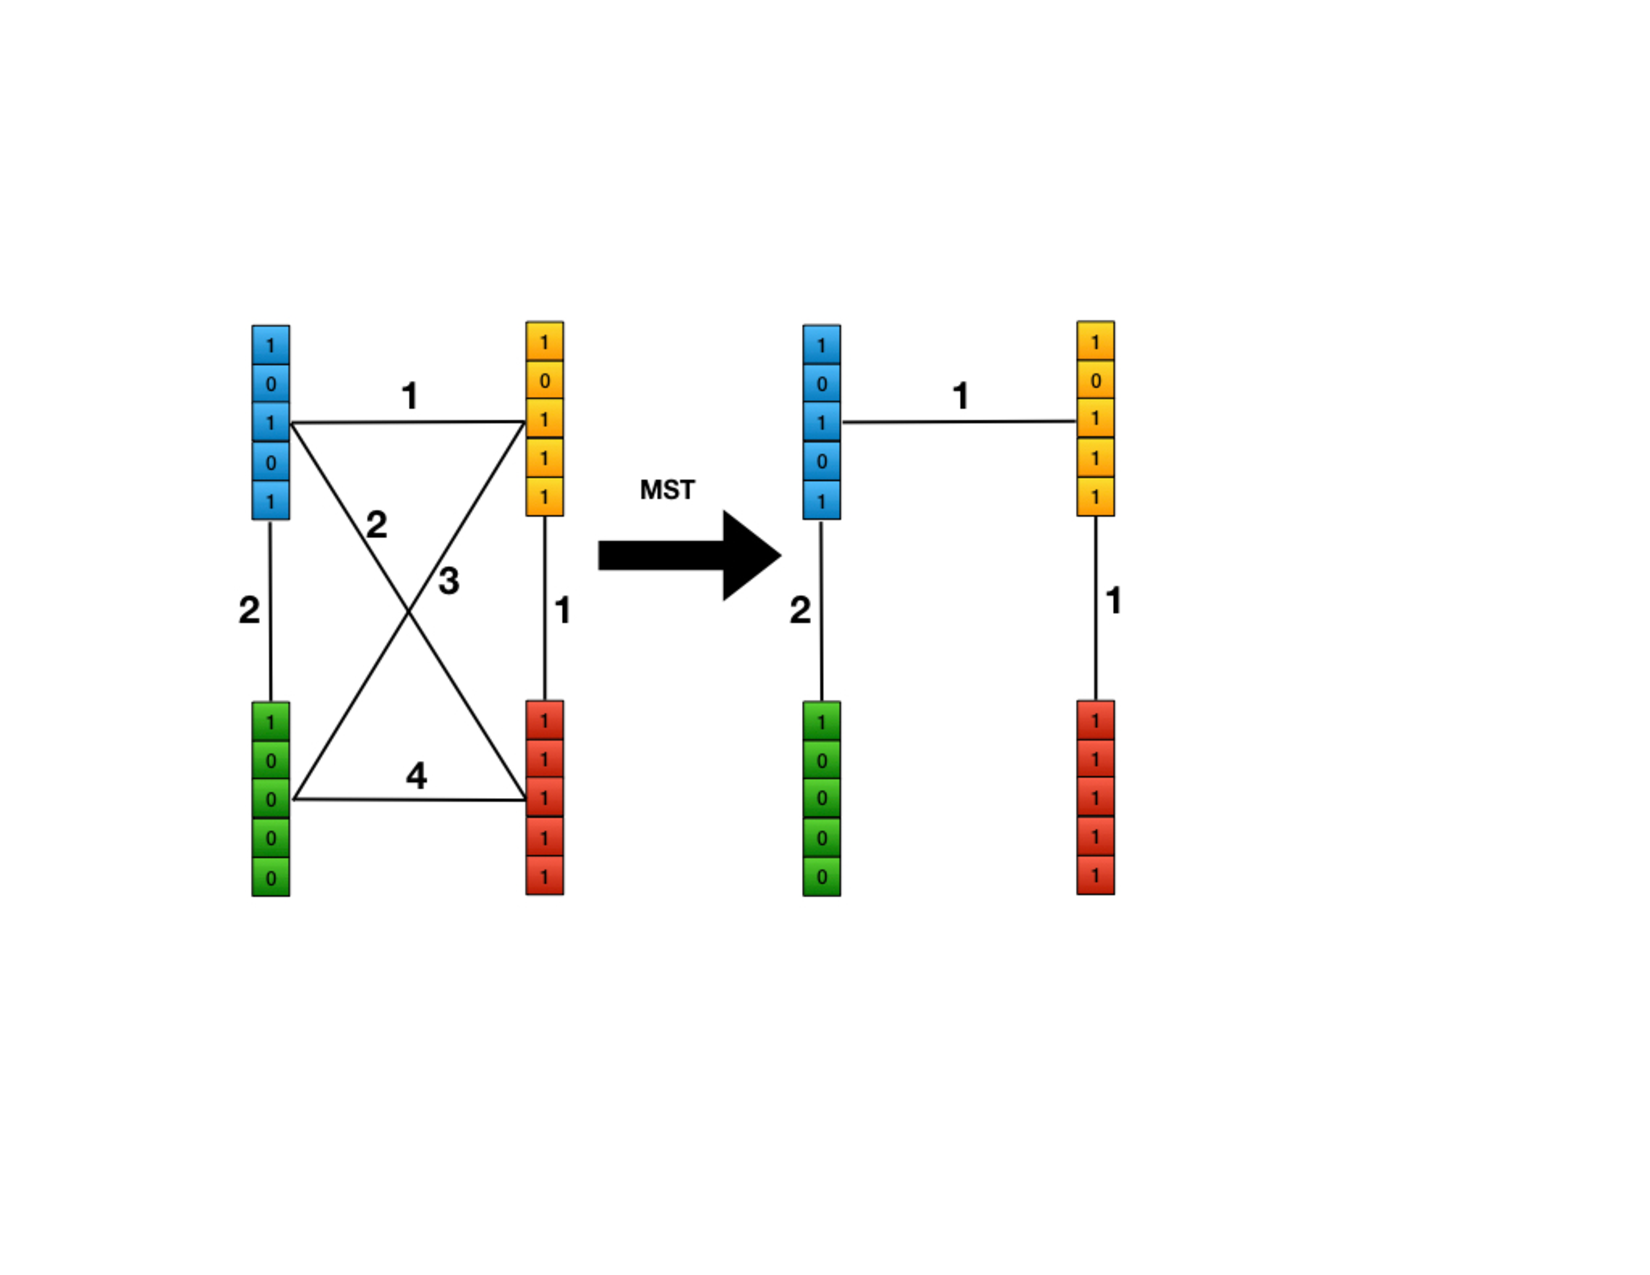
\includegraphics[width=0.7\columnwidth, height=3.5cm, trim={1in 2in 2.5in 2in},clip]{figs/mantis/optimalCg}
        \caption{The complete \cc graph
        and its derived \mst which has the minimum achievable total weight.}
        \label{subfig-optimalmst}
        \vspace{0.1in}
    \end{subfigure}
    \caption{Encoding \ccs by finding the \mst of the \cc graph, an undirected graph
    derived from \cdbg.
    The order of the process is \ref{subfig-cdbg}, \ref{subfig-cc},
    and \ref{subfig-ourmst}. The arrows in \ref{subfig-cdbg} and \ref{subfig-cc}
    show the direction of edges in the \dbg which is a directed graph. The optimal achievable
    \mst is shown in \ref{subfig-optimalmst} for comparison.
    Since we never observe the edge between any \kmers from \ccs green and yellow in \cdbg,
    we won't have the edge between \ccs green and yellow and therefore, our final \mst
    is not equal to the best \mst we can get from a complete \cc graph.
    }
    \label{fig:mstConstruction}
\end{figure*}


\subsection{Implementation of the MST data structure}

Assuming we have $|\calC|$ \ccs,
$|U|$ colors, and an \mst with total weight of $w$ over the \cc graph,
we store all the information required to retrieve the original \cbv for each \cc ID
based on the \mst structure into three data structures:
\begin{itemize}
    \item \textbf{Parent vector}: This vector contains $|\calC|$
    slots, each of size $\ceil{\log_2 {\calC}}$.  The value stored
    in index $i$ represents the parent \cc ID of the \cc with index
    $i$ in the \mst.
    \item \textbf{Delta vector}: This vector contains $w$ slots, each
    of size $\ceil{\log_2 {|U|}}$.  For each pair of parent and
    child in the parent vector, we compute a vector of the indices
    at which they differ.  The delta vector is the concatenation of
    these per-edge delta vectors, ordered by the ID of the source of
    the edge.  Note that the per-edge delta vectors will not all be
    of the same length, because some edges have larger weight than
    others.  Thus, we need an auxiliary data structure to record the
    boundaries between the per-edge deltas within the overall delta
    vector.
    %%   store the indices of the bits that are
    %% different between parent and child \cbvs. We call these different indices deltas of the two
    %% \cbvs. The order of the delta sets is the same as the order of the nodes in the \pbv.
    %    meaning that
    %     assuming $i \leq j$ be the indices of two child nodes in parent int-vector, the delta set
    %     for node $i$ and its parent comes before the delta set for node $j$ and its parent.
    \item \textbf{Boundary bit-vector}: This vector contains $w$ bits,
    where a set bit indicates the boundary between two delta sets
    within the delta vector.  To find the starting position, within
    the delta vector, of the per-edge delta list for the MST edge
    with source ID $i$, we perform \textit{select($i$)} on
    the boundary vector.  Select returns the position of the $i$th
    one in the boundary vector.
    %% For finding the deltas for a child at
    %% index $i$ in the parent vector and its parent, we use the
    %% succinct operation \textit{select} for index $i$ on the boundary
    %% bit-vector to find out the starting index of the delta set for
    %% $i$ in the delta int-vector.
\end{itemize}

\paragraph{Query of the \mst-based representation.} \Cref{fig:query} shows how queries proceed using this encoding.
We start with an empty accumulator bit vector and a color class ID $i$
for which we want to compute the corresponding color class.  We
perform a select query for $i$ and $i+1$ in the boundary bit-vector to get the
boundaries of $i$'s difference list in the delta vector.  We then
iterate over its difference list and flip the indicated bits in our
accumulator.  We then set $i\gets \textsc{parent}[i]$ and repeat
until $i$ becomes 0, which indicates that we have reached the root.
At this point, the accumulator will be equal to the bit vector for
color class $i$.

\begin{figure*}[t!]
    \centering
    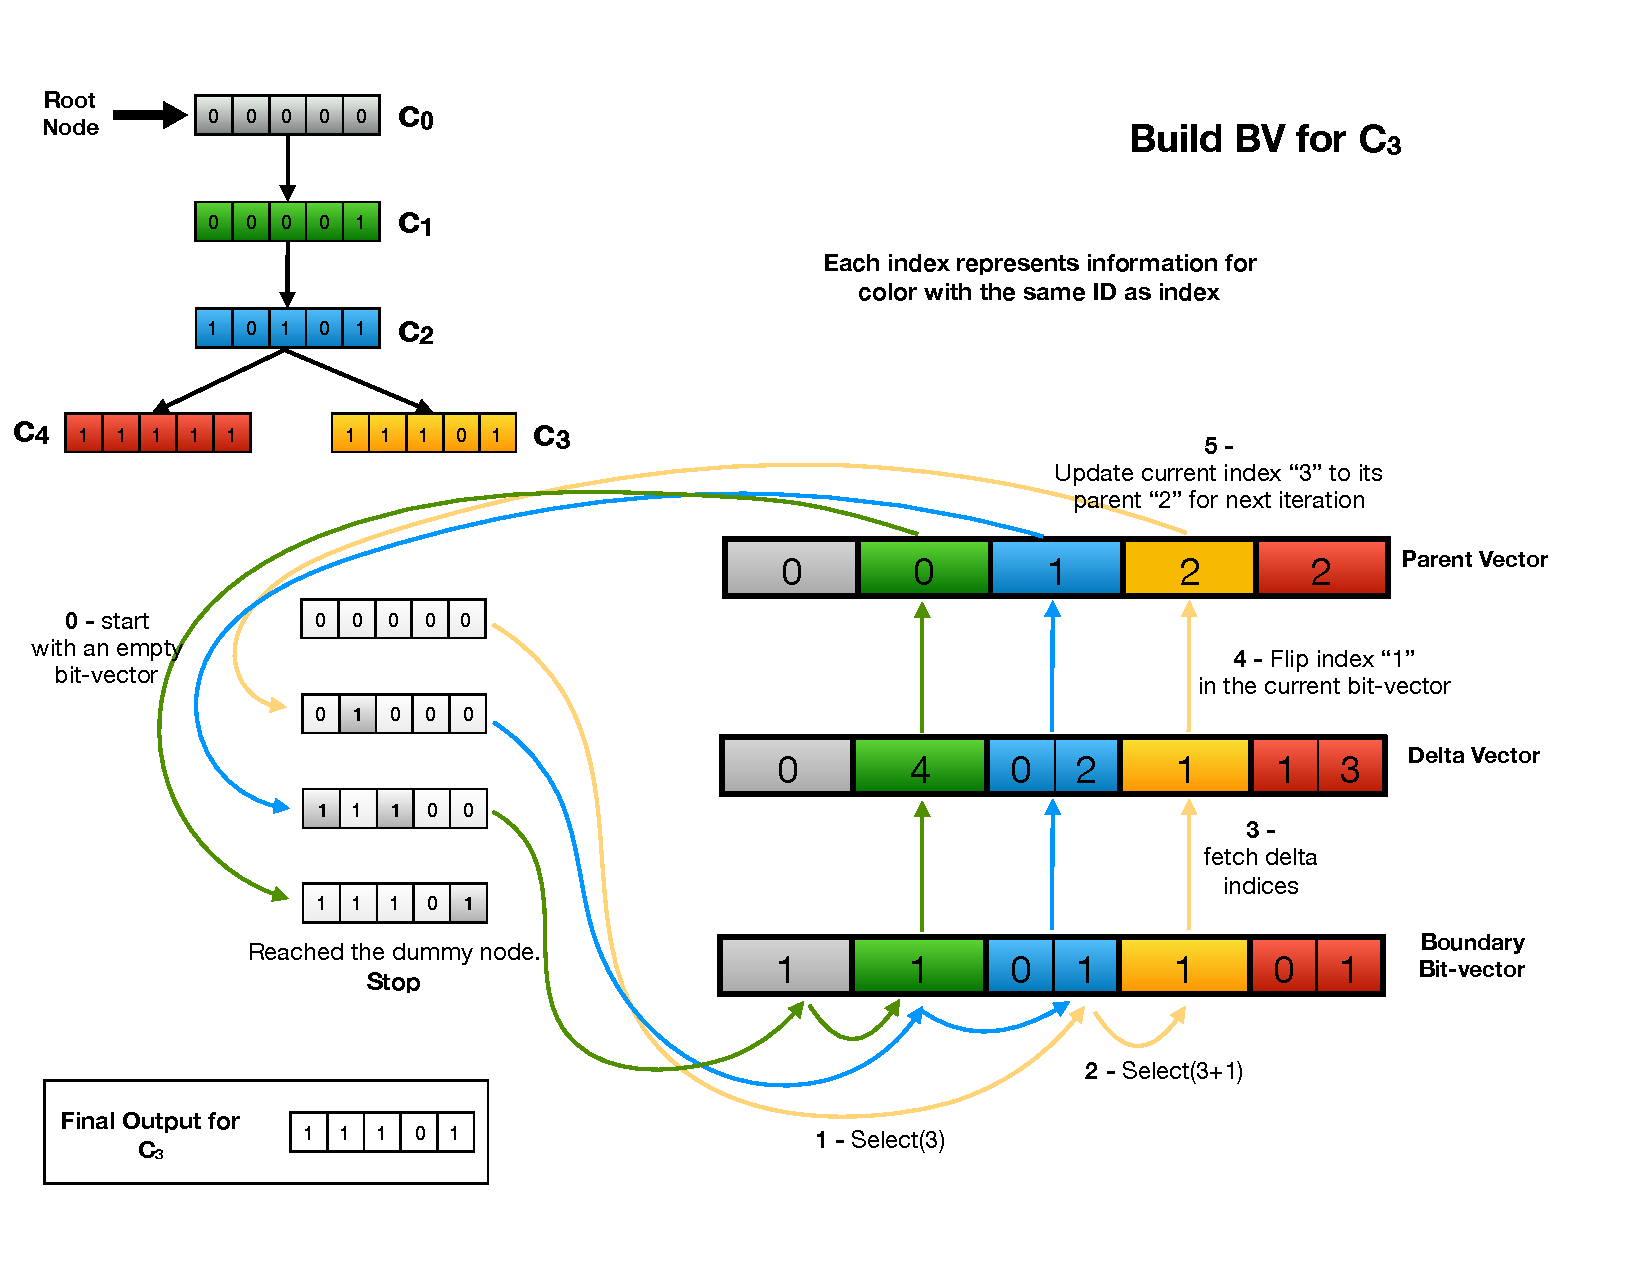
\includegraphics[width=0.65\columnwidth]{figs/mantis/figure2}
    \caption{The conceptual \mst (top-left), the data structure to
    store the color information in the format of an \mst (right).
    This figure also illustrates the steps required to build one of the color vectors ($C_3$) at the leaf
    of the tree. Note that the query process shown here does not depict the caching policy we apply in practice.}
    \label{fig:query}
    \vspace{-1.5em}
\end{figure*}


\subsection{Integration in Mantis}

Once constructed, our MST-based color class representation is a
drop-in replacement for the current color class representations used in
several existing tools, including Mantis~\cite{mantis} and
Rainbowfish~\cite{rainbowfish}.  Their existing color class
tables support a single operation---querying for a color class
by its ID---and our MST-based representation supports exactly
the same operation.

For this paper, we integrated our MST-based representation into
Mantis.  The same space savings can be achieved in
other tools, particularly Rainbowfish, which has
a similar color-class encoding as Mantis.

\ourparagraph{Construction.}
We construct our MST-based color-class representation as follows.
First, we run Mantis to build its default representation of the \cdbg.
We then build the color-class graph by walking the \dbg and adding all
the corresponding edges to the color-class graph.  The edge set is
typically much smaller than the \dbg (because many \dbg edges may map to
the same edge in the color-class graph), so this can be done in RAM.
Note that we do not compute the weights of the edges during this pass,
because that would require having all of the large color-class bit vectors
in memory in order to compute their Hamming distance.
%walk the \cdbg to determine which distinct colors are adjacent
%in the underlying \dbg.  This provides us with an edge set for our
%color graph.

In the second pass, we traverse the edge set and compute the weight of
each edge.  To minimize RAM usage during this phase, we sort
the edges and iterate over them in a ``blocked'' fashion.
Specifically, Mantis stores the color class bit vectors on-disk
sequentially by ID, grouped into blocks of roughly 6GBs each.  We sort
the edges lexicographically by their source and destination block. We then load
all pairs of blocks and compute the weights of all the edges between the two
blocks currently in memory. At all times, we need only two blocks of color class
vectors in memory. Given the weighted graph, we compute the \mst and make one
final pass to determine the relevant delta lists and encode our final \mst
structure.

\ourparagraph{Parallelization.}  We note that, after having
constructed the \prevsys representation, most phases of the MST
construction algorithm are trivially parallelized.  MST construction
decomposes into three phases: (1) color-class graph construction, (2)
MST computation, and (3) color-class representation generation.
We parallelize graph construction and color-class representation
generation. The MST computation itself is not parallelized.

We parallelized the determination of edges in the color-class graph by
assigning each thread a range of the \kmer-to-color-class-ID
map. Each thread explores the neighbors of the \kmers that appear in
its assigned range, and any redundant edges are deduplicated when all
threads are finished.  Similarly, we parallelized the computation of
edge weights and the extraction of the delta vectors that correspond
to each edge in the MST. Given the list of edges sorted
lexicographically by their endpoints (determined during the first
phase), it is straightforward to partition the work for processing
batches of edges across many threads. It is possible, of course, that
the batches will display different workloads and that some threads
will complete their assigned work before others.  We have not yet made
any attempt to optimize the parallel construction of the MST in this
regard, though many such optimizations are likely possible.

\ourparagraph{Accelerating queries with caching.}
The encoded \mst is not a balanced tree, so decoding a \cbv might require
walking a long path to the root, which negatively impacts the query time.
Attempting to explicitly minimize the depth or diameter of the MST is, as
discussed in~\Cref{sec:intro}, not generally approximable within a constant
factor. However, considering the fact that the frequency distribution of
the \ccs is very skewed, some of the \ccs are more popular or have more children
and, therefore, are in the path of many more nodes. We take advantage of these
data characteristics by caching the most recent queried \cbvs. Every time we
walk up the tree, if the \cbv for a node is already in the cache, our query
algorithm stops at that point and applies all the deltas to this \bv instead of
the zero \bv of the root. This caching approach significantly improves the query
time, resulting in the final query time required to decode a \cc being
marginally faster than direct RRR access.

The cache policy is designed with the tree structure of our
color-class representation in mind.  Specifically, we want to cache
nodes near the leaves, but not so close to the leaves that we end up
caching essentially the entire tree.  Also, we don't want to cache
infrequently queried nodes.  Thus we use the following caching policy:
all queried nodes are cached.  Furthermore, we cache interior nodes
visited during a query as follows.  If a query visits a node that
has been visited by more than 10 other queries and is more than
10 hops away from the currently queried item, then we add that node
to the cache.  If a query visits more than one such node, we add
the first one encountered.

In our experiments, we used a cache of 10,000 nodes and managed the
cache using a FIFO policy.

\subsection{Comparison with brute-force and approximate-nearest-neighbor-based approaches}

Our MST-based color-class representation uses the \dbg as a hint as to
which color classes are likely to be similar.  This leads to the
natural question: how good are the hints provided by the \dbg?

One could imagine alternatively constructing the MST on the complete
color-class graph.  This would yield the absolutely lowest-weight
spanning tree on the color classes.  Unfortunately, no MST algorithm
runs in less than $\Omega(|E|)$ time, so this would make our
construction time quadratic in the number of color classes.  The
number of color classes in our experiments range from $10^{6}$ to
$10^9$, so the number of edges in the complete color-class graph would
be on the order of $10^{12}$ to $10^{18}$, or possibly even more,
making this algorithm impractical for the largest data sets considered
in this paper.

Alternatively, we could try to use an approximate nearest-neighbor
algorithm to find pairs of color classes with small Hamming distance.
As an experiment, we implemented an approximate nearest neighbor
algorithm that bucketed color classes by their projection into
a smaller-dimensional subspace.  Nearest-neighbor queries were
computed by searching within the queried item's bucket.
Results were disappointing.  Even on small data sets, the average
distance between the queried item and the returned neighbor
was several times larger than the average distance found using
the neighbors suggested by the \dbg.  Thus, we did not pursue
this direction further.

%%%%%%%%%%%%%%%%%%%%%%%%%%%%%%%%%%%%%%%%%%%%%%%%%%%%%%%%%%%%
%%
%% Results section
%%
%%%%%%%%%%%%%%%%%%%%%%%%%%%%%%%%%%%%%%%%%%%%%%%%%%%%%%%%%%%%
\section{Evaluation}
\label{sec:mantis_eval}

In this section we evaluate our MST-based representation of the color
information in the \cdbg.  All our experiments use Mantis with
our integrated MST-based color-class representation.


\ourparagraph{Evaluation Metrics}
We evaluate our MST-based representation on the following parameters:
\begin{itemize}
    \item \textbf{Scalability.} How does our MST-based color-class representation
    scale in terms of space with increasing number of input samples, and how does
    it compare to the existing representations of \prevsys?

    \item \textbf{Construction time.} How long does it take --- in addition to
    the original construction time for building \cdbg --- to build
    our MST-based color-class representation?

    \item \textbf{Query performance.} How long does it takes to query the \cdbg
    using our MST-based color-class representation?
\end{itemize}
\subsection{Experimental procedure}

\label{experimental-proc}

\ourparagraph{System Specifications}

Mantis takes as input a collection of \defn{squeakr} files~\cite{PandeyBeJo17}.
Squeakr is a \kmer counter that takes as input a collection of fastq
files and produces as output, a single file with a compact hash table
mapping each \kmer to the number of times it occurs in the input
files.  As is standard in evaluations of large-scale sequence search indexes,
we do not benchmark the time required to construct these filters.

The data input to the construction process
was stored on 4-disk mirrors (8 disks
total).  Each is a Seagate 7200rpm 8TB disk (ST8000VN0022). They were formatted
using ZFS and exported via NFS over a 10Gb link.
We used different systems to run and evaluate time, memory,
and disk requirements for the two steps of preprocessing and
index building as was done by~\citet{mantis}.

For index building and query benchmarks, we ran all the experiments on
the same system used in \prevsys~\citep{mantis}, an
Intel(R) Xeon(R) CPU (E5-2699 v4 @2.20GHz with 44 cores and 56MB L3 cache) with
512GB RAM and a 4TB TOSHIBA MG03ACA4 ATA HDD running Ubuntu 16.10 (Linux kernel
4.8.0-59-generic).  Constructing the main index was done using a single thread,
and the MST construction was performed using $16$ threads.  Query benchmarks
were also performed using a single thread.

% Explaining the 10,000 experiments
\ourparagraph{Data to evaluate scalability and comparison to \prevsys}

We integrated and evaluated our MST-based color-class representation
within Mantis, so we briefly review Mantis here. Mantis builds an index on a
collection of unassembled raw sequencing data sets. Each data set is called a
\defn{sample}. The Mantis index enables fast queries of the form, ``Which
samples contain this \kmer,'' and ``Which samples are likely to contain this
string of bases?'' Mantis takes as input one \defn{squeakr} file per
sample~\cite{PandeyBeJo17}. A squeakr file is a compact hash table mapping each
\kmer to the number of times it occurs within that sample. \squeakr also has the
ability to serialize a hash that simply represents the set of \kmers present at
or above some user-provided threshold; we refer to these as filtered \squeakr
files. Using the filtered \squeakr files vastly reduces the required
intermediate storage space, and also decreases the construction time required
for Mantis considerably. For example, for the breast, blood, and brain dataset
($2586$ samples), the unfiltered \squeakr files required $\sim2.5$TB of space
while the filtered files require only $\sim108$GB. To save intermediate storage
space and speed index construction, we built our Mantis representation from
these filtered \squeakr files.


Given the input files, Mantis constructs an index consisting of two
files: a map from \kmer to color-class ID, and a map from color-class
ID to the bit vector encoding that color class.  The first map is
stored as a \defn{counting quotient filter} (CQF), which is the same
compact hash table used by Squeakr.  The color-class map is an
RRR-compressed bit vector.

Recall that our construction process is implemented as a
post-processing step on the standard Mantis color-class
representation.  For construction times, we report only this
post-processing step.  This is because our MST-based color-class
representation is a generic tool that can be applied to many \cdbg
representations other than Mantis, so we want to isolate the time
spent on MST construction.

To test the scalability of our new \cc representation, we used a
randomly-selected set of $10,000$ paired-end, human, bulk RNA-seq short-read
experiments downloaded from European Nucleotide Archive(ENA)~\citep{nih-sra} in
gzipped FASTQ format. Additionally, we have built the proposed index for
$2,586$ sequencing samples from human blood, brain, and breast tissues (\bbb)
originally used by~\cite{Solomon2016Fast} and also used in the subsequent
work~\citep{Solomon2017Improved,Sun2017Allsome,seqothello}, including
\prevsys~\citep{mantis}, as a point of comparison with these representations.
The set of $10,000$ experiments does not overlap with the \bbb samples.
The full list of $10,000$ experimental identifiers can be obtained from
\url{https://github.com/COMBINE-lab/color-mst/blob/master/input_lists/nobbb10k_shuffled.lst}.
%\url{https://github.com/COMBINE-lab/color-mst/blob/master/input_lists/shuffled_10k_paired}.
The total size of all these experiments (gzipped) is $25.23$TB.
%new result: 27745362006992%%%old result: 27550806707164%

% Cutoffs
In order to eliminate spurious \kmers that
occur with insignificant abundance within a sample, the squeakr files
are filtered to remove low-abundance \kmers.
We adopted the same cutoff policy originally proposed by~\citet{Solomon2016Fast},
by discarding \kmers that occur less than some threshold number of time.  The
thresholds are determined according to the size (in bytes) of the gzipped
sample, and the thresholds are given in \Cref{tab:cutoffs}.  We adopt a value of
$k=23$ for all experiments.
\begin{table}[t]
    \centering
    \begin{tabular}{r@{\hskip 0.5in}r@{\hskip 0.5in}r@{\hskip 0.5in}c}
        \hline
        Min size & Max size    & Cutoff & \begin{tabular}{c}\# of experiments \\ with specified threshold\end{tabular}\\
        \hline
        \hline
        0        & $\leq 300$MB   & 1  & 2,784\\
        $>300$MB & $\leq 500$MB   & 3  & 798\\
        $>500$MB & $\leq 1$GB     & 10 & 1,258\\
        $>1$GB   & $\leq 3$GB     & 20 & 2,296\\
        $>3$GB   & $\infty$       & 50 & 2,864\\
        \hline
    \end{tabular}
    \caption{\label{tab:cutoffs}Minimum number of times a \kmer must
    appear in an experiment in order to be counted as abundantly
    represented in that experiment (taken from the SBT paper). Note,
    the \kmers with count of ``cutoff'' \emph{are} included at each
    threshold.}
    \vspace{-2.5em}
\end{table}

\subsection{Evaluation results}

\ourparagraph{Scalability of the new \cc representation}
\Cref{fig:scaling} and \Cref{tab:growthrate} show how the size of our
MST-based color-class representation scales as we increase the number
of samples indexed by Mantis.  For comparison, we also give the size
of Mantis' RRR-compression-based color-class representation.
\Cref{fig:scaling} also plots the size of the CQF that Mantis uses to
map \kmers to color class IDs. We can draw several conclusions from this data:
\begin{itemize}
    \item {The MST-based representation is an order-of-magnitude
    smaller than the RRR-based representation.}
    \item {The gap between the RRR-based representation and the
    MST-based representation grows as we increase the number of input
    samples.}  This suggests that the MST-based representation
    grows asymptotically slower than the RRR-based representation.
    \item {The MST-based color-class representation is, for large
    numbers of samples, about 5$\times$ smaller than the CQF.}  This
    means that representing the color classes is no longer the scaling
    bottleneck.
\end{itemize}

\begin{figure*}[t!]
    %    \captionsetup[subfigure]{justification=centering}
    \centering
    \begin{subfigure}[t]{3in}
        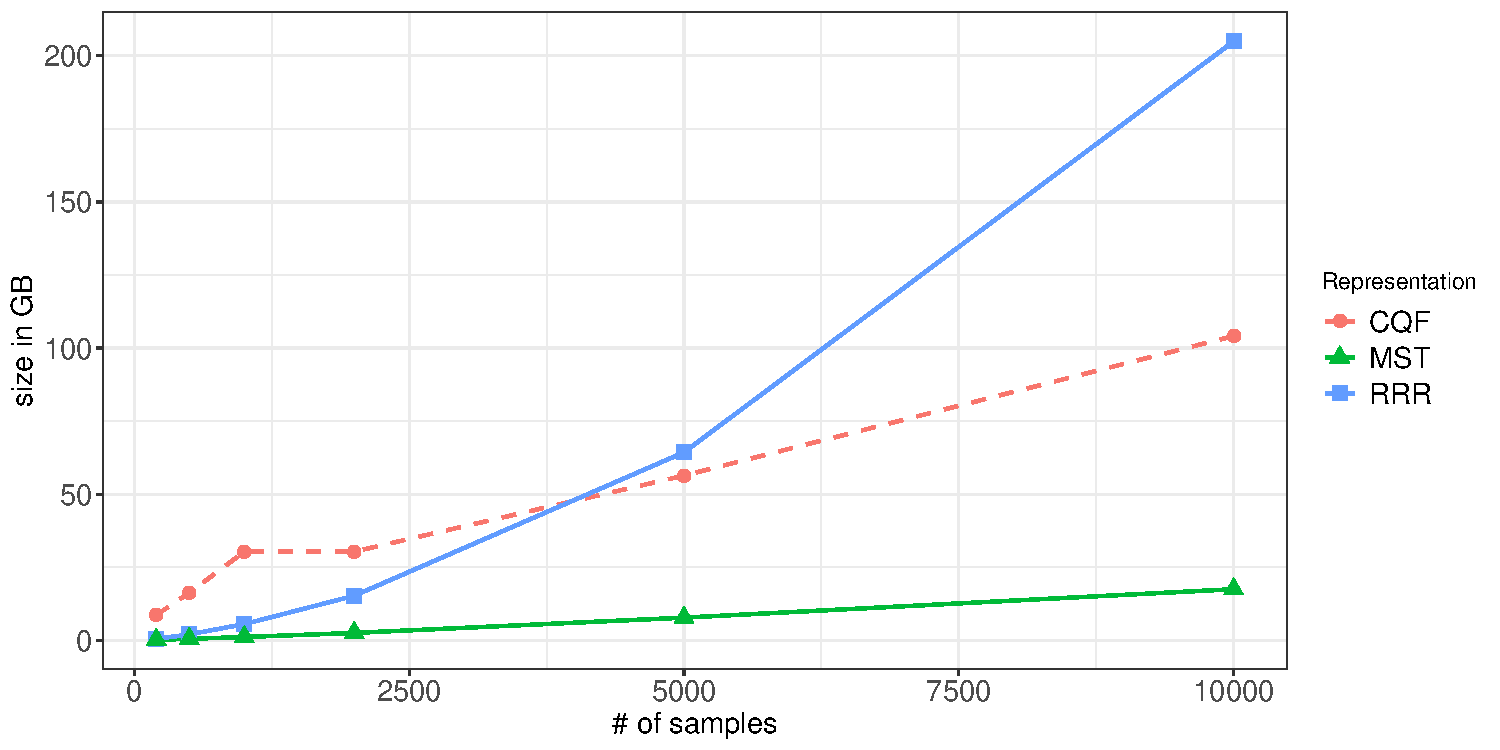
\includegraphics[width=3in]{figs/mantis/scaling_r2}
        \caption{Sizes of the RRR and \mst-based \cc representations with
        respect to the number of samples indexed from the human bulk RNA-seq data set.
        The \cqf component is the Mantis representation of the \dbg.}
        \label{fig:scaling}
    \end{subfigure}
    ~~~~~~~~~~~
    \begin{subfigure}[t]{3in}
        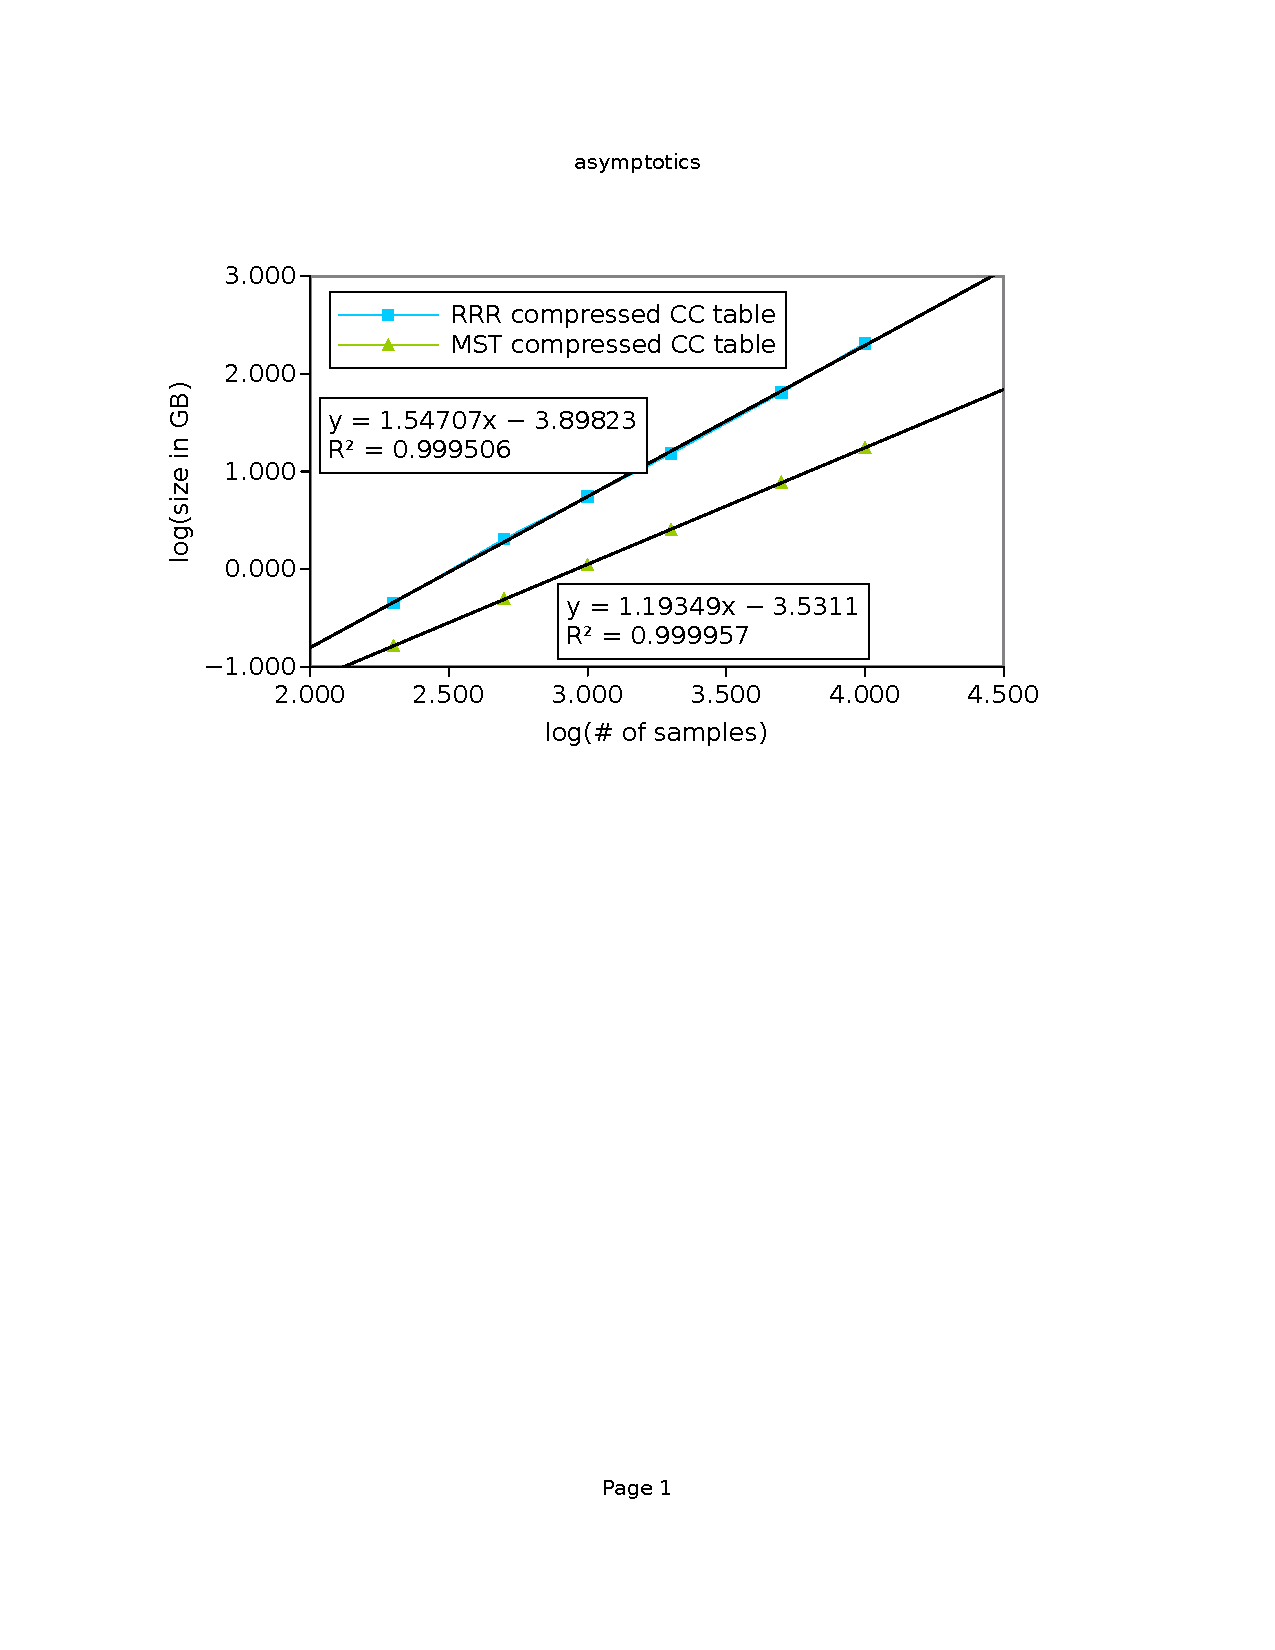
\includegraphics[width=3in,clip, trim = 1.1in 6in 1.5in 1.75in]{figs/mantis/asymptotics__asymptotics}
        \caption{Empirical asymptotic analysis of the growth rates of the
        sizes of RRR-based \cc representation and the MST-based
        \cc representation.  The RRR-based representation grows
        at a rate of $\approx \Theta(n^{1.5})$, where $n$ is the number of
        samples.  The MST-based representation grows at a rate of
        $\approx\Theta(n^{1.2})$.}
        \label{fig:asymptotics}
        \vspace{.1in}
    \end{subfigure}
    \caption{Size of the MST-based color-class representation vs.
    the RRR-based color-class representation.}
\end{figure*}

\Cref{tab:growthrate} also shows the scaling rate of all elements of
the \mst representation, in addition to the ratio of \mst over the
\cbv.  As expected, the list of deltas dominate the \mst
representation both in terms of total size and in terms of
growth. \Cref{tab:growthrate} also shows the average edge weight of
the edges in the \mst.  The edge weight grows approximately
proportional to $\Theta(\log(\text{\# of samples}))$ (i.e., every time
we double the number of samples, the average edge weight increases by
almost exactly 1). This suggests that our \dbg-based algorithm
is able to find pairs of similar color classes. The time column shows the time
required to build the \mst representation (which is in addition to the \prevsys
construction time required to produce the input to the \mst compression
algorithm).

To better understand the scaling of the different components of a
\cdbg representation, we plot the sizes of the RRR-based color-class
representations and MST-based representations on a log-log scale in
\Cref{fig:asymptotics}. Based on the data, the RRR-based
representation appears to grow in size at a rate of roughly
$\Theta(n^{1.5})$, whereas the new MST-based representation grows
roughly at a rate of $\Theta(n^{1.2})$. This explains why the
RRR-based representation grows to dwarf the CQF (which grows roughly
linearly) and become the bottleneck to scaling to larger data sets,
whereas the MST-based representation does not. With the MST-based
representation, the CQF itself is now the bottleneck.

Finally, the last two rows in \Cref{tab:growthrate} show the size of the RRR- and MST-based
color-class representations for the human blood, brain, breast (\bbb) and \textit{E. coli} data sets respectively.
\bbb is the data set used in \sbt and
its subsequent tools~\citep{Solomon2017Improved,Sun2017Allsome,seqothello},
as well as in \prevsys~\citep{mantis}
and \textit{E. coli} is the data set analyzed in the Rainbowfish paper.
This dataset, which has been obtained from
GenBank~\cite{o2015reference}, consists of $5,598$ distinct \emph{E. coli}
strains. Since the strain assemblies are all from the same species,
\emph{E. coli}, each strain shares a large portion of its sequence with the others.
We specifically chose this dataset since \rainbowfish has already
demonstrated a large improvement in size for it compared to
Vari~\citep{MuggliBoNo17}.

As the table shows, our MST-based
color-class representation is able to effectively compress genomic
color data in addition to RNA-seq color data.

\begin{table}[t]
    \centering
    \resizebox{\columnwidth}{!}{%
    \begin{tabular}{c|c@{\hskip 0.05in}c@{\hskip 0.05in}c@{\hskip 0.05in}c
    @{\hskip 0.05in}c@{\hskip 0.05in}c@{\hskip 0.05in}c@{\hskip 0.05in}c
    @{\hskip 0.15in}c@{\hskip 0.15in}c}
        \hline
        & & & \multicolumn{4}{c}{MST} \\ \cline{4-9}
        \multicolumn{1}{p{1.5cm}|}{\centering Dataset}
        & \multicolumn{1}{p{1.5cm}}{\centering \# samples}
        & \multicolumn{1}{p{1.5cm}}{\centering RRR matrix}
        & \multicolumn{1}{p{1.5cm}}{\centering Total \\ space}
        & \multicolumn{1}{p{1.5cm}}{\centering Parent \\ vector}
        & \multicolumn{1}{p{1.5cm}}{\centering Delta \\ vector}
        & \multicolumn{1}{p{1.5cm}}{\centering Boundary \\ bit-vector}
        %     & \multicolumn{1}{p{1.5cm}}{\centering Build \\ memory \\ (GB)}
        & \multicolumn{1}{p{1.5cm}}{\centering Build \\ time \\ (hh:mm:ss)}
        & \multicolumn{1}{p{1.5cm}}{\centering Expected \\ edge weight}
        & \multicolumn{1}{p{1.5cm}}{\centering $\frac{\text{size}(\mst)}{\text{size}(\text{RRR})}$}
        \\
        %& $\frac{weight(\mst)}{count(edges)}$ \\
        \hline
        \hline
        \multirow{6}{*}{\begin{tabular}{c}\textit{H. sapiens} \\ RNA-seq \\ samples\end{tabular}}
        & 200    & 0.42 & 0.15 & 0.08 & 0.06 & 0.01 & 0:05:42 & 2.42 & 0.37   \\ % mst/cbv: 68050395/28923216
        & 500    & 1.89 & 0.46	& 0.2 & 0.24	& 0.03	& 0:12:15 & 3.42 & 0.24  \\ % mst/cbv: 213655826/62036089
        & 1,000  & 5.14 & 1.03 & 0.37 & 0.6 & 0.06 & 0:25:03 & 4.39 & 0.2   \\ % mst/cbv: 492089063/110586891
        & 2,000  & 14.2 & 2.35 & 0.71 & 1.5 & 0.14 & 0:51:58 & 5.38 & 0.17  \\ % mst/cbv: 1092711068/198418790
        & 5,000  & 59.89 & 7.21 & 1.72 & 5.1 & 0.39 & 3:52:34 & 6.61 & 0.12   \\ % mst/cbv: 3120503401/457178572
        & 10,000 & 190.89 & 16.28 & 3.37 & 12.06 & 0.86 & 10:17:42 & 7.68 & 0.085  \\ % mst/cbv: 6974169057/893128926
        \hline
        \begin{tabular}{c} Blood, Brain,\\Breast (\bbb) \end{tabular} & 2586 & 15.8 & 2.66 & 0.63 & 1.88 & 0.16 & 00:57:43 & 6.98 & 0.17 \\
        \hline
        \begin{tabular}{c}\textit{E. coli} strain \\ reference genomes\end{tabular} & 5,598 & 2.06 & 0.83 & 0.02 & 0.76 & 0.06 & 00:03:15 & 7.8 & 0.4 \\ % mst/cbv: 6974169057/893128926
        \hline
    \end{tabular}
    }
    \vspace{0.1in}
    \caption{Space required for RRR and \mst-based \cc encodings over different numbers of samples (sizes in GB)
    and time and memory required to build \mst. Central columns break down the size of individual \mst components.}
    \label{tab:growthrate}
    \vspace{-1em}
\end{table}

\begin{table}[t]
    \centering
    %\resizebox{\columnwidth}{!}{%
    \begin{tabular}{c|c@{\hskip 0.05in}c@{\hskip 0.05in}c}
        \hline
        \multicolumn{1}{p{1.5cm}|}{\centering Dataset}
        & \multicolumn{1}{p{1.5cm}}{\centering \# samples}
        & \multicolumn{1}{p{3cm}}{\centering Mantis Build memory (GB)}
        & \multicolumn{1}{p{2cm}}{\centering MST Build memory (GB)}
        \\
        \hline
        \hline
        \multirow{6}{*}{\begin{tabular}{c}\textit{H. sapiens} \\ RNA-seq \\ samples\end{tabular}}
        & 200    & 5 & 8 \\
        & 500    & 10 & 16 \\
        & 1,000  & 18 & 29 \\
        & 2,000  & 25 & 29 \\
        & 5,000  & 58 & 59 \\
        & 10,000 & 111 & 111 \\
        \hline
        \begin{tabular}{c} Blood, Brain,\\Breast (\bbb) \end{tabular} & 2586 & 28 & 29 \\
        \hline
        %\begin{tabular}{c}\textit{E. coli} strain \\ reference genomes\end{tabular} & 5,598 & 4?? & 6 \\
        %\hline
    \end{tabular}
    \vspace{0.1in}
    \caption{The memory required for \prevsys build and \mst compression phases on
    human RNA-seq data. The overall memory required to construct the full index
    is the max of the two columns which, for these datasets, is always the \mst memory.}
    \label{tab:memory}
    \vspace{-1em}
\end{table}


\ourparagraph{Index Building Evaluation}
% Preprocessing
%Both tools \system and \seqothello have a preprocessing part before building the final index.
The ``Build time'' column in \Cref{tab:growthrate}
%\Cref{fig:mst-building-benchmark}
shows the time required to build our
MST-based color-class representation from Mantis' RRR-based
representation. All builds used 16 threads.
\Cref{tab:paraBenchmarks} shows how the \mst construction time for a $1000$
sample dataset scales as a function of the number of build threads. The memory
consumption is not affected by number of threads and remains fixed for all
trials.
The memory usage for both the main \prevsys build and the \mst
construction steps is shown in \Cref{tab:memory}. Since these phases are run
independently, and since the \mst phase follows the \prevsys construction phase, the
peak memory for the whole build pipeline is the maximum of the memory required
for each of the two construction phases.


\begin{table}[t]
    \centering
    \begin{tabular}{r||@{\hskip 0.3in}c@{\hskip 0.3in}c@{\hskip 0.3in}c@{\hskip 0.3in}c@{\hskip 0.3in}c@{\hskip 0.3in}c}
        \hline
        \# of threads  & 1 & 2 & 4 & 8 & 16 & 32\\
        \hline
        Run time (hh:mm:ss) & 02:47:08 & 01:38:26 & 01:02:42 & 00:31:57 & 00:22:00 & 00:14:17\\
        \hline
    \end{tabular}
    \vspace{0.1in}
    \caption{\label{tab:paraBenchmarks} The \mst
    construction time for $1000$ experiments using
    different number of threads.
    Memory stays the same across all the runs.}
    \vspace{-2.5em}
\end{table}

Overall, the MST construction time is only a tiny fraction of the
overall time required to build the Mantis index from raw fastq files.
The vast bulk of the time is spent processing the fastq files to
produce filtered squeakrs.  This step was performed on a cluster
of 150 machines over roughly one week.  Thus MST construction
represents less than 1\% of the overall index build time. The memory required to
build the MST is dependent on the size of the CQF and grows proportional to
that. In fact, due to the multi-pass construction procedure, the peak MST
construction memory is essentially the size of the CQF plus a relatively small
(and adjustable) amount of working memory. For the run over $10k$ experiments,
where the CQF size was the largest ($98G$), the peak memory required to build MST
is $111G$.


\ourparagraph{Query Evaluation}
%
\begin{table}[t]
    \centering
    \begin{tabular}{l@{\hskip 0.2in}|c@{\hskip 0.2in}c@{\hskip 0.2in}c|c@{\hskip 0.2in}c@{\hskip 0.2in}c}
        \hline
        & \multicolumn{3}{c}{\system} & \multicolumn{3}{c}{\prevsys} \\
        \hline
        \hline
        & index load $+$ query & query & space & index load $+$ query & query & space \\
        10 Transcripts & 1 min 10 sec & 0.3 sec & 118GB & 32 min 59 sec & 0.5 sec & 290GB \\
        100 Transcripts & 1 min 17 sec & 8 sec & 119GB & 34 min 33 sec & 11 sec & 290GB \\
        1000 Transcripts & 2 min 29 sec & 79 sec & 120GB & 46 min 4 sec & 80 sec & 290GB \\
        \hline
    \end{tabular}
    \vspace{0.1in}
    \caption{\label{tab:query-benchmark} Query time and resident memory for
    mantis using the \mst-based representation for color information and the
    original mantis (using RRR-compressed \ccs) over $10,000$ experiments. The
    ``query'' column provides just the time taken to execute all queries (as would
    be required if the index was already loaded in e.g. a server-based search
    tool). Note that, in resident memory usage for the \mst-based representation,
    the \cqf always dominates the total required memory.}
    \vspace{-3em}
\end{table}
%
We evaluate query speed in the following manner. We select random
subsets, of increasing size, of transcripts from the human
transcriptome, and query the Mantis index to determine the set of
experiments containing each of these transcripts.  Mantis answers
transcript queries as follows.  For each \kmer in the transcript, it
computes the set of samples containing that \kmer.  It then reports a
sample as containing a transcript if the sample contains more than
$\Theta$ fraction of the \kmers in the transcript, where $\Theta$ is a
user-adjustable parameter.  Note that, for Mantis, the $\Theta$
threshold is applied at the very end.  Mantis first computes, for each
sample, the fraction of \kmers that occur in that sample, and then
filters as a last step.  Thus the query times reported here are valid
for any $\Theta$.

\Cref{tab:query-benchmark} reports the query performance of both the RRR
and \mst-based Mantis indexes. Despite the vastly-reduced space occupied by the
\mst-based index, and the fact that the \cc decoding procedure is more involved,
query in the MST-based index is slightly faster than querying in the RRR-based index.
The average query time in both RRR-based and \mst-based index
is $0.08$ sec / query.

Once the index has been loaded into RAM, Mantis queries are much faster than the
three \sbt-based large-scale sequence search data structures, and our MST-based
color-class representation doesn't change that.

%
%%%%%%%%%%%%%%%%%%%%%%%%%%%%%%%%%%%%%%%%%%%%%%%%%%%%%%%%%%%%
%%
%% Discussion!!!
%%
%%%%%%%%%%%%%%%%%%%%%%%%%%%%%%%%%%%%%%%%%%%%%%%%%%%%%%%%%%%%
\section{Discussion and Conclusion}
\label{sec:mantis_conclusion}

We have introduced a novel exact representation of the color
information associated with the \cdbg. Our representation yields large
improvements in terms of representation size when compared to previous
state-of-the-art approaches. While our \mst-based representation is
much smaller, it still provides rapid query and can, for example,
return the query results for a transcript across an index of $10,000$
RNA-seq experiments in $\sim{0.08}$ sec / query. Further, the size
benefit of our proposed representation over that of previous approaches
appears to grow with the number of \ccs being encoded, meaning it is
not only much smaller, but also much more scalable. Finally, the
representation we propose is, essentially, a stand-alone encoding of
the \cdbg's associated color information, making this representation
conceptually easy to integrate with any tool or method that needs to
store color information over a large \dbg.

Though it is not clear how much further the color information can be compressed
while maintaining a lossless representation, this is an interesting theoretical
question. It may be fruitful to approach this question from the perspective suggested
by~\citet{yu2015entropy}, of evaluating the metric entropy, fractal
dimension, and information-theoretic entropy of the space of \ccs. Practically, however,
we have observed that, at least in our current system, \prevsys, for large-scale
sequence search, the \cqf, which is used to store the topology of the \dbg and
to associate \cc labels with each \kmer, has become the new scalability
bottleneck. Here, it may be possible to reduce the space required by this
component by making use of some of the same observations we relied upon to allow
efficient \cc neighbor search. For example, because many adjacent \kmers in the
\dbg share the same \cc ID, it is likely possible to encode this label
information sparsely across the \dbg, taking advantage of the coherence between
topologically nearby \kmers. Further, to allow scalability to truly-massive
datasets, it will likely be necessary to make the system hierarchical, or even
to adopt a more space-efficient (and domain-specific) representation of the
underlying \dbg. Nonetheless, because we have designed our \cc representation as
essentially orthogonal to the \dbg representation, we anticipate that we can
easily integrate this approach with improved representations of the \dbg.

\prevsys with the new \mst-based \cc encoding is written in
\texttt{C++17} and is available at
\url{https://github.com/splatlab/mantis}.


\chapter{Pufferfish: A space and time-efficient compacted de Bruijn graph index\protect\footnote{A joint work with Hirak Sarkar.}}
\label{chap:pufferfish}


%\section{Abstract}
%  We present a novel data structure for representing the compacted \dbg for use
%  as a pattern matching index. As the popularity of the \dbg as an index has
%  increased over the past few years, so have the number of proposed
%  representations of this structure. Existing structures typically fall into two
%  categories; those that are hash-based and provide very fast access to the
%  underlying k-mer information and those that are space-frugal and provide
%  asymptotically efficient but practically slower pattern search.
%
%  Our representation achieves a compromise between these two extremes. By
%  building upon a minimum perfect hash function, we provide practically fast
%  k-mer lookup, but by carefully organizing our data structure and making use of
%  succinct representations where applicable, we greatly reduce the space
%  compared to traditional hashing-based implementations. Further, we provide the
%  ability to sample positional information, providing the user with the ability
%  to trade off space for speed in a fine-grained manner.
%
%  We believe this representation strikes a desirable balance between speed and
%  space usage, and it will allow for fast search and read mapping on large
%  reference sequences.
%
%
%% \begin{keywords}
%% de Bruijn Graph, compacted de Bruijn Graph, colored de Bruijn graph, kmer, index, read mapping
%% \end{keywords}
%

%%%%%%%%%%%%%%%%%%%%%%%%%%%%%%%%%%%%%%%%%%%%%%%%%%%%%%%%%%%%%%%%%%%%%%%%%%%%%%%%
\section{Introduction}\label{sec:puffintro}
%%%%%%%%%%%%%%%%%%%%%%%%%%%%%%%%%%%%%%%%%%%%%%%%%%%%%%%%%%%%%%%%%%%%%%%%%%%%%%%

The \dbg is a widely-adopted stucture for genome and transcriptome
assembly~\cite{grabherr2011full,pevzner2001eulerian,haas2013novo}. However, the
compacted variant of the \dbg recenly gained increasing attention both as an indexing
data structure---for use in read alignment~\cite{liu2016debga} and
pseudoalignment~\cite{Bray2016Kallisto}---as well as a structure for analysis of
variation (among multiple genomes)~\cite{minkin2016twopaco}.


%OTHER PAPERS FOR WHICH WE NEED TO WORK IN CITATIONS
%\begin{itemize}
%\item HiSAT2~\cite{kim2015hisat}
%\item BGREAT~\cite{limasset2016read}
%\item GenomeMapper~\cite{schneeberger2009simultaneous}
%\item Gramtools~\cite{maciuca2016natural}
%\end{itemize}


As an indexing data structure, the compacted \dbg is particularly attractive for
dealing with repetitive sequences, since exactly repeated sequences of length at
least $k$ are represented only once in the set of contigs. As has been
demonstrated by~\cite{liu2016debga}, this considerably speeds up alignment
to repeat-heavy genomes (e.g., the human genome) as well as collections of
related genomes. Further, it has also been demonstrated by Bray et al.~\cite{Bray2016Kallisto}, 
that if full alignment information is not needed, a
properly-indexed compacted \dbg also supports very efficient queries to
determine the reference sequences compatible with sequenced reads (i.e.,
pseudoalignment).

However, the speed of existing compacted \dbg indices comes at a considerable
cost in index size and memory usage. Specifically, the need to build a hash
table over the k-mers appearing in the \dbg contigs requires a large amount of
memory, even for genomes of typical size. Typically, these hash functions map
each k-mer (requiring at least 8 bytes) to the contig in which it occurs
(typically 4 or 8 bytes) and the offset where the k-mer appears in this contig
(again, typically 4 or 8 bytes). A number of other data structures are also
required, but this hash table most of the time dominates the overall index size. For
example, an index of the human genome constructed in such a manner (i.e., by
deBGA or kallisto) requires $70$---$100$GB of RAM. This already exceeds the
memory requirements of moderate servers (e.g., those with 64G of RAM), and these
requirements quickly become untenable with larger genomes or collections of
genomes.

\begin{figure}
  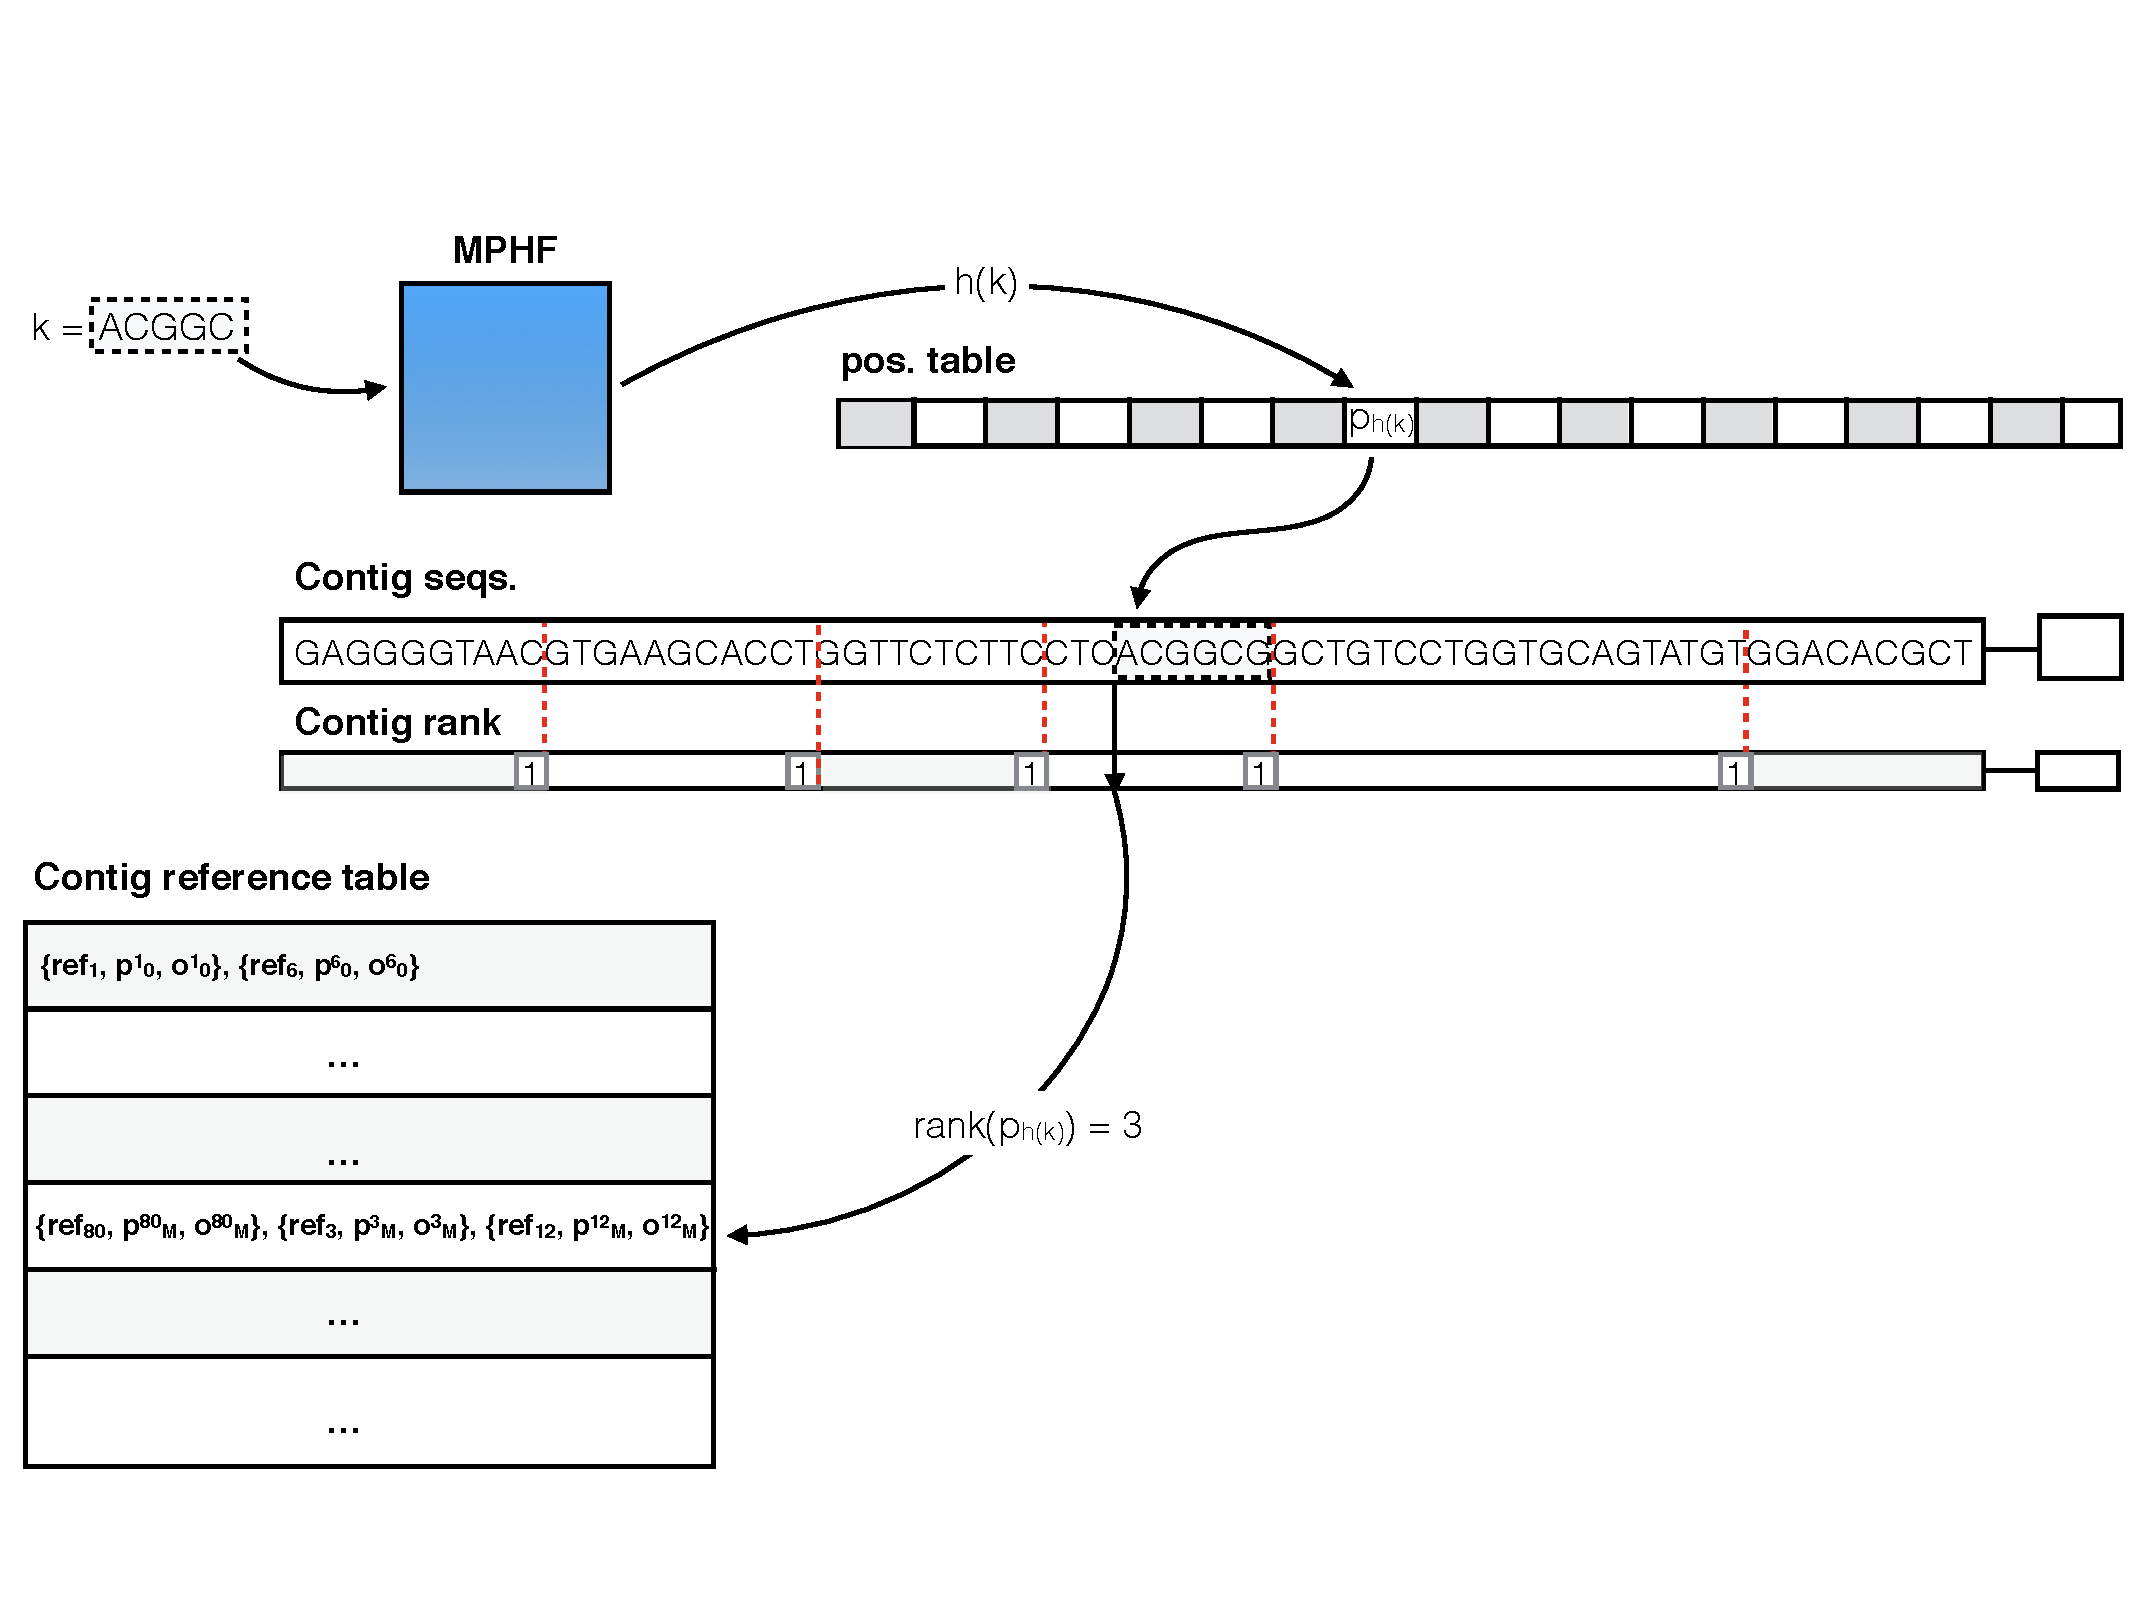
\includegraphics[width=\textwidth]{figs/index_fig}
\caption{An illustration of searching for a particular \kmer in the \emph{dense}
  \pufferfish index. The minimum perfect hash yields the index, $P_{h(x)}$ in the
  \emph{pos} vector where the \kmer appears in the contig array. The \kmer is
  validated against the sequence recorded at this position (and, in this case,
  it matches). A rank operation on $p_{h(x)}$ is performed in the boundary
  vector, which yields the corresponding contig-level information in the contig
  table. If desired, the relative position of the \kmer within the contig can be
  retrieved with an extra select and rank operation.}
\label{fig:dense_index}
\end{figure}


\section{Methods}\label{sec:methods}

We introduce a new data structure, implemented in the software \pufferfish, for
indexing the \ccdbg (and colored variants of it). While we are conscious of
memory usage, we don't aim to build the smallest possible index. Rather, we care
about making the \ccdbg index practical for genomic and metagenomic data while
maintaining very fast query speeds over the index. Here, we introduce both a
\emph{dense} and \emph{sparse} variant of the \pufferfish index, where, as with the
FM-index~\cite{Ferragina2001Experimental}, the sparsity factor can be tuned to
trade off search speed for index size. The sparse index tuned to take maximum space,
is at the same level as dense index regarding space and \kmer query time.

\paragraph*{Pre-processing} We assume as input to \pufferfish, the \ccdbg on the reference
or set of references to be indexed. The \pufferfish software itself accepts as input
a graphical fragment assembly (GFA) format file that describes the \ccdbg.
Specifically, this file encodes the contigs (i.e., non-branching paths) of the
\ccdbg as ``segments'' and the mapping between these contigs and the original
reference sequences as ``paths''. Each path is spelled out with an ordered set of contig IDs and the orientation they are mapped by, so that each contig has an overlap of k-1 with its following contig in the path (either in forward or reverse-complement).
The GFA is an evolving standard that is meant
to be a common format used by tools dealing with graphical representations of
genomes or collections of genomes. We note that there are a number of software
tools for building the \ccdbg directly (i.e., without first building the
un-compacted \dbg). We adopt \twopaco~\cite{minkin2016twopaco}, which employs a
time and memory-efficient, parallel algorithm for directly constructing the
\ccdbg, which can then easily be converted into GFA format. We note that, due to
a technical detail in the way \twopaco constructs the \ccdbg and the GFA file,
this output cannot be used directly, so \pufferfish includes a GFA-to-GFA converter
that prepares the \twopaco-generated GFA file for indexing by
\pufferfish\footnote{Specifically, the \twopaco \ccdbg has two main differences with
  the format that is expected by \pufferfish. First, it is not the case that \kmers
  and their reverse complements will appear only once in the \twopaco \ccdbg.
  Second, the GFA generated by \twopaco assumes that \emph{edges} of size at
  least $k+1$ will act as GFA segments, implying that they will overlap by $k$
  nucleotides. However, we require that segments be of at least size $k$ and
  overlap by exactly $k-1$ nucleotides.}.

\subsection*{The dense \pufferfish index}

Here we describe the basic (i.e., dense) \pufferfish index. The index consists of 6
components, each of which is described below:

\begin{enumerate}

\item The contig sequence array (\cseq) consists of the (2-bit encoded) sequence of all
  contigs of the \ccdbg packed together into a single array. Typically, the size
  of this structure is close to (or smaller than) the size of the 2-bit encoded
  reference sequence, since redundant sequences are represented only once in
  this structure. We note that the contig array contains the sequence of every
  valid \kmer, as well as that of potentially invalid \kmers (those which span
  contig boundaries in the packed array as the contig sequences in the array follow each other without any delimiters or gaps.).
  Therefore, using the next data structure we will set the boundaries of contigs in the array in a way that makes retrieving the borders, knowing position of a contig in the contig array and length of the contig fast in the query process. 
  We denote by $L_s$ the total length (in
  nucleotides) of the contig array.

\item The boundary vector (\bv) is a sparse bit-vector with a length of $L_s$
  bits. The bits of this vector are in one-to-one correspondence with the
  nucleotides of the contig array, and the boundary vector contains a one at
  each nucleotide corresponding to the end of a contig in the contig array, and
  a zero everywhere else. We can retrieve rank of each contig in \cseq using the
  \rank~operation on \bv. $\rank(\bv[i])$ returns number of 1s in \bv before the current index, $i$, or in other words the rank of the current contig. This can be used to get reference information for the current contig from \ctab, the data structure explained in item \ref{items:dense5}.

\item The minimum perfect hash function ($h\left(\right)$) maps every
  \emph{valid} \kmer in the contig array (i.e., all \kmers not spanning contig
  boundaries) to a unique number in $\left[0,N\right)$, where $N$ is the number
    of distinct valid \kmers in \cseq. We make use of the highly-scalable MPHF
    construction algorithm of~\cite{limasset2017fast}.

\item The position vector (\emph{pos}) stores, for each valid \kmer $x$, the
  position where this \kmer occurs in \cseq. Specifically, for \kmer $x$,
  \emph{pos}$\left[h\left(x\right)\right]$ contains the starting position of $x$ in \cseq 
  such that $\cseq\left[h\left(x\right),h\left(x\right) + k\right] = x$.

\item The conitg table \ctab stores, for each contig appearing in \cseq, the reference
  sequences (including reference ID, offset and orientation) where this contig appears in the
  reference. This is similar to a ``posting list'' in traditional inverted
  indices, where all occurrences of the item (in this case, an entire \ccdbg
  contig) are listed. The order of the contigs in the contig table is the same
  as their order in \cseq, allowing the information for a contig to be accessed
  via a simple rank operation on \bv.

\label{items:dense5}

\item \emph{Optionally}, an equivalence class table that records, for each
  contig, the set of reference sequences where this contig appears.
  Pre-computation and storage of these equivalence classes can speed up fast
  mapping approaches (e.g., pseudoalignment).

\end{enumerate}

These structures allow us to index every \kmer in the \ccdbg efficiently, and to
recall, on demand, all of the reference loci where this \kmer occurs. We note
here that the \kmers of the \ccdbg constitute only a subset of the \kmers in
\cseq. We refer to all \kmers in \cseq that do not span the boundary between two
contigs as \emph{valid} \kmers; these are in one-to-one correspondence with the
\kmers of the \ccdbg.

\subsubsection*{\kmer query in the dense \pufferfish index}
By using a MPHF $h$ to index the \emph{valid} \kmers, we avoid the typically
large memory burden associated with standard hashing approaches. Instead, the
identity of the hashed keys is encoded implicitly in \cseq. Given a \kmer $x$, we
can check for its existence and location in the following way. We first compute
$i = h(x)$, the index assigned to \kmer $x$ by $h$. If $i > N$, then we
immediately know that $x$ is not a valid \kmer. Otherwise, we retrieve the
position $p_{i}$ stored in $\texttt{pos}[i]$. Finally, we check if the encoded
string $\cseq[i:i+k]$ is identical to $x$. If so, we have found the
contig location of this \kmer, otherwise, $x$ is not a valid \kmer. 

Given $p_{i}$, we can retrieve the reference positions by computing $r_{p_i} =
\rank(\bv[p_{i}])$, which provides an index into \ctab that is
associated with the appropriate contig. This provides all of the reference
sequences, offsets and orientations where this contig appears. We compute the
offset of \kmer $x$ in the contig as $o_{i} = p_{i} - \select(r_{p_i})$,
in which \select returns the start position of the contig in \ctab.
This allows us to easily project this \kmer's position onto each reference
sequence where it appears. We note that querying a \kmer in the \pufferfish index is
an asymptotically constant-time operation, and that the reference loci for a
\kmer $x$ can be retrieve in $O(\texttt{occ}(x))$ time, where $\texttt{occ}(x)$
is the number of occurrences of $x$ in the reference.

\subsection*{The sparse \pufferfish index}

The \pufferfish index, as described above, is relatively memory-efficient. Yet, what
is typically the biggest component, the \texttt{pos} vector, can still grow rather
large. This is because it occupies $\lg(L_s)$ bits for each of the $N$ valid
\kmers in \cseq. However, at the cost of a slight increase in the practical
(though not asymptotic) complexity of lookup, the size of this structure can be
reduced considerably. To see how, we first make the following observation:

\begin{observation}
  In the \ccdbg (and hence, in \cseq), each valid \kmer occurs exactly once (\kmers occuring between contig boundaries are not considered).
\end{observation}

Hence, any valid \kmer in the \ccdbg is either a complex \kmer (i.e., it has an
in or out degree greater than 1), is a terminal \kmer (i.e., it appears at the
beginning or end of some input reference sequence), or it has a unique
predecessor and successor in the orientation defined by the contig.

We can exploit this observation in \pufferfish to allow \emph{sampling} of the \kmer
positions. That is, rather than storing the position of each \kmer in the contig
array, we store the position only for some subset of \kmers, where the rate of
sampling is defined by a user-defined parameter $s$. For those \kmers that are
not sampled, we store, instead, four pieces of information; the extension that
must be applied to move toward the closest \kmer at a sampled position, whether
or not the corresponding \kmer in \cseq is canonical, whether the extension
to reach the nearest sampled position should be applied by moving to the left or
the right, and a bit vector with the same size as \cseq
that is set to $1$ for any \kmer in \cseq that we've stored its position and $0$
for those that are not sampled.
This idea of sampling the positions for the \kmers is similar to the
idea of sampling the suffix array positions that is employed in the
FM-index~\cite{Ferragina2001Experimental}. This allows us to trade off query
time for index space, to allow the \pufferfish index to scale to large genomes or
collections of genomes. 


\subsubsection*{\kmer query in the sparse \pufferfish index}  \kmer query in the sparse \pufferfish index
is the same as that in the dense index, except for the first step ---
determining the position of the \kmer $x$ in \cseq. When we query the MPHF with
$x$ to obtain $i = h(x)$, there are three possible results. 
\begin{enumerate}
\item In the first case,
we could have that $i \geq N$, implying, just as in the dense case, that $x$ is
not a valid \kmer. 
\item Second, we could have that $\texttt{sampled}[i] = 1$,
implying that we have explicitly stored the position for the $i$-th \kmer, in
which case we can retrieve that position as $p_{i} = \texttt{pos}[\texttt{rank}(\texttt{sampled}[i])]$ and
proceed as before in the dense case to validate $x$ and retrieve its reference positions.
\item The third case is that $i < N$ and $\texttt{sampled}[i] = 0$. In this case, we do not know
the position where $x$ would occur in \cseq, and we must find the closest sampled position.
This is done with algorithm \ref{alg:nextSample}
\end{enumerate}

\begin{algorithm}
\caption{Find Next Sample}\label{alg:nextSample}
\begin{algorithmic}[1]
\Procedure{FindNextSample}{}
\State $\textit{e} \gets \textit{extension} \text{ size}$
\State $X \gets \textit{\kmer}$
\State $EV \gets \text{extension vector}$

\State $i \gets \textit{MPHF(\kmer)}$
\State $X_{rc} \gets \textit{reverseComplement}(X)$
%\BState \emph{loop}:
\While{\textbf{not} $isSampled[i]$} 

%\If {$isSampled[i]$}
%\State \textbf{goto} \emph{end}.
%\EndIf
\State $extIdx \gets i-rank(isSampled[i])$
\If {$isCanonical[i]$ \textbf{and} $isDirectionRight[i]$}
\State $X \gets X[e:] + EV[extIdx]$.
\EndIf
\If {\textbf{not} $isCanonical[i]$ \textbf{and} $isDirectionRight[i]$}
\State $X \gets X_{rc}[e:] + EV[extIdx]$.
\EndIf
\If {$isCanonical[i]$ \textbf{and} \textbf{not} $isDirectionRight[i]$}
\State $X \gets EV[extIdx] + X[:-e]$.
\EndIf
\If {\textbf{not} $isCanonical[i]$ \textbf{and} \textbf{not} $isDirectionRight[i]$}
\State $X \gets EV[extIdx] + X_{rc}[:-e]$.
\EndIf
\State $i \gets \textit{MPHF(\kmer)}$
\State $X_{rc} \gets \textit{reverseComplement}(X)$
\EndWhile
%\BState \emph{end}:
\Return $X$
\EndProcedure
\end{algorithmic}
\end{algorithm}


Intuitively, algorithm \ref{alg:nextSample} appends nucleotides stored in the
\texttt{extension} array to $x$ to generate a new \kmer, $x'$ which either has a
sampled position, or is closer to a sampled position than is $x$. The extension
process is repeated with $x'$, $x''$, etc. until a sampled position is reached.
At that point, one simply traverses back to the position in \cseq implied by the
sampled position and sequence of extension operations, for the original \kmer
$x$. The rest of the search proceeds as for the dense case. The whole process of
\kmer query in sparse index is illustrated in Fig \ref{fig:sparse_query} through an example.

\begin{figure}
  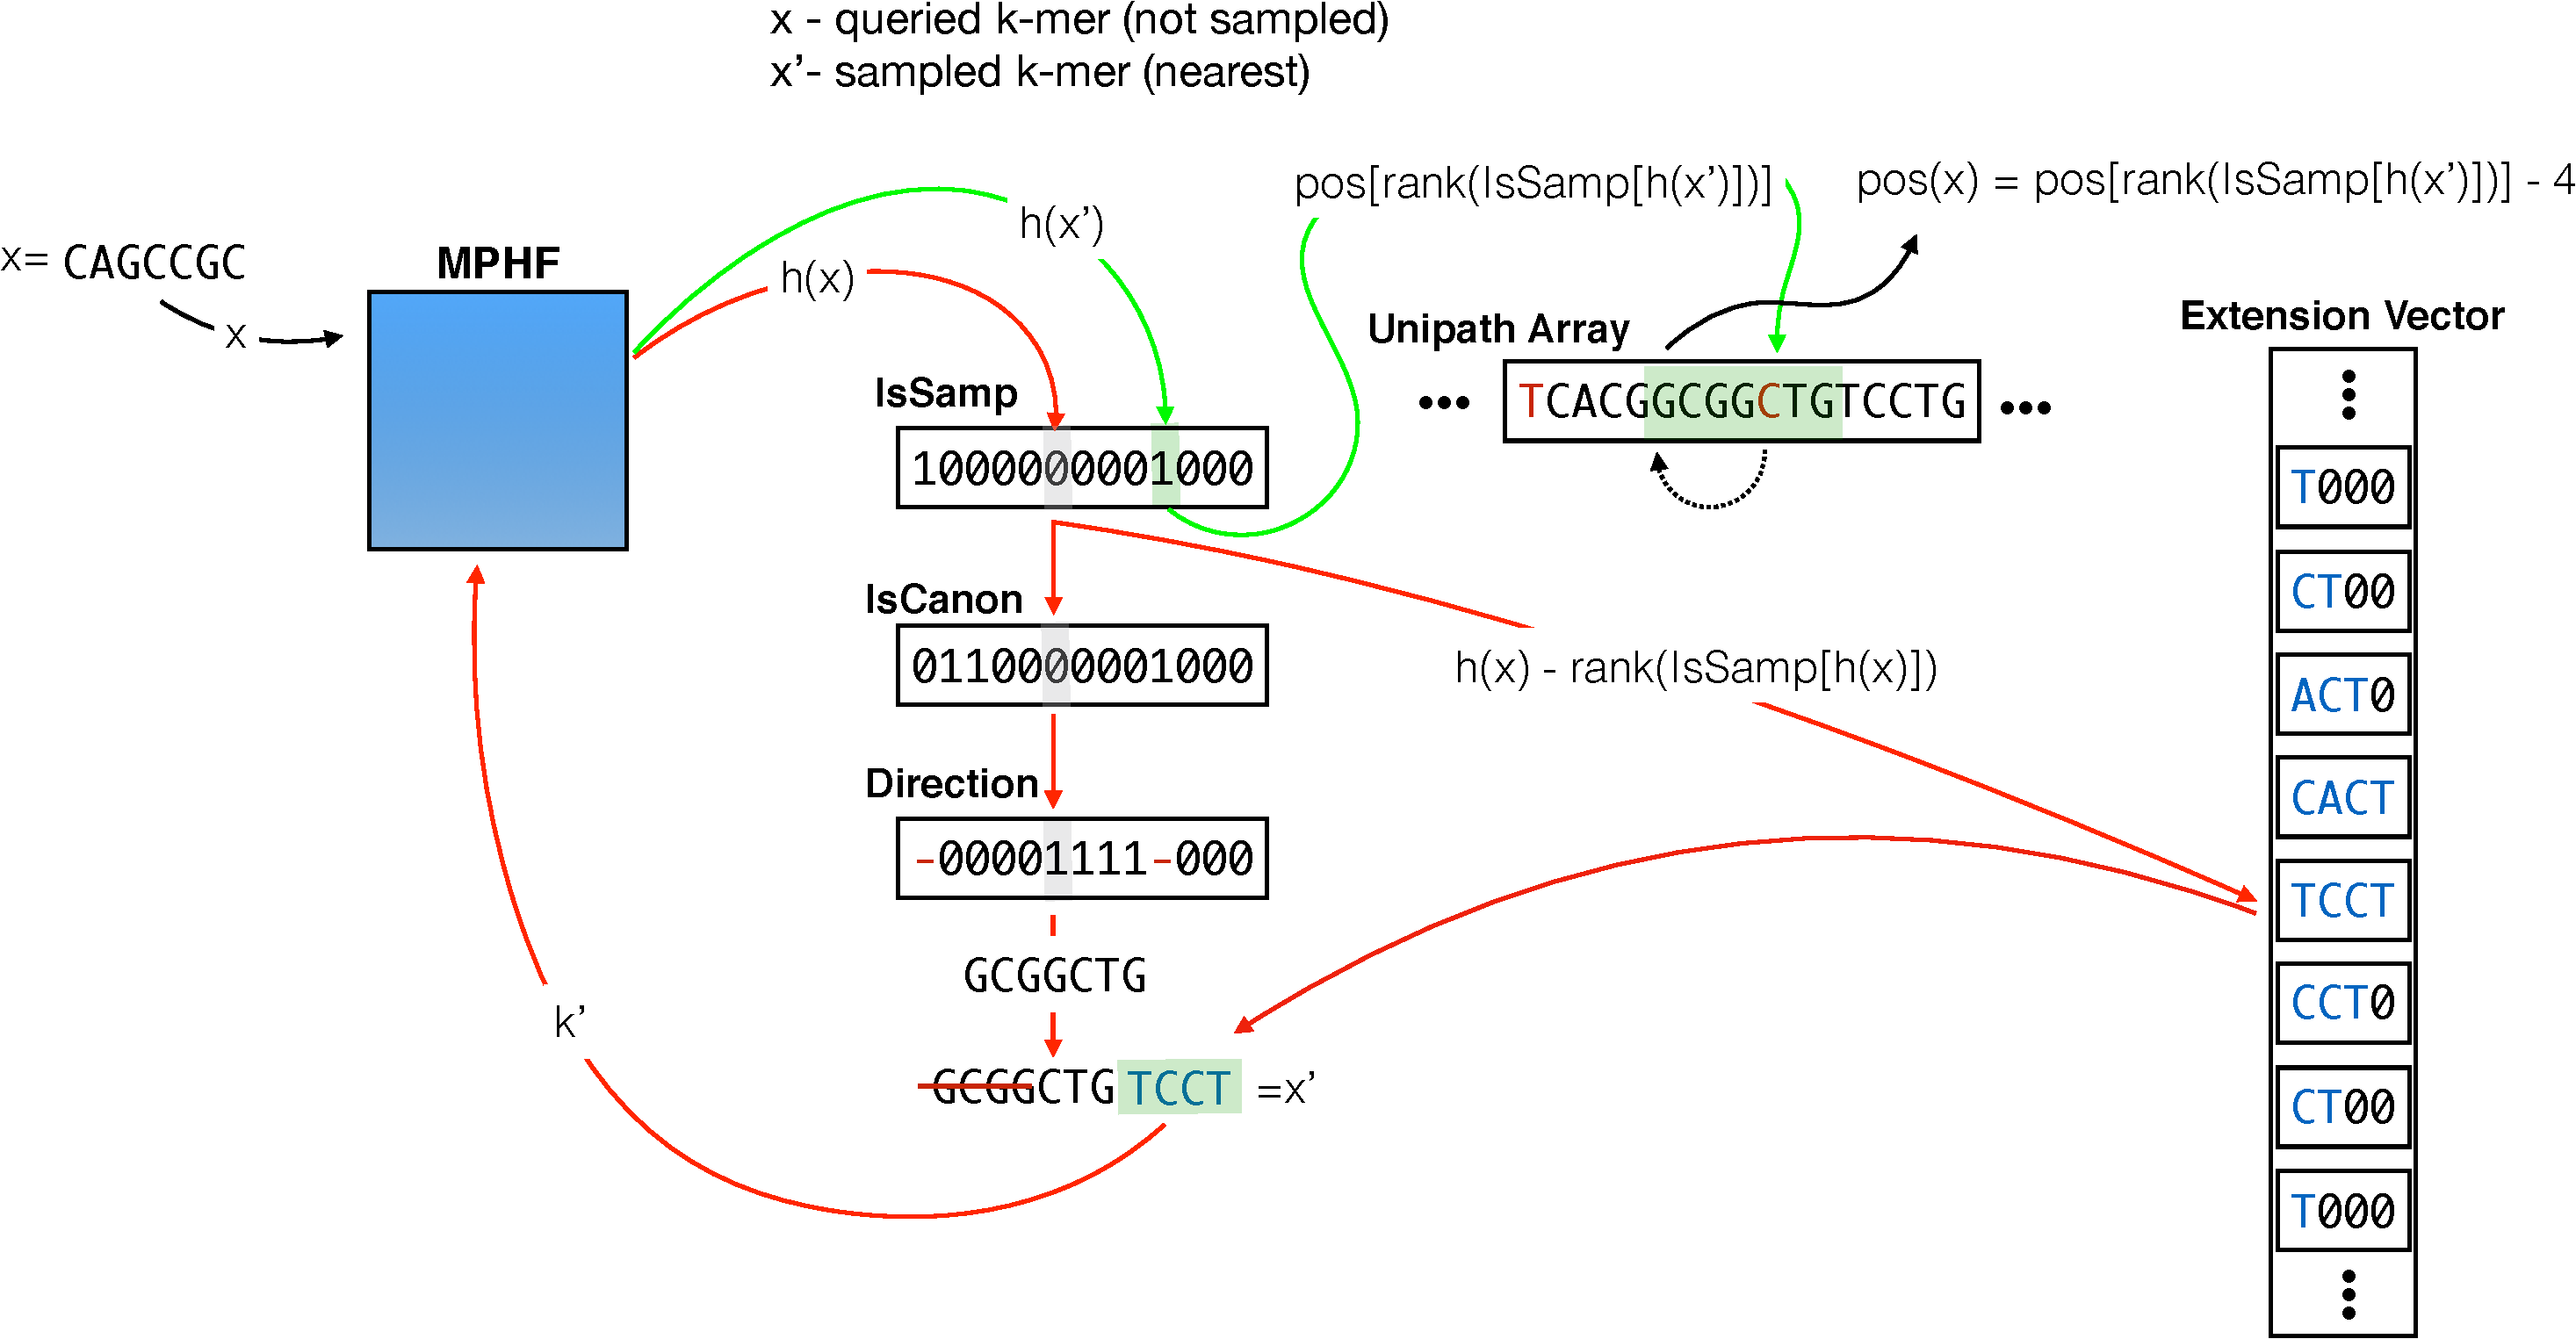
\includegraphics[width=\textwidth]{figs/query_sparse}
\caption{An illustration of searching for a particular \kmer in the \emph{sparse}
  \pufferfish index with sample factor ($s$) of 9 and extension size ($e$) of 4.
  All vectors \emph{isSampled}, \emph{isCanon}, and \emph{ExtRight} have the same
  size which is equal to length of the total number of valid \kmers.
  The minimum perfect hash yields the index, $h(x)$ for $x=CAGCCGC$ in the
  \emph{isSampled} vector where we'll find out that the \kmer is not sampled.
  \emph{isCanon} being $0$ at the same index as $h(x)$ shows that the \kmer
  is not canonical. Since we keep the extensions in canonical format we need to 
  canonicalize the \kmer to $x'=GCGGCTG$ first. Then based on the value of 
  $\text{\emph{ExtRight}}_{h(x)}$, we know that to get to the closest sampled \kmer
  we need to append the extension to the right of the current \kmer.
  The extension is extracted from \emph{QueryExt} vector. Considering the fact
  that we just keep the extensions for \kmers that are not sampled,
  to find the index of the current \kmer's extension we need to
  subtract the index of the \kmer by total number
  of \kmers that have been sampled up to this position which is equal to 
  total number of $1$s in \emph{isSampled} vector before $h(x)$ for which we use the
  \emph{rank} operation. Therefore, the extension index will be $h(x)-rank(isSampled[h(x)])$.
  We create the new \kmer $x'$ by cropping the first four bases off the current \kmer and
  appending the new extension to its right and repeat the same process for the new \kmer.
  This time, the \kmer is sampled and hence, we go directly to the index in the \emph{UnipathArray}
  that the \emph{sampledPos} vector points us to. To check if the original \kmer we searched for
  exists, we need to compare the \kmer starting from $4$ bases before the current position 
  with the canonic of original \kmer $x=CAGCCGC$ since we just appended one extension of size 4
  to the end of this \kmer. Generally speaking, we need to revert all the extension appendings 
  by walking over the \emph{UnipathArray} vector to the left and right with the same steps as
  extension size until we stop at the right position that we expect the \kmer at that position to be the
  same as the one we searched.}
\label{fig:sparse_query}
\end{figure}



By altering the stored extension size $e$ and the maximum sampling rate $s$, one
can limit the maximum number of extension steps (and hence the maximum number of
hash lookups) that must be performed in order to retrieve the potential index of
$x$ in \cseq. A denser sampling and longer extensions require fewer possible
extension steps, while a sparser sampling and shorter extensions require less space
for each non-sampled position. If $e \geq \frac{s}{2}$, one can guarantee that
at most a single extension step needs to be performed for any \kmer query, which
allows \kmer queries to remain, practically very fast while still considerably
reducing the index size for large reference sequences.

Even though the sparse index maintains a number of extra bit vectors not maintained
in the dense index, it is still usually considerably smaller.
Assume a case where the extension length $e$ is half of the sampling factor $s$.
Since we keep the extension required to get to 
the closest position in left or right direction, we would need to keep
$\frac{s}{2}$ bases for a kmer with each base represented in 2 bits, which corresponds to 
$\frac{s}{2}\times 2 = s$ bits per \kmer for the extension vector. Therefore, if we put all the new 
vectors of extension, canonical, direction, and isSampled together it'll be $s+1+1+1=s+3$ bits 
per each non-sampled \kmer compared to $\lg(L_s)$ bits that we had to keep in 
\emph{pos} vector. Therefore, as long as $[s+3< \lg(L_s)]$ we save space by sparse indexing.
In a typical data set such as human genome with $\lg(L_s) \sim= \lg(3B) \geq 30$ bits, by choosing
$s=9$ which means we'll sample each 9th \kmer, we will save $\sim18$ bits per each non-sampled \kmer.
%\todo{put actual numbers}

\section{Results}\label{sec:results}

We explored the memory and time requirements for building a text index using
\pufferfish and two other tools, \bwa and \kallisto. We also benchmark the speed of
\kmer lookup (the fundamental building block of \bwa's alignment and \kallisto's
pesudoalignment) under these different data structures. We performed these
benchmarks on a number of different reference sequences, selected to show how
the different indexes scale as the underlying reference size and complexity
increase. \bwa and \kallisto both have the complete package for
indexing a data set. For \pufferfish however, we first need to build the \ccdbg using the available
tools. We build the \ccdbg and dump it in GFA format using \twopaco. Then, as the output does
not satisfy our definition of a compacted dbg, we need to have another preparation 
step to convert the GFA file. We call this process\emph{pufferization}, and it converts the GFA file to the format accepted by pufferfish
(each \kmer should be appear only once through out all the unitigs and unitigs should have an overlap of $k-1$ bases).
Then we will build both dense and sparse index and benchmark the time and memory for all these steps of the pipeline individually.
Final comparison between the time and memory that pufferfish requires versus the other tools should be the aggregated time and
maximum memory of the whole pufferfish pipeline.
All experiments
were performed on an Intel(R) Xeon(R) CPU (E5-2699 v4 @2.20GHz with 44 cores and
56MB L3 cache) with 512GB RAM and a 4TB TOSHIBA MG03ACA4 ATA HDD running ubuntu
16.10, and were carried out using a single thread except for cdBg building step using TwoPaCo.

%\todo{explain datasets}

\begin{table}
\begin{center}
\begin{tabular} {| l || c c c| c c c|}
\hline
\multirow{2}{*}{Indexing Tools} & \multicolumn{3}{c|}{Memory (MB)} & \multicolumn{3}{c|}{Time (secs)} \\
\cline{2-7}
& \parbox[c]{2.5cm}{Human\vfill Transcriptome} & 
\parbox[c]{1.5cm}{Human\vfill Genome} & 
\parbox[c]{1.5cm}{Bacterial \vfill Genome} & 
\parbox[c]{2.5cm}{Human \vfill Transcriptome} & 
\parbox[c]{1.5cm}{Human \vfill Genome} & 
\parbox[c]{1.5cm}{Bacterial \vfill Genome} \\
\hline
 
\bwa & 292 & 4,443 & 32,213 & 2:56 & 0:58:27 & 13:11:45\\
\hline
\kallisto & 3,552 & 150,657 & NA & 3:05 & 3:27:42 & >2 days\\
\hline
\twopaco & 1,466 & 18,004 & NA & 2:47 & 0:56:12 & >2 days \\
pufferize & 584 & 27,438 & 49,510 & 0:10 & 0:21:53 & 54:11\\
pufferfish dense & 438 &  20,000 & 30,224 & 1:16 & 0:51:20 & 1:27:08 \\
pufferfish sparse & 331 & 17,745 & 29,811 & 1:44 & 1:10:48 & 2:02:34\\
\hline
\end{tabular}
\caption{
  Construction time and memory for \pufferfish, \kallisto, and \bwa for different
  datasets. 
}
\vspace{-2.5em}
\label{tab:construction}
\end{center}
\end{table}

\begin{table}
\begin{center}
\begin{tabular} {| l || c c c| c c c|}
\hline
\multirow{2}{*}{Indexing Tools} & \multicolumn{3}{c|}{Memory (MB)} & \multicolumn{3}{c|}{Time (secs)} \\
\cline{2-7}
& \parbox[c]{2.5cm}{Human\vfill Transcriptome} & 
\parbox[c]{1.5cm}{Human\vfill Genome} & 
\parbox[c]{1.5cm}{Bacterial \vfill Genome} & 
\parbox[c]{2.5cm}{Human \vfill Transcriptome} & 
\parbox[c]{1.5cm}{Human \vfill Genome} & 
\parbox[c]{1.5cm}{Bacterial \vfill Genome} \\
\hline
 
         
  
\bwa & 308 & 4,440 & 33,333 & 1:09:14 & 1:11:29 & 6:41\\
\hline
\kallisto & 3,337 & 110,646 & 120,748 & 6:17 & 24:29 & 20:06\\
\hline
pufferfish dense & 500 & 17,661 & 28,596 & 6:05 & 16:14 & 3:34 \\
pufferfish sparse & 315 & 12,510 & 20,470 & 17:41 & 26:38 & 4:26\\
\hline
\end{tabular}
\caption{
  \kmer lookup time and memory for \pufferfish, \kallisto, and \bwa for different
  datasets. 
}
\vspace{-2.5em}
\label{tab:query}
\end{center}
\end{table}

As expected we see in table \ref{tab:construction} that \pufferfish takes longer to build the index compared to a linear indexing based
tool such as \bwa and stands almost in the same level as \kallisto which is another graph-based indexing tool. 
However, the amount of memory it needs is considerably smaller than \kallisto, so that for a large reference
such as the human genome, it consumes $\sim6$ times less memory. Comparing the \kmer lookup time in table \ref{tab:query}, 
we can see how using a graph-based indexing system can outperform \bwa regarding time and still because of the succinct
data structures used in the index building and the compression algorithms used in that would need almost the same memory as \bwa
which is much less than what \kallisto needs to load all the indexing data structure.
The disk space and memory \pufferfish needs are very similar, unlike \kallisto, where the hash table consumes
much more RAM than what serialized version requires on disk.

\begin{table}
\begin{center}
\begin{tabular} {| l || c c c |}
\hline
\parbox[c]{2cm}{Indexing \vfill Tools} & 
\parbox[c]{2.5cm}{Human\vfill Transcriptome} & 
\parbox[c]{1.5cm}{Human\vfill Genome} & 
\parbox[c]{1.5cm}{Bacterial \vfill Genome}  \\
\hline   
       
\bwa & 347M & 5.12G & 37.8G \\
\hline
\kallisto & 1.7G & 58G & 87G \\
\hline
pufferfish dense & 387M & 16G & 26G \\
pufferfish sparse & 271M & 11G & 18G \\
\hline
\end{tabular}
\caption{
  Disk space each of \pufferfish, \kallisto, and \bwa will take for different
  datasets. 
}
\vspace{-2.5em}
\label{tab:disk-space}
\end{center}
\end{table}
%kallisto construction on GRCh38 (primary)
%%
%rob@newton:~ /usr/bin/time ~/kallistokmerlookup/build/src/kallisto index -k 31 -i GRCh38.primary\_assembly.genome.fixed.kalidx GRCh38.primary\_assembly.genome.fixed.fa
%
%[build] loading fasta file GRCh38.primary\_assembly.genome.fixed.fa
%[build] k-mer length: 31
%[build] counting k-mers ... done.
%[build] building target de Bruijn graph ...  done
%[build] creating equivalence classes ...  done
%[build] target de Bruijn graph has 38967126 contigs and contains 2652229049 k-mers
%
%7911.72user 1873.99system 2:45:24elapsed 98\%CPU (0avgtext+0avgdata 154270332maxresident)k
%0inputs+119758728outputs (0major+3389704442minor)pagefaults 0swaps
%%

We note that on large sequences (e.g., the human genome)
kallisto seems to require an inordinate amount of time (i.e., days) to load the index into memory. This appears to
occur during the final phase of index loading. However, we were able to resolve this issue and hence
provide \kmer query times for these samples (otherwise just amortizing the index loading time over each \kmer would result
in lookup times tens of thousands of times slower than the other tools).

\section{Conclusion and Future Work}
In this chapter we proposed a new efficient data structure for indexing compacted de Bruijn graphs and also its implementation in a tool called \pufferfish. We showed how \pufferfish can achieve a balance between time and space resources. By building upon a MPHF~\cite{limasset2017fast}, we provide practically fast \kmer lookup, and by carefully organizing our data structure and making use of succinct representations where applicable, we greatly reduce the space compared to traditional hashing-based implementations. The main components of the data structures are a minimum perfect hash function (MPHF) built on \kmers, the concatenated unitig array from which the \kmers are sampled, a bit vector that marks the boundary of unitigs in the concatenated array, a vector containing the offset position for the \kmers, and a unitig table enumerating the occurrences of each unitig in the reference sequence.

Moreover, we presented two variants of the \pufferfish data structure; namely, a dense and a sparse variant. The first is optimized for fast queries and the second provides the user with the ability to trade off space for speed in a fine-grained manner. In the sparse index, we only keep offset positions for a subset of \kmers. To query an unsampled \kmer, the sparse representation is aided with a few auxiliary data structures of much smaller size. Since the largest component of the index is the position vector, adopting this sparse representation significantly reduces the required memory and disk space. Our analyses suggest that pufferfish (dense) achieves similar speed to existing hash-based approaches, while greatly reducing the memory and disk space required for indexing. We consider indexing and query on both small (human transcriptome) and large (~8000 bacterial genomes) reference datasets. Pufferfish strikes a desirable balance between speed and space usage, and allows for fast search on large reference sequences, using moderate memory resources. 

Having built an index for a reference genome or transcriptome using \pufferfish, the immediate future work would be implementing the applications of such an index. These applications fall into the categories that need mapping or alignment as their initial step. Therefore, we would like to adopt an existing aligner or mapper such as RapMap~\cite{srivastava2016rapmap} or Selective Alignement~\cite{sarkar2017towards} and modify it to use \pufferfish as its indexing methodology. Later we can use the result of this aligner for RNA-sequence quantification, metagenomic abundance estimation, or population-level read tasks. We expect the memory efficiency of \pufferfish indexing will be beneficial in working with larger collections of genomic and transcriptomic data sets. Moreover, by indexing the genome and transcriptome together using \pufferfish, we can discover novel exon splicing. 
%Genome comparison and structural variant detection in a group of genomes can also be one of the immediate results of the \pufferfish as construction and query time are both reasonably fast and also memory-efficient.


%%
%% Author: fatemeh
%% 2019-11-25
%%

\chapter{Going Beyond Limitation in Sequence Analyses}

In this chapter, ...




\section{Timeline}

\begin{center}
    \begin{tabular}{|l|c|}
        \hline
        \emph{de novo} clustering of scaffolds in SALSA & 2 months \\
        16s rRNA sequence clustering & 3-4 months\\
        Modifying and testing Bambus-3 contig layout algorithm & 1-2 months \\
        Phased scaffolding with Hi-C like data & 4-5 months \\
        Thesis writing & 4-5 months\\
        \hline
        \textbf{TOTAL} & 11-13 months \\
        \hline
    \end{tabular}
\end{center}

Paper deadline goals:

\begin{itemize}
    \item Genome Research, July  2017: Metagenome scaffolding and variant detection with Bambus3
    \item Bioinformatics, June  2017: DNAClust 2: Clustering 16s rRNA sequences with provable guarantees
    \item Nature Biotechnology, October 2017: Chromosome level phased assembly of hummingbird genome with different sequencing technologies
\end{itemize}



\chapter{Conclusion}

When working at the scale of whole genomes,
the problem of extending indexing strategies to graphs becomes very important.
In addition to that, indexing more than one sample in the same data structure
adds to the complexity of the problem.
In this document, we presented three data structures
for indexing a collection of genomes, transcriptomes, or sample reads
in the form of a colored de Bruijn graph or a compacted colored de Bruijn graph.
As future direction, we are interested in exploring the application
of one of these data structures, Pufferfish, in metagenomic analyses.

Another area of interest towards improving space efficiency of \cdbgs
can be exploring other ways to use fewer colors to represent all samples instead of compressing the color matrix. One idea, we have been discussing with Travis Gagie and Christina Bousher for potential collaborations, is to reuse the previously assigned colors in disjoint subgraphs and non-adjacent edges. In other words, we cannot reuse the same color for a different sample for \kmers that are adjacent, but we can have colors that are globally reused. In this case, we need to have a proper mapping from a color to its corresponding samples in different disjoint areas of the graph. As a de Bruijn graph is a special type of directed graphs with each node having at most $4$ incoming and $4$ outgoing edges, the chromatic number of such a graph is at most $9$ (maximum degree + 1~\footnote{Brooks' theorem})~\cite{cranston2015brooks}. Therefore, if we can design an efficient color-to-sample mapping, we can reduce the colors in the graph and skip assigning one bit to each color. In this case, we are approaching the problem from a different direction, rather than compressing the color matrix that we explained in~\ref{chap:rainbowfish}.

In the third chapter, we talked about a new indexing tool, \pufferfish. The main advantage of a data structure like \pufferfish compared to a linear index is the ability to efficiently map reads to a population of genomes or individual genomes with annotated variants. Current tools that are used for alignment and mapping are either suitable for genome or transcriptome, but not both. \pufferfish fills the gap by allowing fast and accurate mapping to a collection of genomes and transcriptomes at the same time. This ability paves the way for accomplishing applications such as novel exon discovery or RNA-seq quality control. 
Because of the distinction between methods that map to the transcriptome and those that map to the genome, we lose information that can be derived by putting both of these mappings together. One immediate outcome of having short reads mapped to both genome and transcriptome is in RNA-seq quality control. If we just look at the transcriptome mapping outcome, we could simply throw all the non-mapped reads out, ignoring the fact that not being mapped at all is a different observation than being mapped to an intron. A large fraction of reads mapping to introns is an evidence that the RNA-seq experiment failed to provide the required quality. Having reads that map to both the genome and transcriptome, we can account for such an experiment's failure. Another application of dual mapping, that is of biological importance, is looking for any intron retention in an RNA-seq experiment. High probability of retaining introns in reads from RNA-seq experiments is known to be associated with certain disease phenotypes~\cite{faustino2003pre,tazi2009alternative}. By mapping the reads to just transcriptomes, we can never be aware of intron retention statistics.

Another problem that can be answered using \pufferfish is finding structureal variations in a metagenomic data set or across different samples of the same individual~\cite{korbel2007paired,tuzun2005fine}.
One particular way to approach this problem is through genome alignment~\cite{korbel2007paired}.
Having a genome indexed using \pufferfish,
we can map another genome to it instead of a set of short reads.
In a similar way, we can index multiple genomes at the same time into one data structure
combining the concepts of indexing a colored de Bruijn graph and a compacted de Bruijn graph.
There are a lot of small scale variations happening across two genomes
that can be the result of an error in the read sequencing process or that may not be informative enough.
However, many biologically interesting variations across genomes happen at scales longer
than the length of the read.
Building \pufferfish along a collection of genomes will allow us to search for such variations.
One specific type of variation can be inversions between genomes where an interval of one genome is the same as the other, but inverted~\cite{feuk2010inversion,turner2006assaying}.
%, so that we have a one-to-one correspondence between \kmers of two separate genomes and at some location the positions start decreasing in one genome as we increase position in the other. 
The inversions can be identified by a data structure like \pufferfish that keeps position of a \kmer in all the references.


%\bibliographystyle{plainnat}
%\bibliography{introduction,merged,pufferfish,mantis,bibliography}
\bibliography{all}
%\input{bibliography}

    \newpage
    \input{ReadingList}


\end{document}